% =============================================================================
% Does Muon improve regulatory DNA learning?
% NeurIPS 2026 format
% =============================================================================

\documentclass{article}

% Use numerical citations instead of author-year
\PassOptionsToPackage{numbers, compress}{natbib}
\usepackage[main]{neurips_2026}

\usepackage[utf8]{inputenc}
\usepackage[T1]{fontenc}
\usepackage{hyperref}
\usepackage{url}
\usepackage{booktabs}
\usepackage{amsfonts}
\usepackage{amsmath,amssymb,amsthm}
\usepackage{nicefrac}
\usepackage{microtype}
\usepackage{xcolor}
\usepackage{graphicx}
\usepackage{subcaption}
\usepackage{float}
\usepackage{tikz}
\usetikzlibrary{arrows.meta, positioning}

\DeclareMathOperator*{\argmax}{arg\,max}

\renewcommand{\topfraction}{0.9}
\renewcommand{\bottomfraction}{0.9}
\renewcommand{\textfraction}{0.1}
\renewcommand{\floatpagefraction}{0.8}
\setcounter{topnumber}{3}
\setcounter{bottomnumber}{3}
\setcounter{totalnumber}{6}

\makeatletter
\newcommand{\supplementarylinknote}{%
  \if@anonymous\relax\else
    \noindent\emph{Supplementary material, including an interactive visualization, is available at \url{https://origin.bio/blogs/muon}.}%
  \fi
}
\makeatother

\title{Does Muon Improve Regulatory DNA Learning?}

\author{%
  Viraj Doshi \\
  Origin Bio \\
  \texttt{viraj@origin.bio} \\
}

\begin{document}

\maketitle

\begin{abstract}
Regulatory DNA models have the potential to improve design of gene therapies, but their use is succeeded by expensive biological testing. That makes training compute an upstream cost in the experimental pipeline, not just a modeling expense. We study whether optimizer choice can make this stage more compute-efficient by training the same ENCODE cCRE model with SGD, Adam, and Muon under different norm-control schemes. In a controlled sweep, the best Muon run reaches a fixed target test perplexity with approximately 31.6\% fewer FLOPs than the best Adam configuration. This suggests that regulatory DNA modeling still has substantial room for gains from new optimization and norm-control schemes.
\end{abstract}

% ============================================================
\section{Introduction}
\label{sec:intro}
% ============================================================

AI models trained on regulatory DNA now help prioritize variants, cis-regulatory elements, and gene-therapy design hypotheses before expensive biological follow-up. Systems such as AlphaGenome~\citep{alphagenome}, Enformer~\citep{enformer}, and Borzoi~\citep{borzoi} train on regulatory DNA and help decide which elements or perturbations to test, while downstream validation can require DNA synthesis, cloning, cell culture, and sequencing. Training compute is therefore upstream of costly experimental decisions: making this stage more efficient can shift resources from compute toward biological testing.

This is where optimizer choice becomes a very clear lever. We ask whether the same regulatory DNA model can reach a useful quality level with fewer training FLOPs. We test this by training on ENCODE candidate cis-regulatory elements while varying only the optimizer and the norm-control scheme. Because regulatory DNA differs from NLP, optimizer gains should be verified in-domain rather than assumed to transfer. We therefore include SGD baselines and compare Adam and Muon, each paired with either independent weight decay or Hyperball, across five learning rates and three model widths. The best Muon run reaches the best Adam target quality with approximately 31.6\% fewer training FLOPs, and the sweep suggests that there is still substantial room to explore optimization schemes tailored to regulatory DNA.


% ============================================================
\section{Related Work}
\label{sec:related-work}
% ============================================================

We are aware of two recent works that train or fine-tune DNA models with both Adam(W) and Muon, both of which have narrower experimental configurations, and neither of which reports a controlled FLOP-efficiency comparison, which is our central question to this investigation (as opposed to their convergence losses).

\paragraph{Pre-training genomic language models with variants~\citep{ukbiobert}.} Liu \emph{et al.} compare AdamW and Muon in a fine-tuning ablation for UKBioFormer and report no significant improvement from changing optimizers. However, the comparison is single-configuration: one downstream task, one metric, and one learning rate per optimizer, with no FLOP-efficiency analysis and no separation between optimizer choice and norm-control choice.

\paragraph{Foundation models for perturbation response~\citep{fmpert}.} Cole \emph{et al.} also report no significant difference between Adam and Muon, but again the comparison is narrow: only the learning rate is tuned, no FLOP-efficiency analysis is reported, and optimizer behavior is not separated from norm-control choices.

\paragraph{What this paper adds.} Both prior works draw the same null conclusion from single-point comparisons. We replace that design with a controlled $2\times 2$ sweep over \{Adam, Muon\} $\times$ \{independent weight decay, Hyperball\} across five learning rates and three model widths, and we measure FLOP-to-target rather than converged loss alone. Under this comparison, the best Muon run reaches the best Adam target quality with approximately $31.6\%$ fewer training FLOPs (Section~\ref{sec:results}, Appendix~\ref{app:flops}). The main methodological point is that optimizer conclusions change once norm control and compute efficiency are evaluated explicitly.


% ============================================================
\section{Distribution Differences}
\label{sec:distribution}
% ============================================================

\citet{wilson} showed that optimizer rankings change across domains: adaptive methods underperform SGD on some vision tasks despite converging faster, yet dominate SGD in language modeling. This is consistent with the No Free Lunch view~\citep{nfl} that optimizer performance depends on problem structure.
Regulatory DNA and natural language present very different sequence-learning problems. In language, much of the modeling burden comes from representing and composing meaning across a large semantic vocabulary. Regulatory DNA instead uses a compact four-letter alphabet whose predictive structure comes from how nucleotides are arranged into biochemical sequence patterns. Regulatory signal is carried by motif identity, motif strength, spacing, orientation, local composition, and combinations of nearby motifs, rather than by the standalone identity of a token. This makes regulatory DNA a distinct distributional setting for optimization: an optimizer that performs well on natural-language corpora is not guaranteed to behave the same way when the training signal comes from regulatory sequence grammar. Sequence-to-function models ultimately supervise on biological readouts such as expression, chromatin accessibility, or variant effects, but those predictions still depend on internal representations of this underlying regulatory sequence context. A nucleotide cross-entropy objective probes that sequence-distribution component directly: it tests how efficiently an optimizer learns the statistical structure of regulatory DNA before any task-specific functional head or supervised biological readout is added. Cross-entropy on regulatory DNA is therefore a relevant in-domain objective for studying optimization. This relationship between pretraining loss and biological utility is supported by recent foundation models. For instance, the Evo~2 model~\citep{evo2} demonstrated that scaling model parameters lowers validation loss, which in turn translates to broad improvements in zero-shot downstream performance across various genomic and molecular tasks. This confirms that perplexity serves as a strong proxy for downstream biological task performance in the genomic domain (Figure~\ref{fig:perplexity-downstream}).

\begin{figure}[htbp]
    \centering
    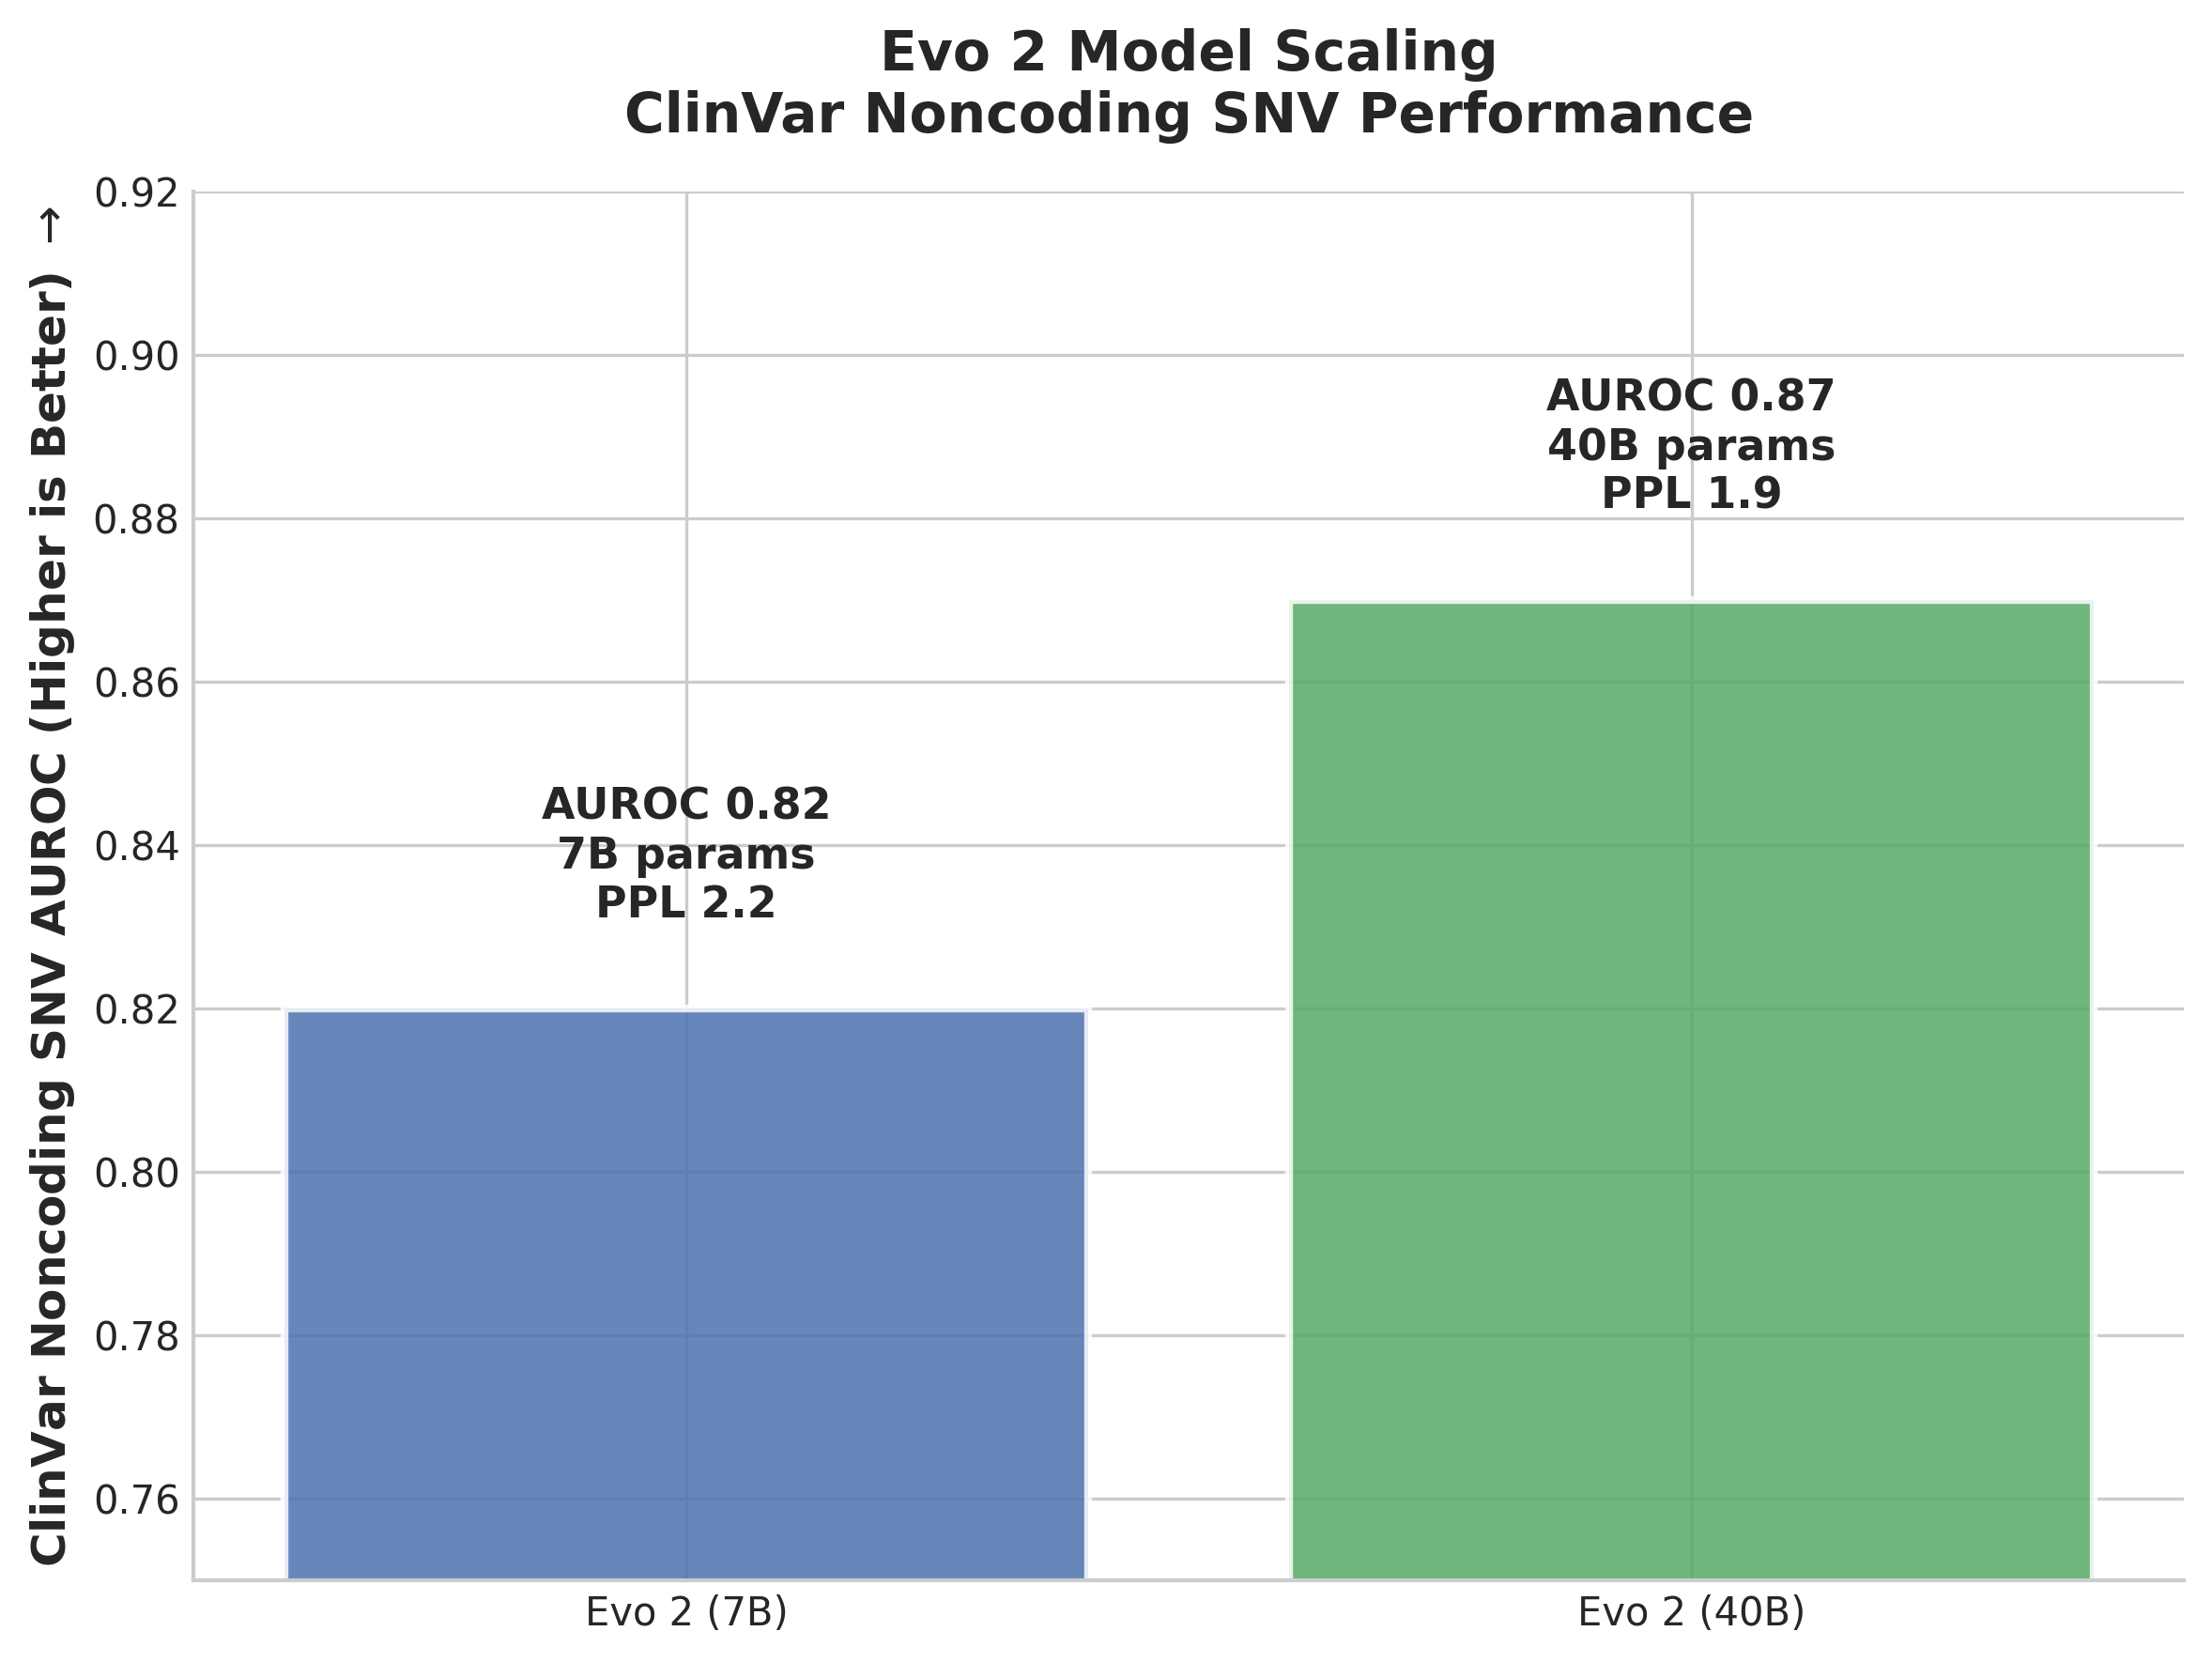
\includegraphics[width=0.85\linewidth]{images/Evo 2/evo_perplexity_vs_performance.png}
    \caption{Bar chart demonstrating the scaling laws of genomic foundation models: as validatlexity decreases from better scaling (e.g., from Evo 1 to Evo 2 7B and 40B), models yield proportionally higher performance on zero-shot downstream biological tasks (like ClinVar noncoding SNV AUROC), aligning with observations from Evo 2~\citep{2}.}
    \label{fig:perplexity-downstream}
\end{figure}

A high-level example of this distributional difference is the marginal token distribution. Nearly all modern optimizer benchmarks are run on natural language data, where token frequencies follow Zipf's law, with the $k$-th most common token appearing with frequency $f(k) \propto 1/k^\alpha$, typically with $\alpha \approx 1$. This produces a highly skewed vocabulary: a small number of tokens appear extremely often, while a long tail of rare tokens appears infrequently. In a large language-model vocabulary, the most common token can be orders of magnitude more frequent than a rare token. Regulatory DNA looks very different. It has only four nucleotide tokens, and in our training data the marginal frequencies across cell lines are close to uniform (Figure~\ref{fig:nucleotide-dist}). The entropy of the DNA token distribution is therefore close to its maximum, unlike language where Zipf concentration creates strong token imbalance.

This matters for optimization because token frequencies directly shape gradient statistics. If a mini-batch contains tokens with marginal probabilities $p_k$, then the expected contribution of token $k$ scales with $p_k$, and Adam's second-moment accumulator for token-associated parameters scales roughly as $v_k\propto p_k$ (Appendix~\ref{app:gradient-stats}). Under a Zipfian language distribution with $K\approx100{,}000$, the ratio between the largest and smallest token frequencies can be on the order of $10^5$, so Adam's $1/\sqrt{v_k}$ normalization can apply very different effective step sizes to common-token and rare-token directions. With DNA, $K=4$ and $p_k\approx1/4$, so this frequency-driven dynamic range is close to $1$. The adaptive denominator is correspondingly closer to a shared scalar across nucleotide-associated directions. Thus, optimizer rankings established on language corpora should therefore not be assumed to transfer cleanly to regulatory DNA.

% ============================================================
\section{Weight Regularization}
\label{sec:weight-reg}
% ============================================================

\subsection{Weight regularization controls optimizer step size}
\label{sec:weight-decay}

If the goal is to compare optimizers, then effect of different weight regularization methods must be considered. Without norm control, weight norms grow $\propto \sqrt t$ during training~\citep{hyperball}, changing parameter scale relative to step size and confounding the comparison~\citep{spectral-fl}. A sweep would then mix optimizer effects with uncontrolled norm drift.

Our first choice of regularization is weight decay, specifically independent weight decay, as opposed to learning-rate-coupled decay. It drives the norm toward an equilibrium value~\citep{wdeq,adamw,hyperball}, separating update \emph{direction} from overall parameter scale~\citep{wdeq}. We use independent rather than learning-rate-coupled decay because it is the variant explicitly designed for hyperparameter transfer~\citep{wdtransfer}, an important mechanism in real train pipelines so that tuning can be done swiftly and economically.

Independent weight decay is also not the only plausible answer. Although it drives the norm toward an equilibrium, the optimizer must still search over the shell created by those fluctuations. In an $n$-dimensional ball of radius $R$, the fraction of volume in an outer shell of thickness $\varepsilon$ is $1-(1-\varepsilon/R)^n$, which tends to $1$ as $n$ grows (Appendix~\ref{app:concentration}). Thus, even small norm fluctuations can leave a very large high-dimensional search region near the boundary. For RMSNorm-sandwiched layers, scalar rescaling of a weight matrix is also partly washed out by normalization: $\mathrm{RMSNorm}(\alpha Wx)\approx \mathrm{RMSNorm}(Wx)$ for $\alpha>0$ when numerical epsilons are negligible (Appendix~\ref{app:scale-inv}). That makes direction more important than scale and motivates a sharper alternative: fix the norm and optimize only direction.

\subsection{Hyperball as a norm control method}
\label{sec:hyperball}

Hyperball~\citep{hyperball} fixes the Frobenius norm of each weight matrix $W$ to the initial radius $R := \|W_0\|_F$ and sets the norm of the update $U$ to $\eta R$. This confines the weight matrix to a hypersphere of radius $R$. Suppose $\mathrm{Normalize}(A):=A/\|{A}\|_F$. Given an optimizer's proposed update step $\tilde u_t$, let the actual update be:
\[
U_t = -\eta R\,\mathrm{Normalize}(\tilde u_t),
\]
then let
\[
W_{t+1} = R\,\mathrm{Normalize}(W_t + U_t).
\]
This construction can be wrapped around any optimizer update, so it works with Adam and Muon alike. That enables the testing of an optimizer advantage survives a different norm-control rule.

\supplementarylinknote

\medskip

The useful takeaway is that Hyperball makes the learning rate an approximate relative-step-size dial. Hyperball fixes $\|W_t\|=R$, sets $\|U_t\|=\eta R$, and then retracts $W_t+U_t$ back to the radius-$R$ sphere. If $\gamma$ is the cosine similarity between $W_t$ and $U_t$, in the small-learning-rate regime, this simplifies to $\|\Delta W\|/\|W_t\|\approx \eta\sqrt{1-\gamma^2}$, which becomes $\approx\eta$ when the update is nearly orthogonal to the current weights (Appendix~\ref{app:derivation}).

\paragraph{Relative step size of weight decay.} Under weight decay, by contrast, the relative step size depends on the learning rate, decay coefficient, optimizer state, momentum coefficients, and training time~\citep{wdeq,hyperball,wdnorm}; Hyperball removes most of that coupling by fixing $\|W_t\|=R$ and $\|U_t\|=\eta R$. In our runs, MuonW's relative step size decreases as $\|W_t\|$ grows, while MuonH remains flatter at the level set by $\eta$ (Figures~\ref{fig:dynamics-stepsize} and~\ref{fig:dynamics-norms}).


% ============================================================
\section{Experimental Setup}
\label{sec:experimental-setup}
% ============================================================

To isolate the effect of the optimizer, we hold model architecture, dataset, training duration, and all non-optimizer hyperparameters constant across runs, varying the optimizer, the norm-control scheme, and the learning rate. We train a transformer architecture model on candidate cis-regulatory elements (cCREs) from the ENCODE v4 registry that are specific to one of seven cell lines (see Appendix~\ref{app:data}). We tokenize on a single nucleotide resolution, and train it on a masked language modeling (MLM) objective. Along with the standard MLM cross-entropy loss, we also give the model an auxillary task to predict DNase-seq tracks using a factorised poisson and multinomial loss, in order to sharpen its context understanding.

\begin{figure}[htbp]
  \centering
  \resizebox{\linewidth}{!}{%
  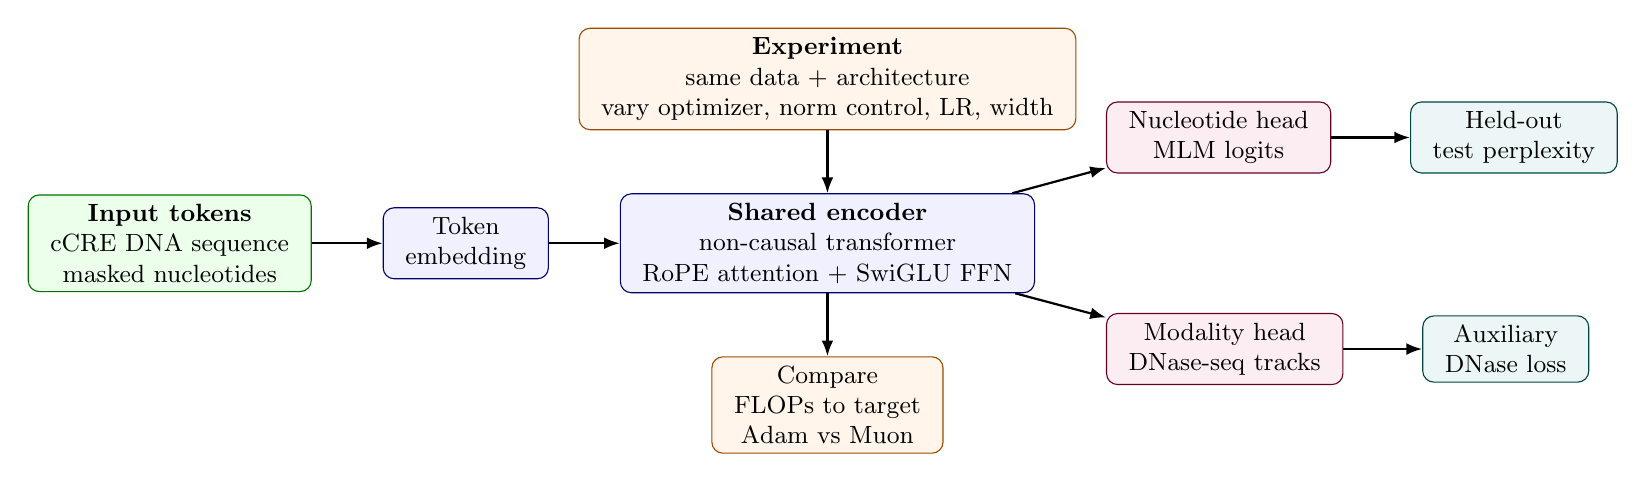
\begin{tikzpicture}[
    node distance=0.7cm and 0.9cm,
    box/.style={draw, rounded corners, align=center, minimum height=0.8cm, inner xsep=8pt, font=\small},
    dna/.style={box, fill=green!8, draw=green!45!black},
    model/.style={box, fill=blue!6, draw=blue!45!black},
    head/.style={box, fill=purple!7, draw=purple!55!black},
    opt/.style={box, fill=orange!8, draw=orange!60!black},
    data/.style={box, fill=teal!7, draw=teal!55!black},
    arrow/.style={-{Latex[length=2mm]}, thick}
  ]
    \node[dna] (input) {\textbf{Input tokens}\\cCRE DNA sequence\\masked nucleotides};
    \node[model, right=of input] (embed) {Token\\embedding};
    \node[model, right=of embed, minimum width=3.0cm] (encoder) {\textbf{Shared encoder}\\non-causal transformer\\RoPE attention + SwiGLU FFN};
    \node[head, above right=0.25cm and 0.9cm of encoder] (mlm) {Nucleotide head\\MLM logits};
    \node[head, below right=0.25cm and 0.9cm of encoder] (modality) {Modality head\\DNase-seq tracks};
    \node[data, right=1.0cm of mlm] (perplexity) {Held-out\\test perplexity};
    \node[data, right=1.0cm of modality] (dnase) {Auxiliary\\DNase loss};
    \node[opt, above=0.8cm of encoder] (experiment) {\textbf{Experiment}\\same data + architecture\\vary optimizer, norm control, LR, width};
    \node[opt, below=0.8cm of encoder] (compare) {Compare\\FLOPs to target\\Adam vs Muon};
    \draw[arrow] (input) -- (embed);
    \draw[arrow] (embed) -- (encoder);
    \draw[arrow] (encoder) -- (mlm);
    \draw[arrow] (encoder) -- (modality);
    \draw[arrow] (mlm) -- (perplexity);
    \draw[arrow] (modality) -- (dnase);
    \draw[arrow] (experiment) -- (encoder);
    \draw[arrow] (encoder) -- (compare);
  \end{tikzpicture}%
  }
  \caption{Experimental setup.}
  \label{fig:experimental-setup}
\end{figure}

Every run uses the same input pipeline, shared encoder, and two output heads. The nucleotide head supplies the MLM objective and held-out perplexity metric, while the modality head supplies the auxiliary DNase-seq prediction objective. The experiment changes only optimizer family, norm-control scheme, learning rate, and model width, then compares Adam and Muon by FLOPs required to reach a fixed test-perplexity target.

% ============================================================
\section{Results}
\label{sec:results}
% ============================================================

\subsection{Muon reaches Adam's lowest test perplexity with 31.6\% fewer flops}

Aggregating optimizer variants by family gives the clearest high-level view. Figure~\ref{fig:family-progressions} compares the best Adam and Muon family curves at the largest scale against both FLOPs and wall-clock time. In both views, Muon reaches lower perplexity sooner than Adam.

\begin{figure}[htbp]
  \centering
  \begin{subfigure}[t]{0.48\linewidth}
    \centering
    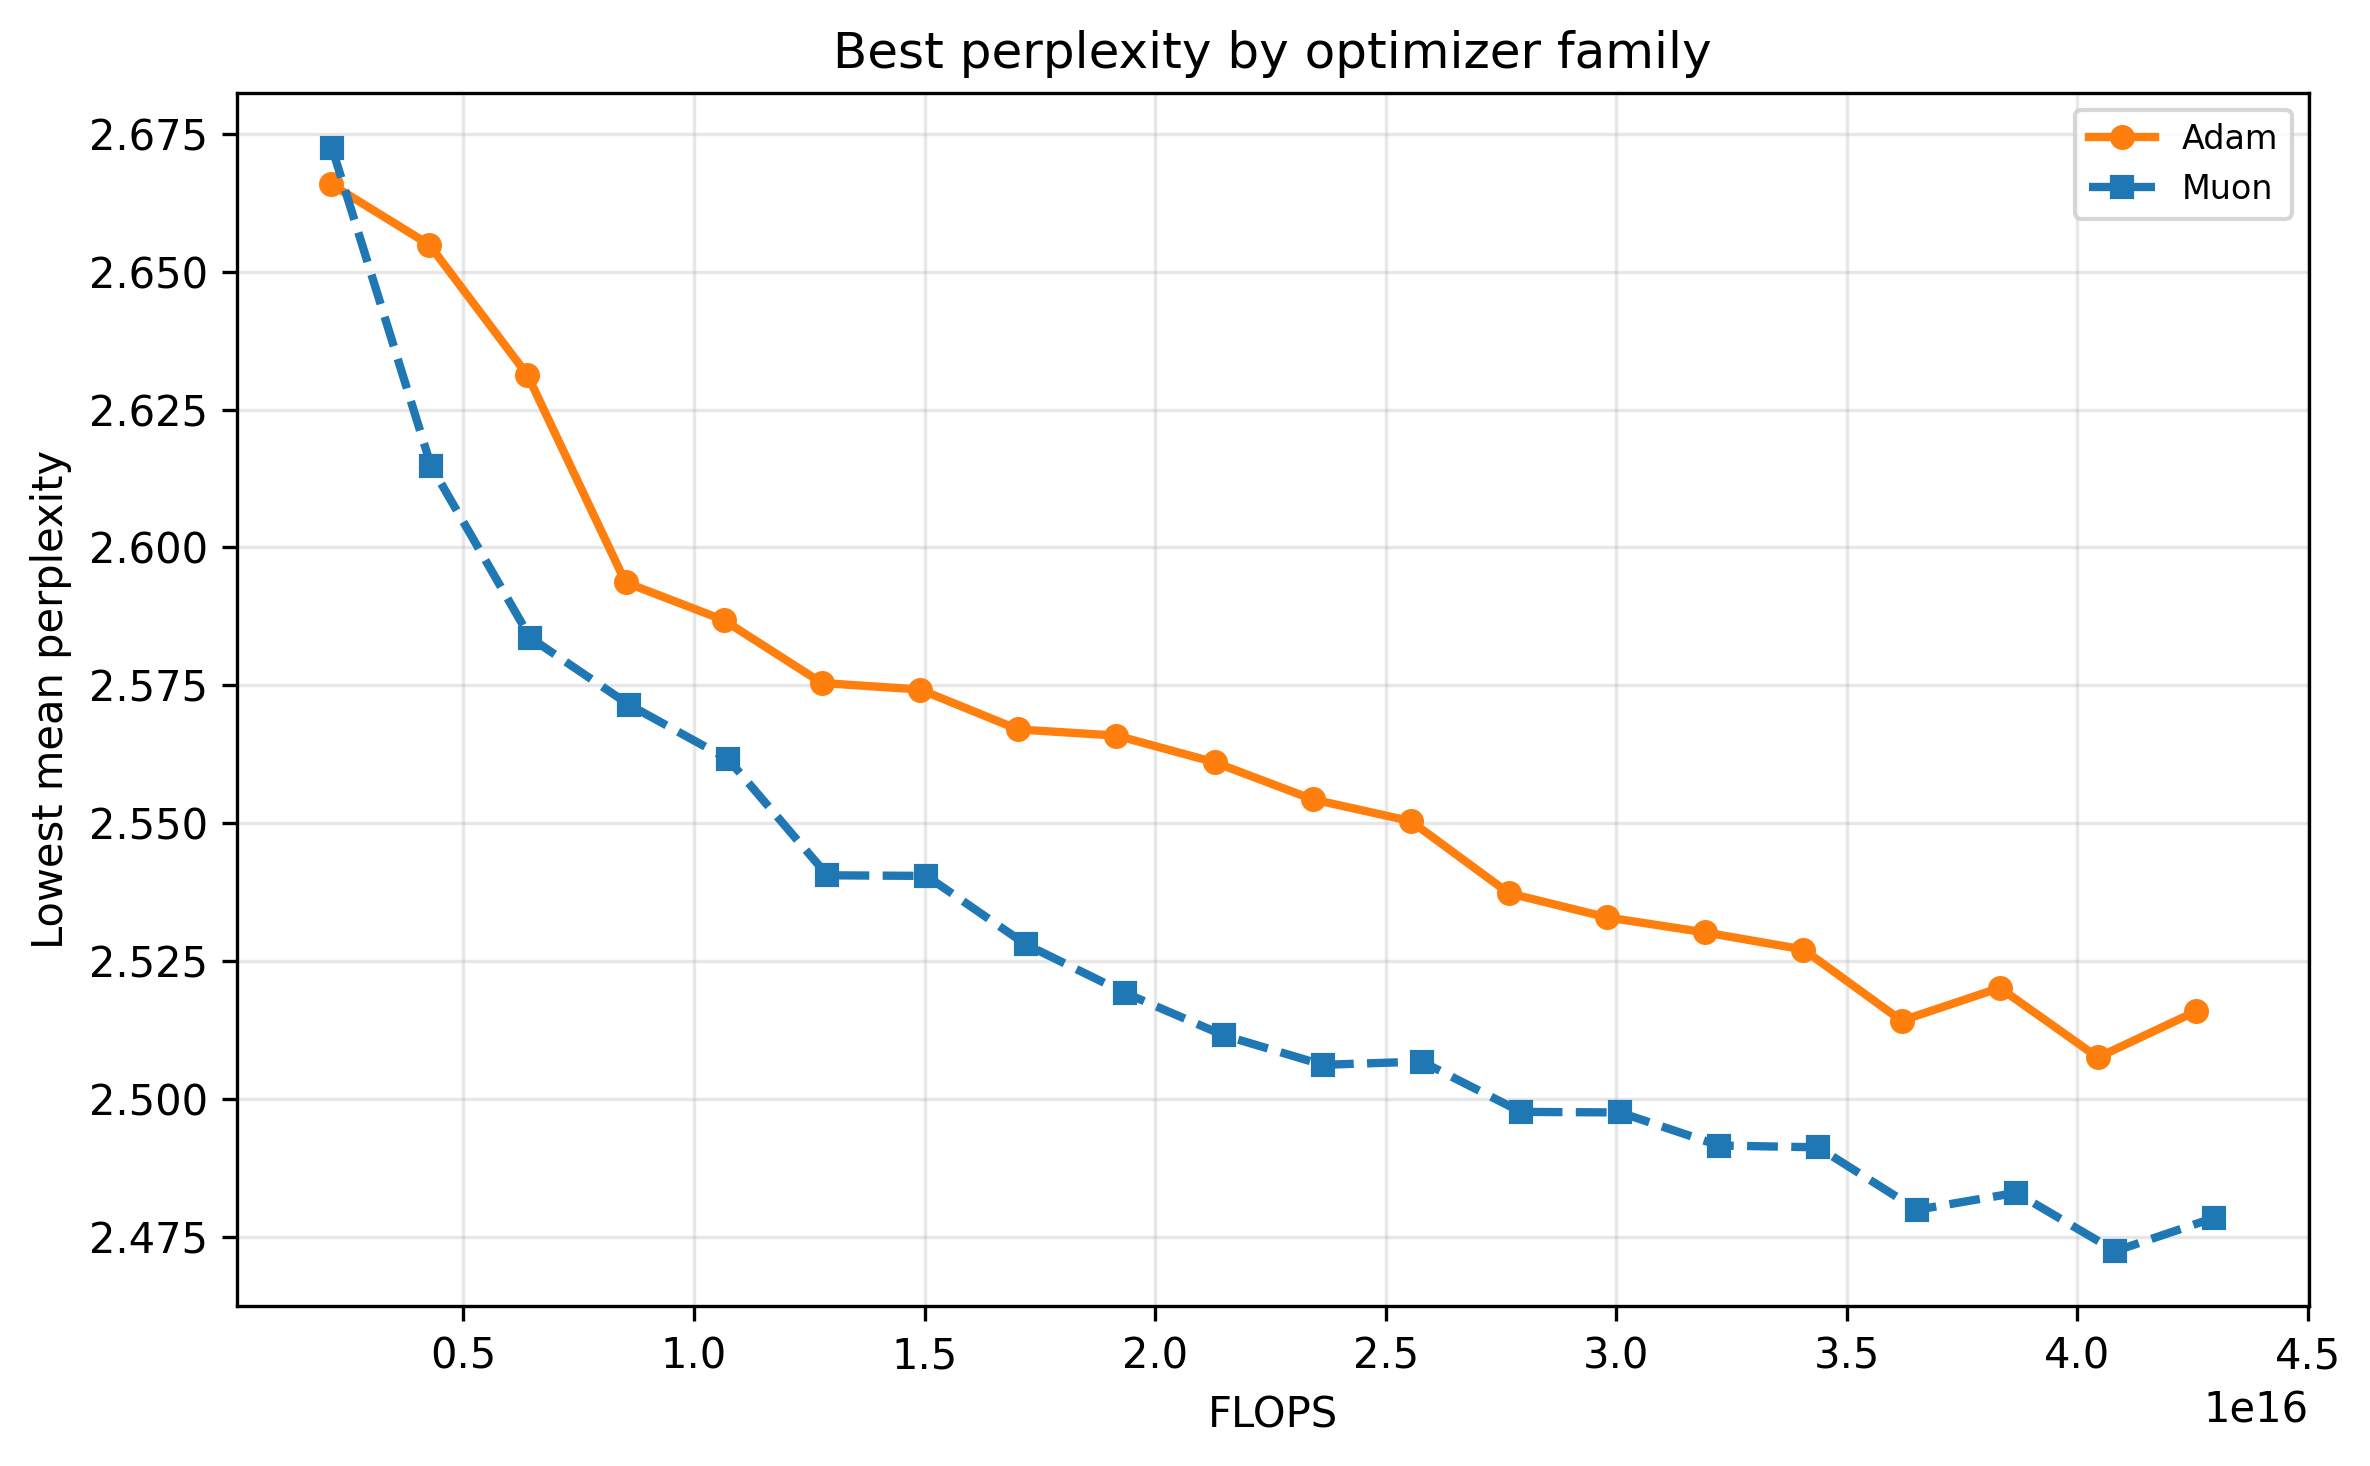
\includegraphics[width=\linewidth]{images/perplexity_best_family_largest_scale_flops.png}
    \caption*{Best family progression by FLOPs}
  \end{subfigure}\hfill
  \begin{subfigure}[t]{0.48\linewidth}
    \centering
    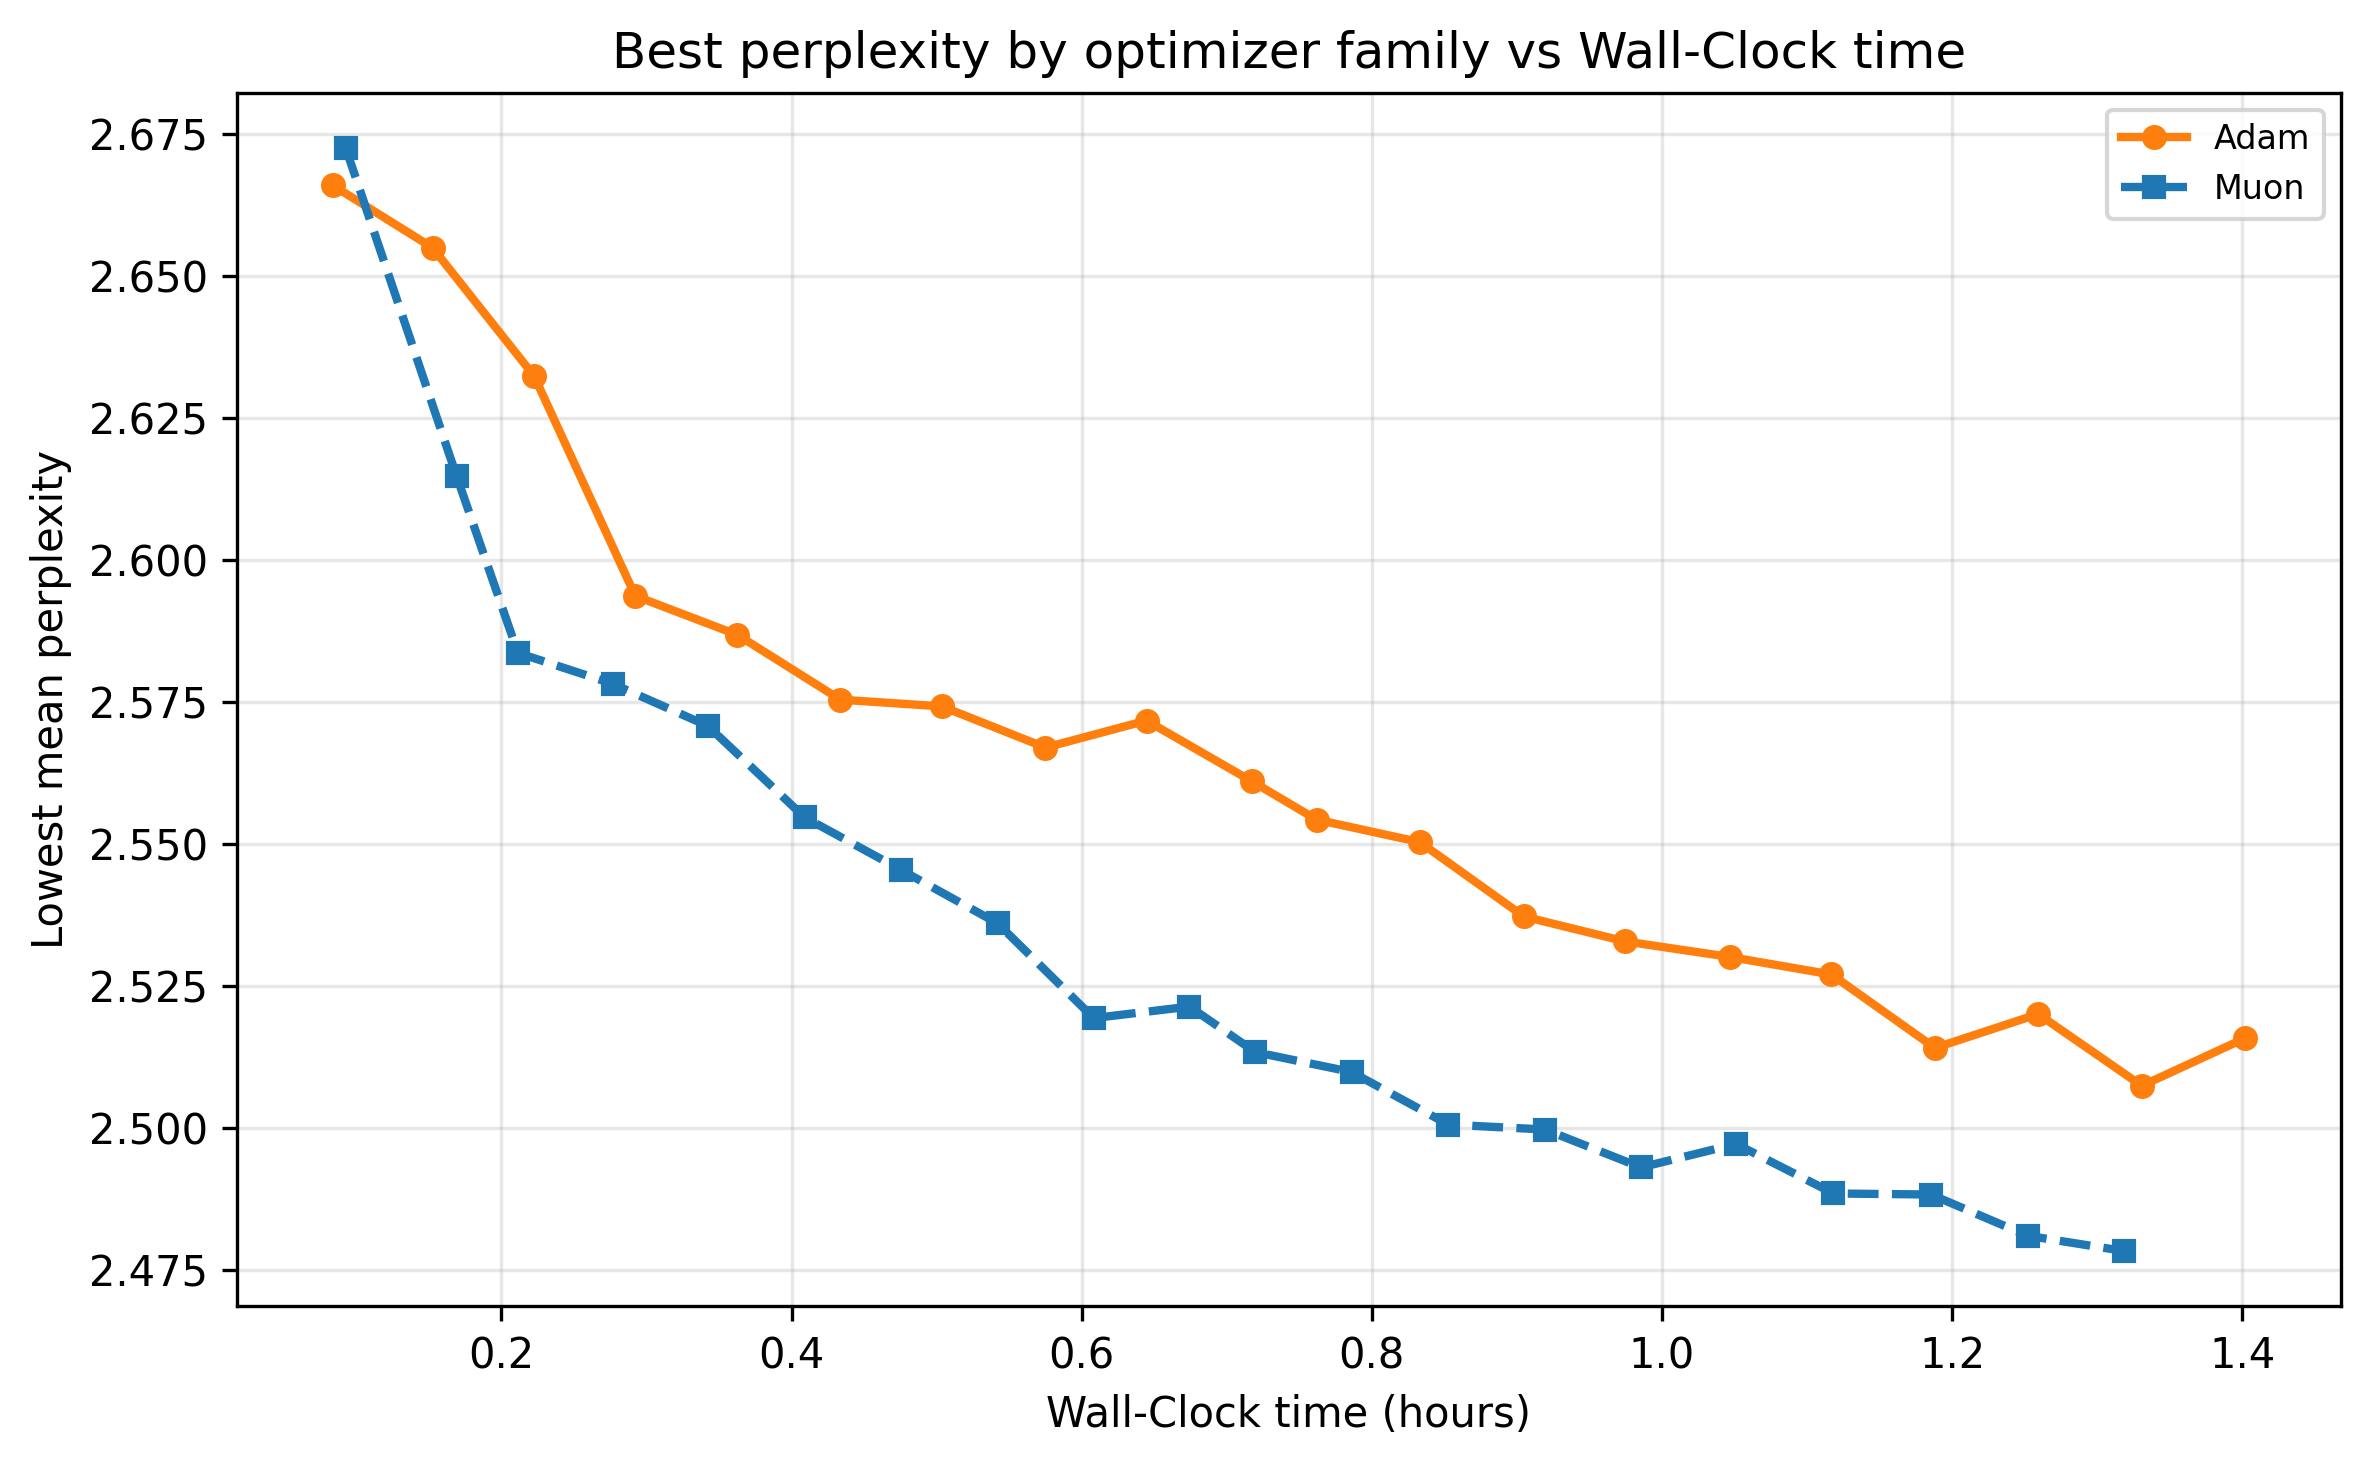
\includegraphics[width=\linewidth]{images/perplexity_best_family_wall_clock_largest_scale.png}
    \caption*{Best family progression by wall-clock time}
  \end{subfigure}
  \caption{Largest-scale family-level progression efficiency.}
  \label{fig:family-progressions}
\end{figure}

The matched-quality advantage plots in Figure~\ref{fig:family-advantages} convert the progression curves into a direct efficiency question: for each Adam perplexity level, how much less compute or wall-clock time does the best Muon run need to reach the same or lower perplexity? Positive values mean Muon reaches the matched target sooner. After the first few matched-perplexity points, Muon's advantage stabilizes rather than appearing as a one-off crossing; across the relevant target range, the FLOP reduction settles around 30--50\%.

\begin{figure}[htbp]
  \centering
  \begin{subfigure}[t]{0.48\linewidth}
    \centering
    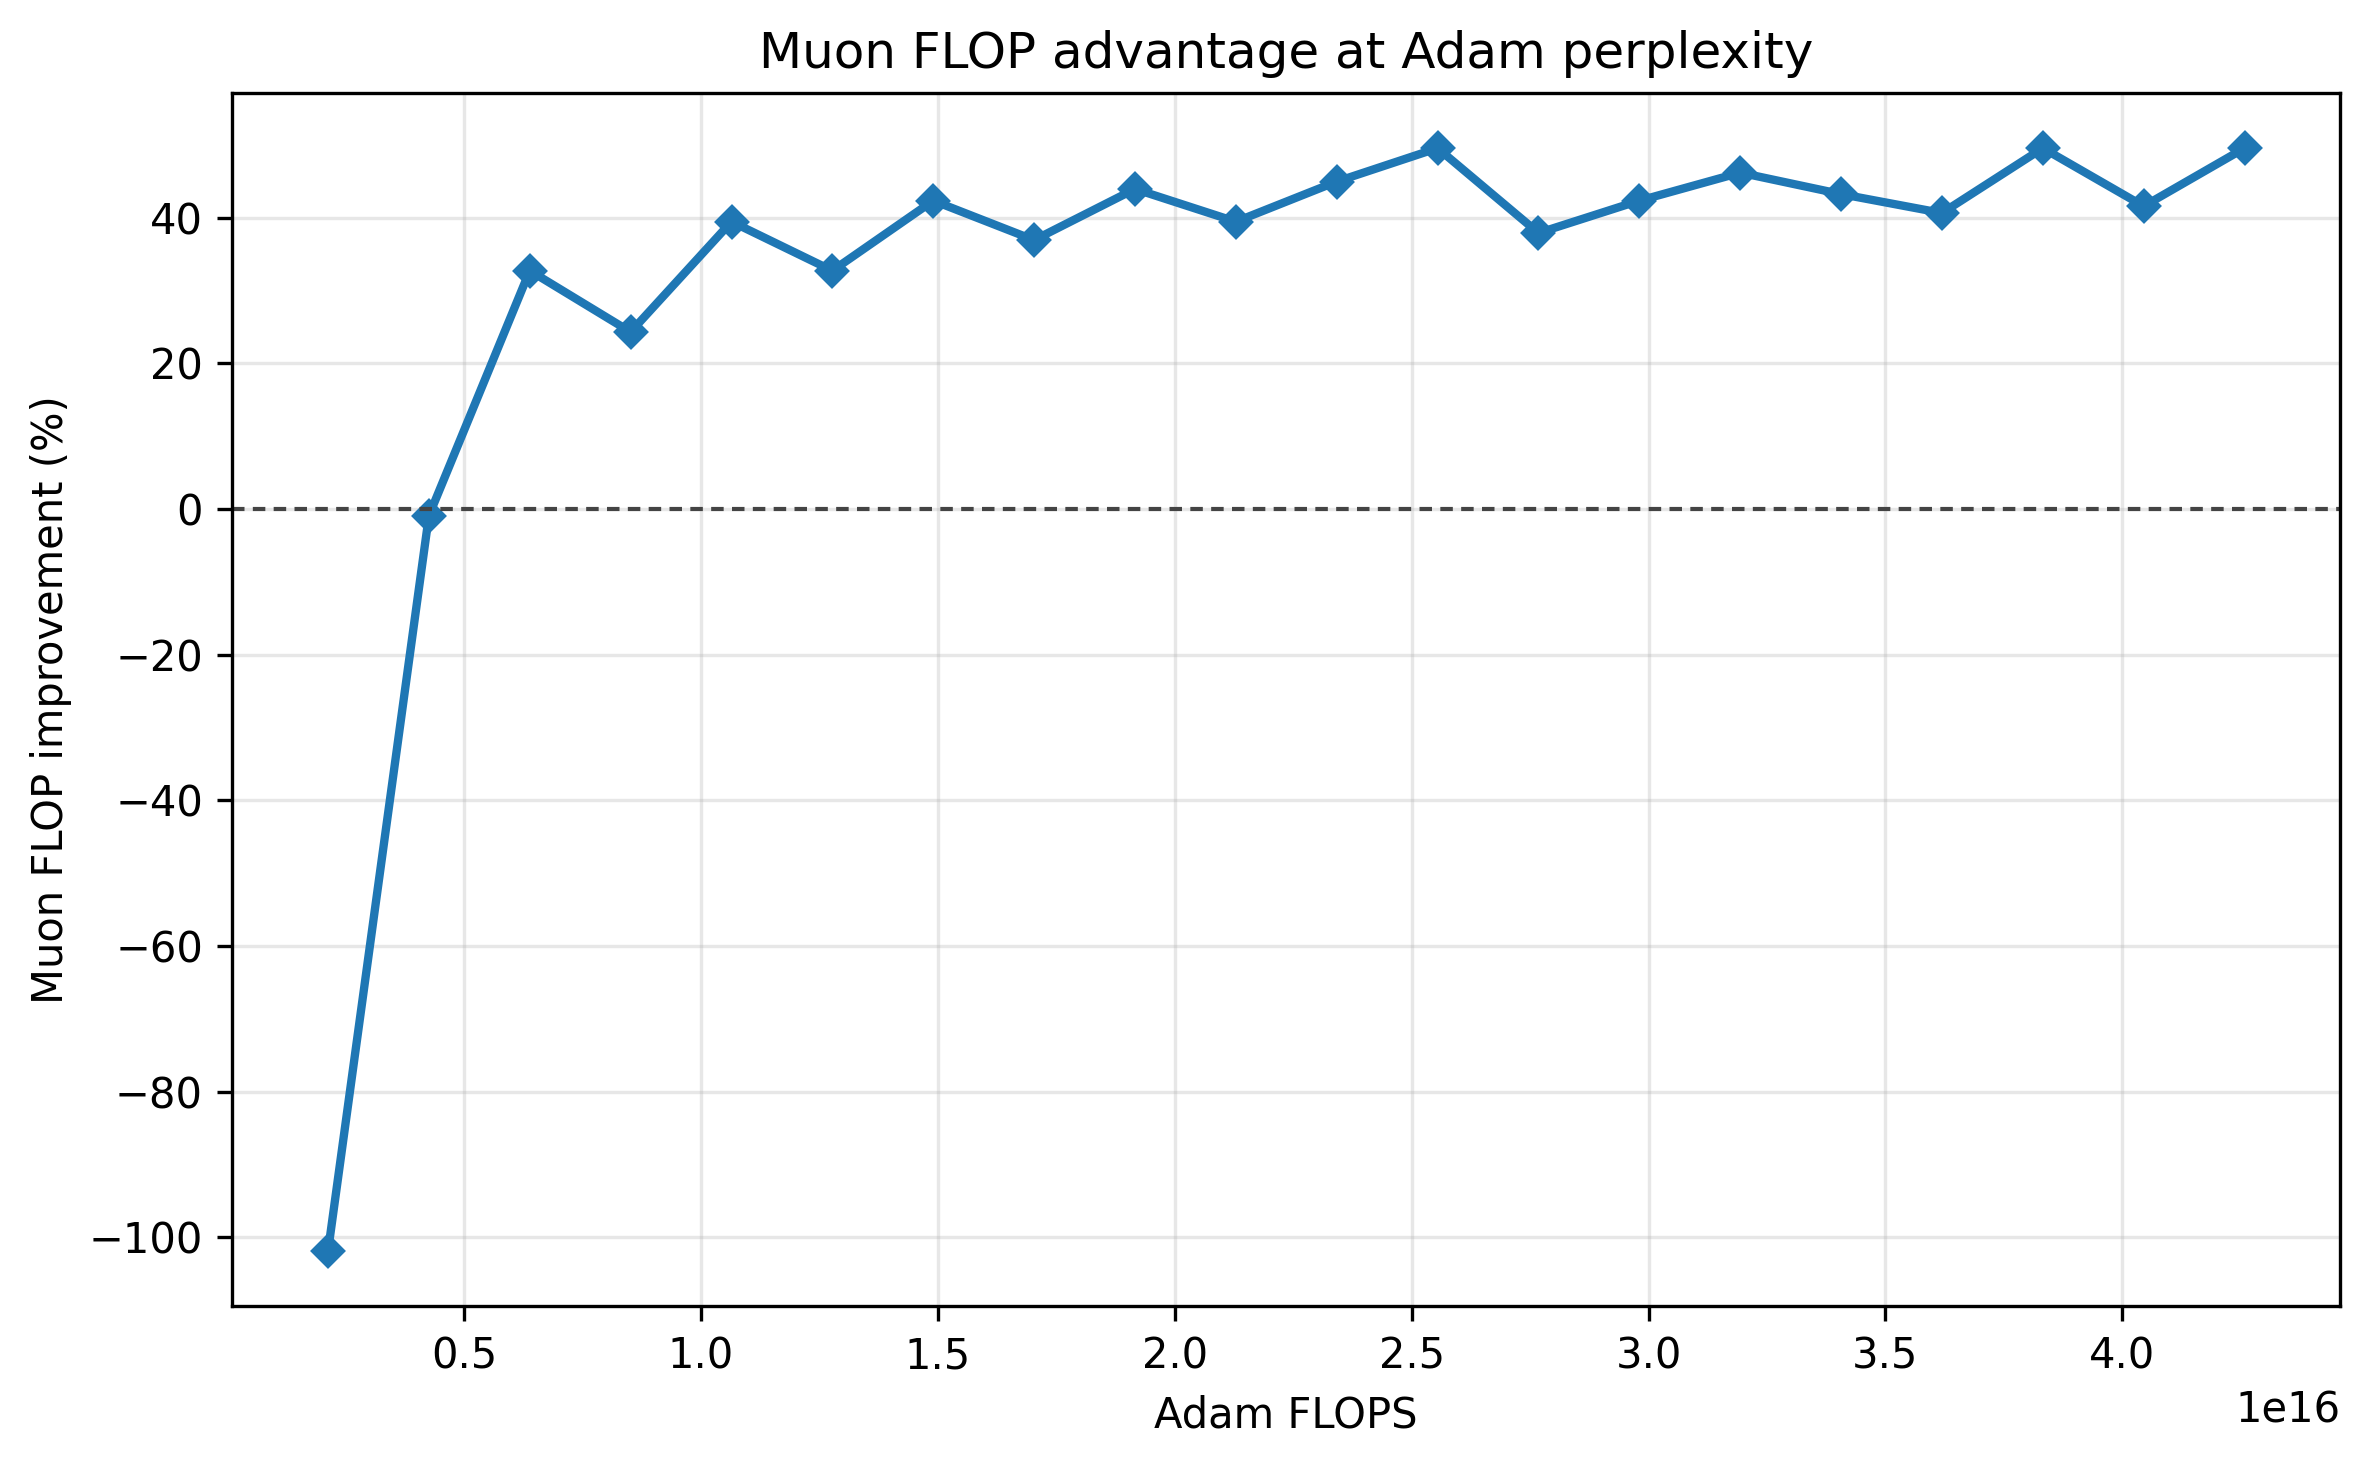
\includegraphics[width=\linewidth]{images/adam_muon_flop_advantage_flops.png}
    \caption*{Matched-perplexity FLOP advantage}
  \end{subfigure}\hfill
  \begin{subfigure}[t]{0.48\linewidth}
    \centering
    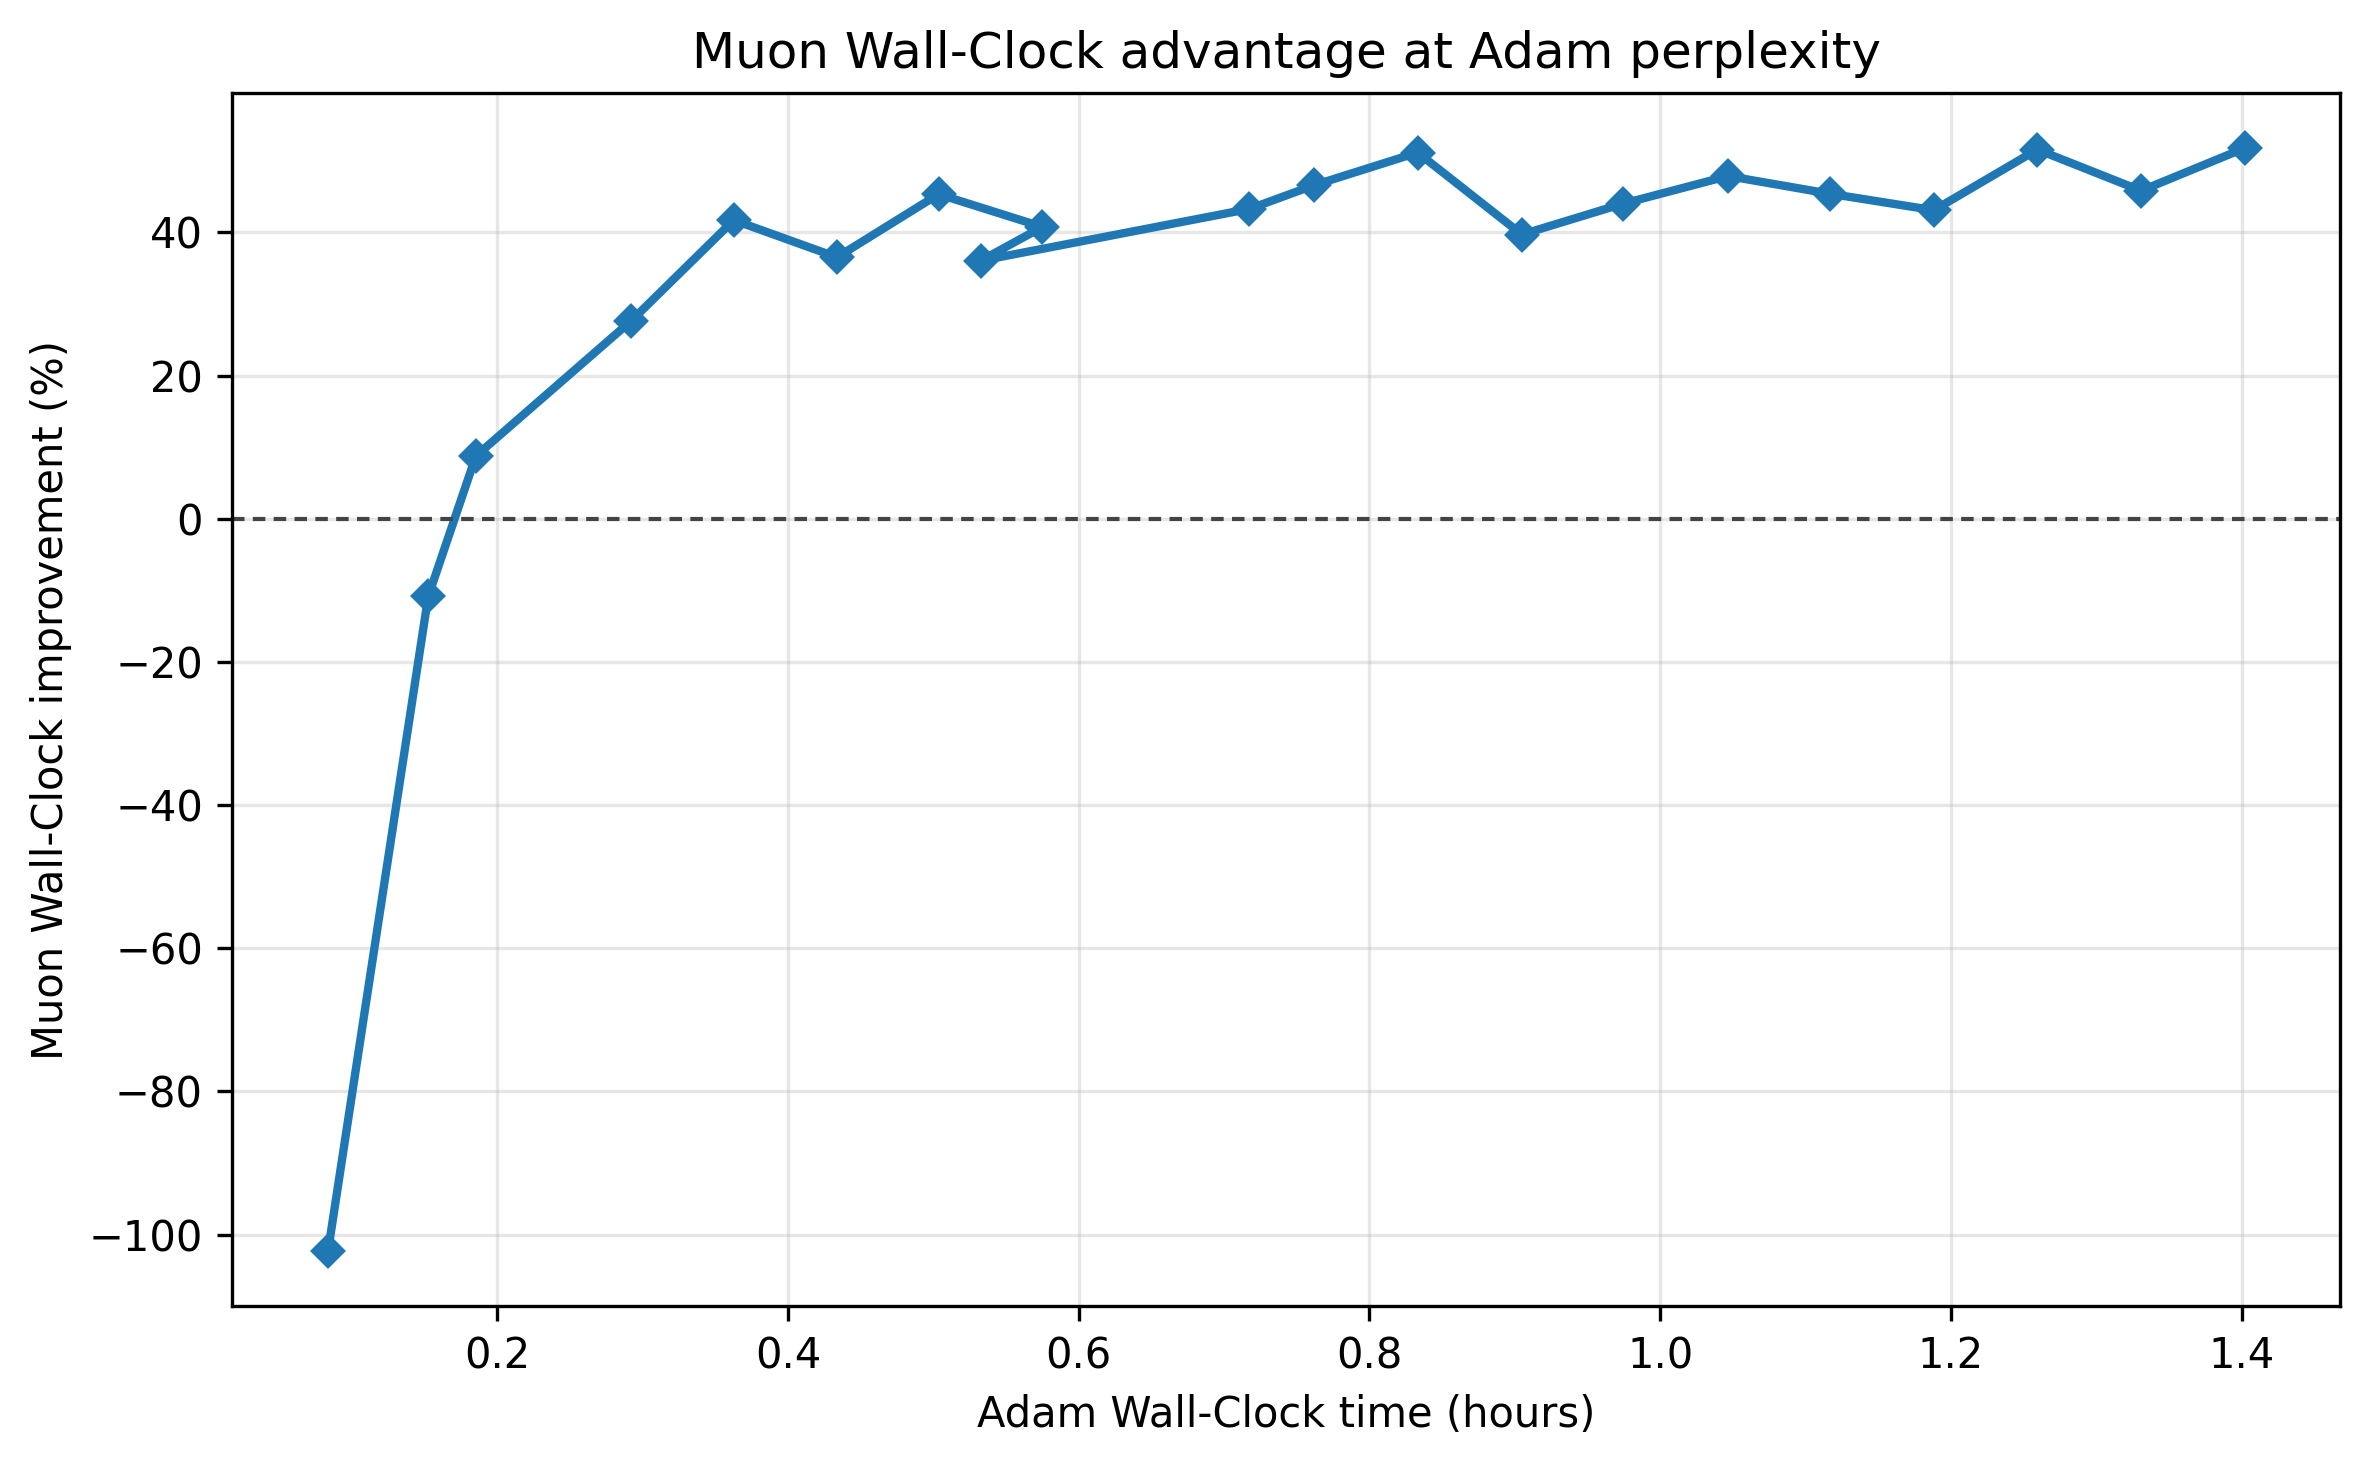
\includegraphics[width=\linewidth]{images/adam_muon_wall_clock_advantage_largest_scale.png}
    \caption*{Matched-perplexity wall-clock advantage}
  \end{subfigure}
  \caption{Muon advantage at matched Adam perplexity.}
  \label{fig:family-advantages}
\end{figure}

\begin{figure}[htbp]
  \centering
  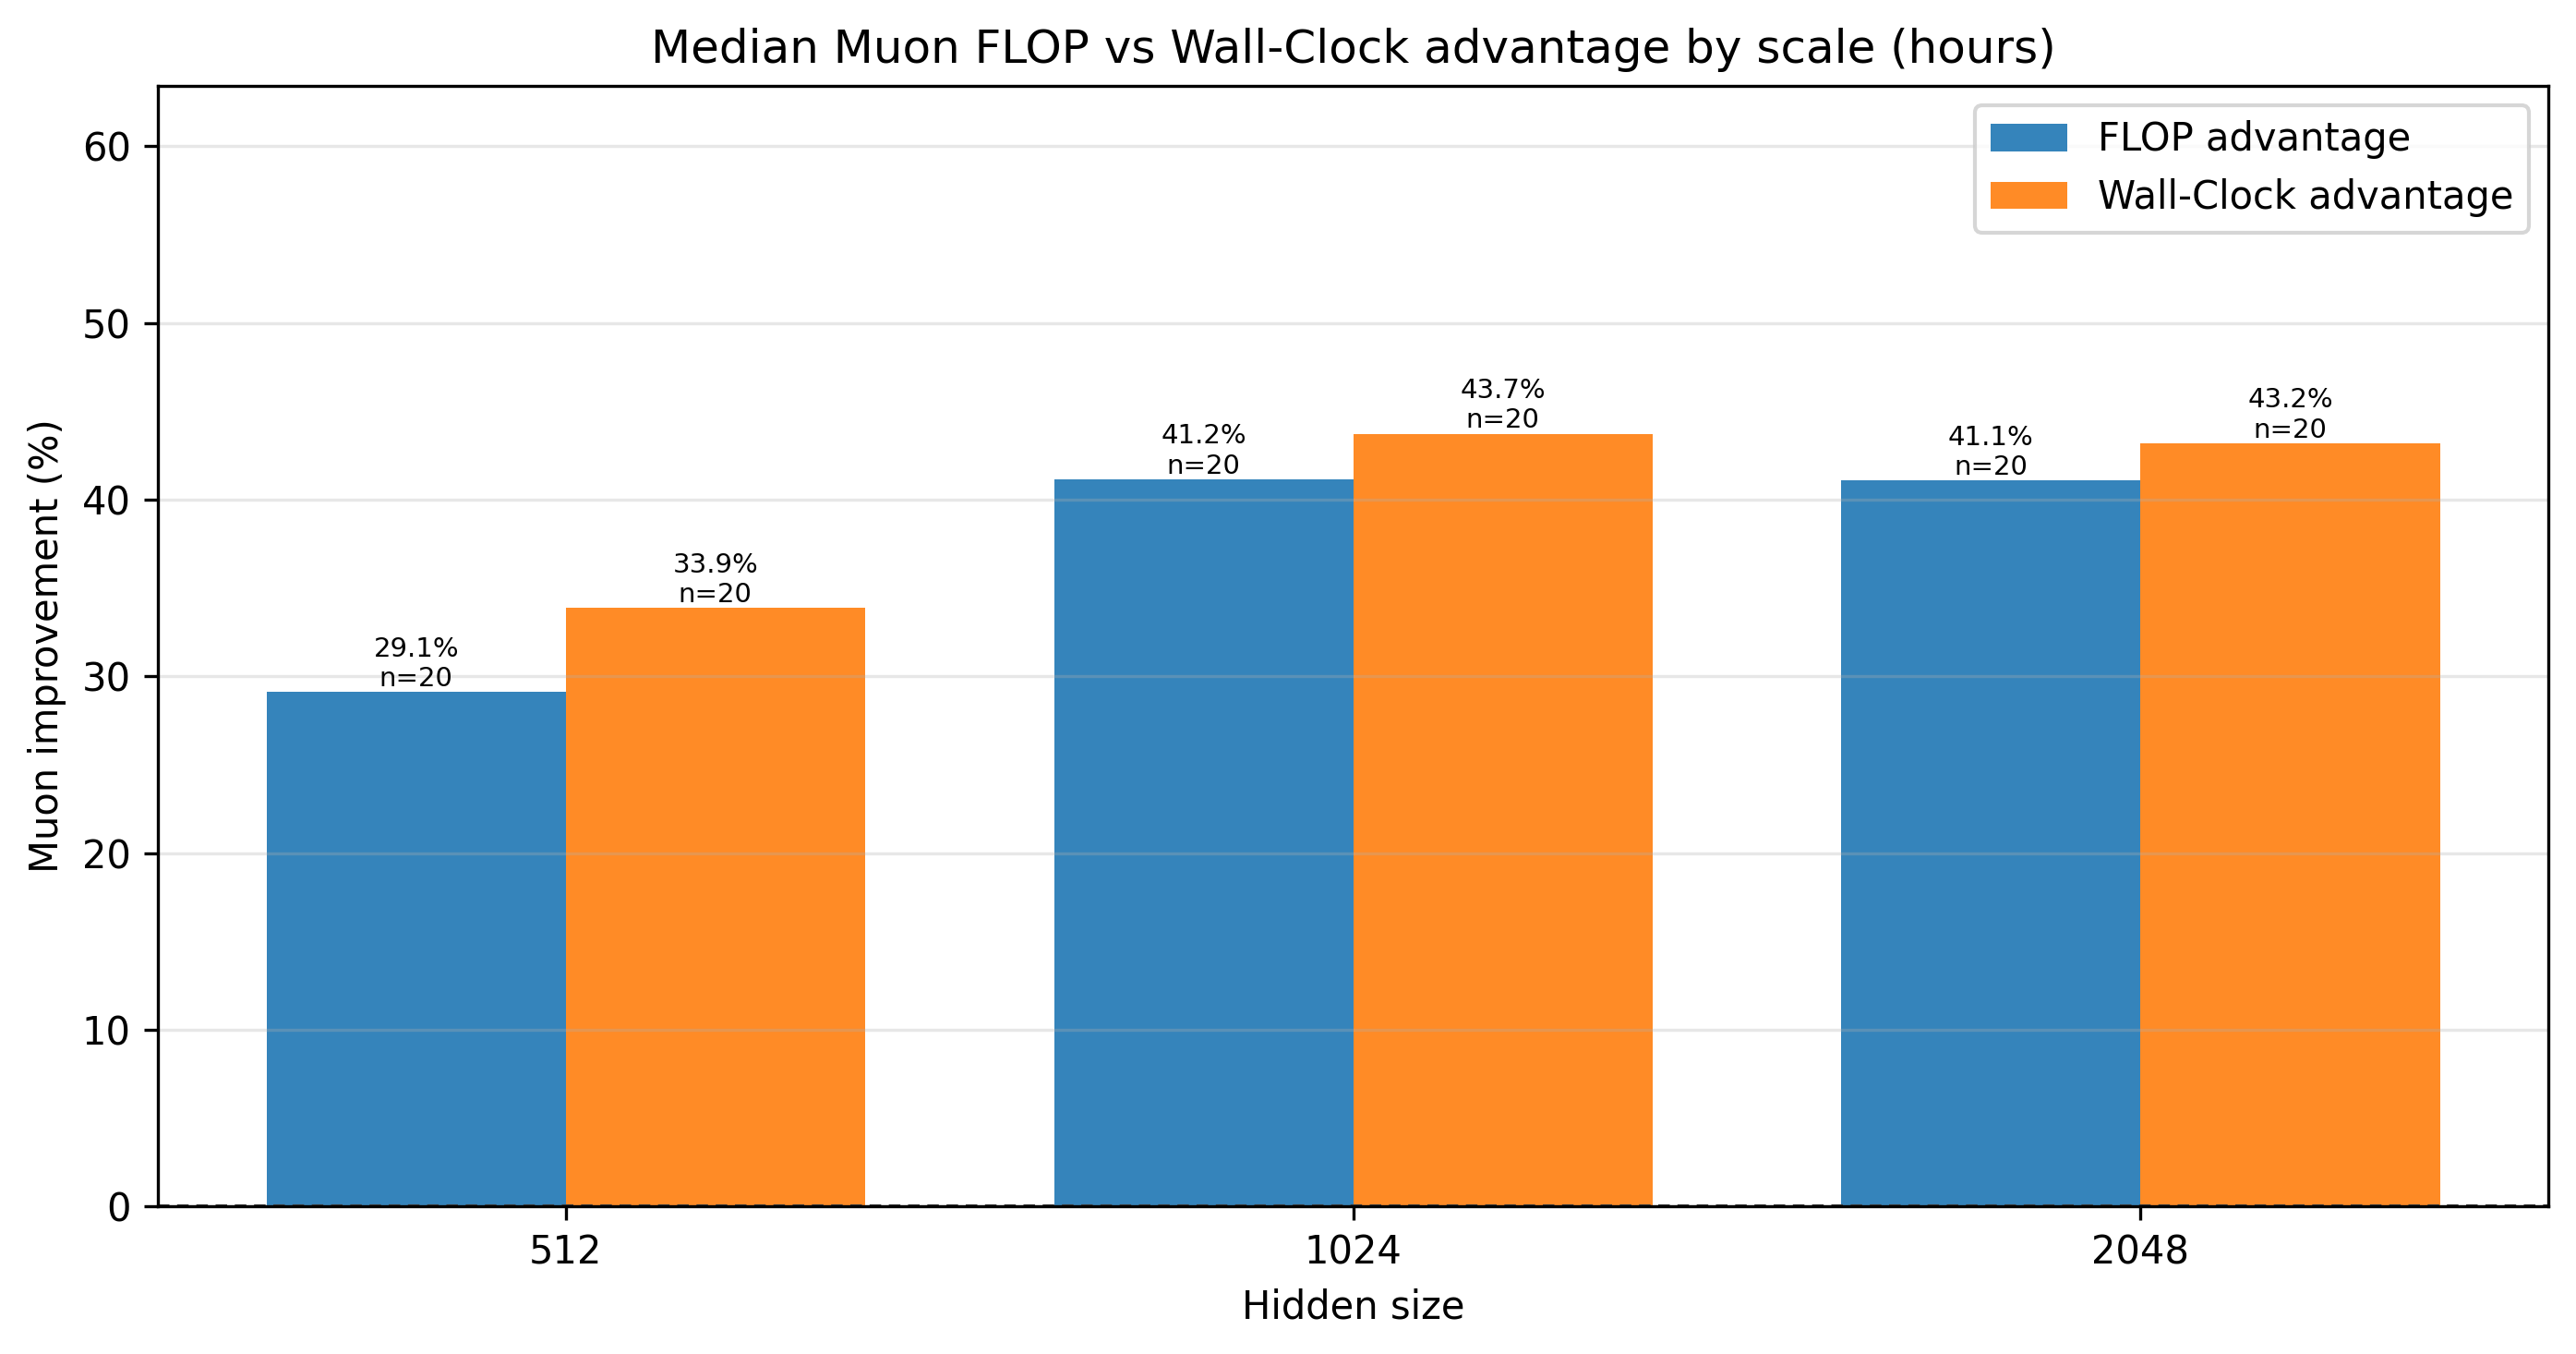
\includegraphics[width=0.85\linewidth]{images/adam_muon_lowest_adam_perplexity_advantage_by_scale.png}
  \caption{Muon FLOP and wall-clock advantage at each scale's lowest Adam perplexity.}
  \label{fig:scale-advantages}
\end{figure}

Muon reaches target quality substantially earlier than the best Adam configuration. Using the lowest Adam perplexity in Figure~\ref{fig:final-perplexity} from the best Adam run at checkpoint 19, the best Muon run crosses the same threshold by checkpoint 13. That is a savings of $6/19 \approx 31.6\%$ of the training steps. Our FLOP axis includes both forward/backward compute and optimizer-step overhead ; the latter is small at this scale, so the step savings translate almost directly into approximately 31.6\% fewer training FLOPs.

\subsection{Test perplexity across sweep grid}

Comparing MuonW and AdamH directly, they are relatively comparable at smaller widths and lower-to-mid learning rates, but MuonW separates more clearly at higher learning rates and larger widths (Figures~\ref{fig:cross-optimizer-heatmap}--\ref{fig:cross-optimizer-sweep}). This scaling trend is important because optimizer choice matters more, not less, as the model moves toward the regime where training compute dominates iteration cost.

\begin{figure}[htbp]
  \centering
  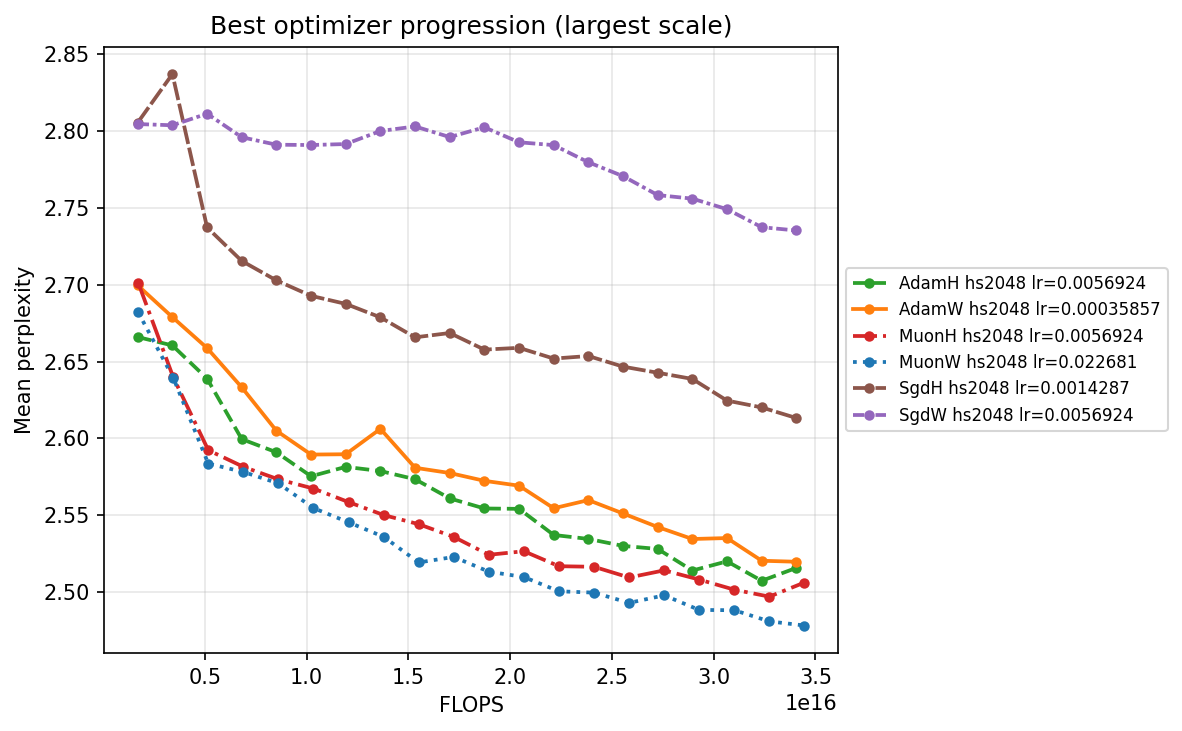
\includegraphics[width=0.85\linewidth]{images/perplexity_best_optimizer_progression_largest_scale_flops.png}
  \caption{Largest-scale optimizer progression.}
  \label{fig:final-perplexity}
\end{figure}

Figure~\ref{fig:final-perplexity} shows mean test perplexity over training FLOPs for the strongest largest-scale configurations from each optimizer variant. Lower perplexity indicates superior probability mass placement on the target DNA sequence. The FLOP conversion uses a base forward/backward term proportional to $6PBL$ per step, plus a per-optimizer update term; for the largest setting, Muon's Newton--Schulz update adds only about $1.17\%$ overhead relative to the base forward/backward pass (Appendix~\ref{app:flops}). The optimizer-level view includes SGD as a baseline and shows a clear separation: SGD remains far above the Adam and Muon curves, Adam improves steadily, and the best Muon configuration reaches its lowest perplexity on a smaller compute budget. The full per-learning-rate and per-optimizer progression curves are provided in Figures~\ref{fig:perp-by-lr-1}--\ref{fig:perp-by-optimizer-muon}.

\subsection{Norm control changes the optimizer ranking}

Hyperball does not uniformly improve both optimizers, and MuonW is the strongest configuration in the present sweep. The interesting failure mode is that Hyperball and Muon seem to want opposite things from the spectrum. Muon whitens the update, trying to spread learning signal across singular directions; Hyperball then projects the whole matrix back to a fixed Frobenius radius by multiplying every singular value by the same scalar.

That uniform projection is harmless if the useful spectrum is already concentrated, but it can be hostile to Muon's attempt to keep small directions alive. Hyperball maps $W_{t+1}=R(W_t+U_t)/\|W_t+U_t\|_F$, so every singular direction is scaled by the same factor. Large singular values survive because they already occupy most of the fixed energy budget $\sum_i\sigma_i^2=R^2$, while smaller singular values are repeatedly pulled back before they accumulate. In this view, MuonH is not simply ``Muon plus better norm control''; it is Muon with a constraint that may erase the very directions Muon is trying to open.

\begin{figure}[htbp]
  \centering
  \makebox[\linewidth][c]{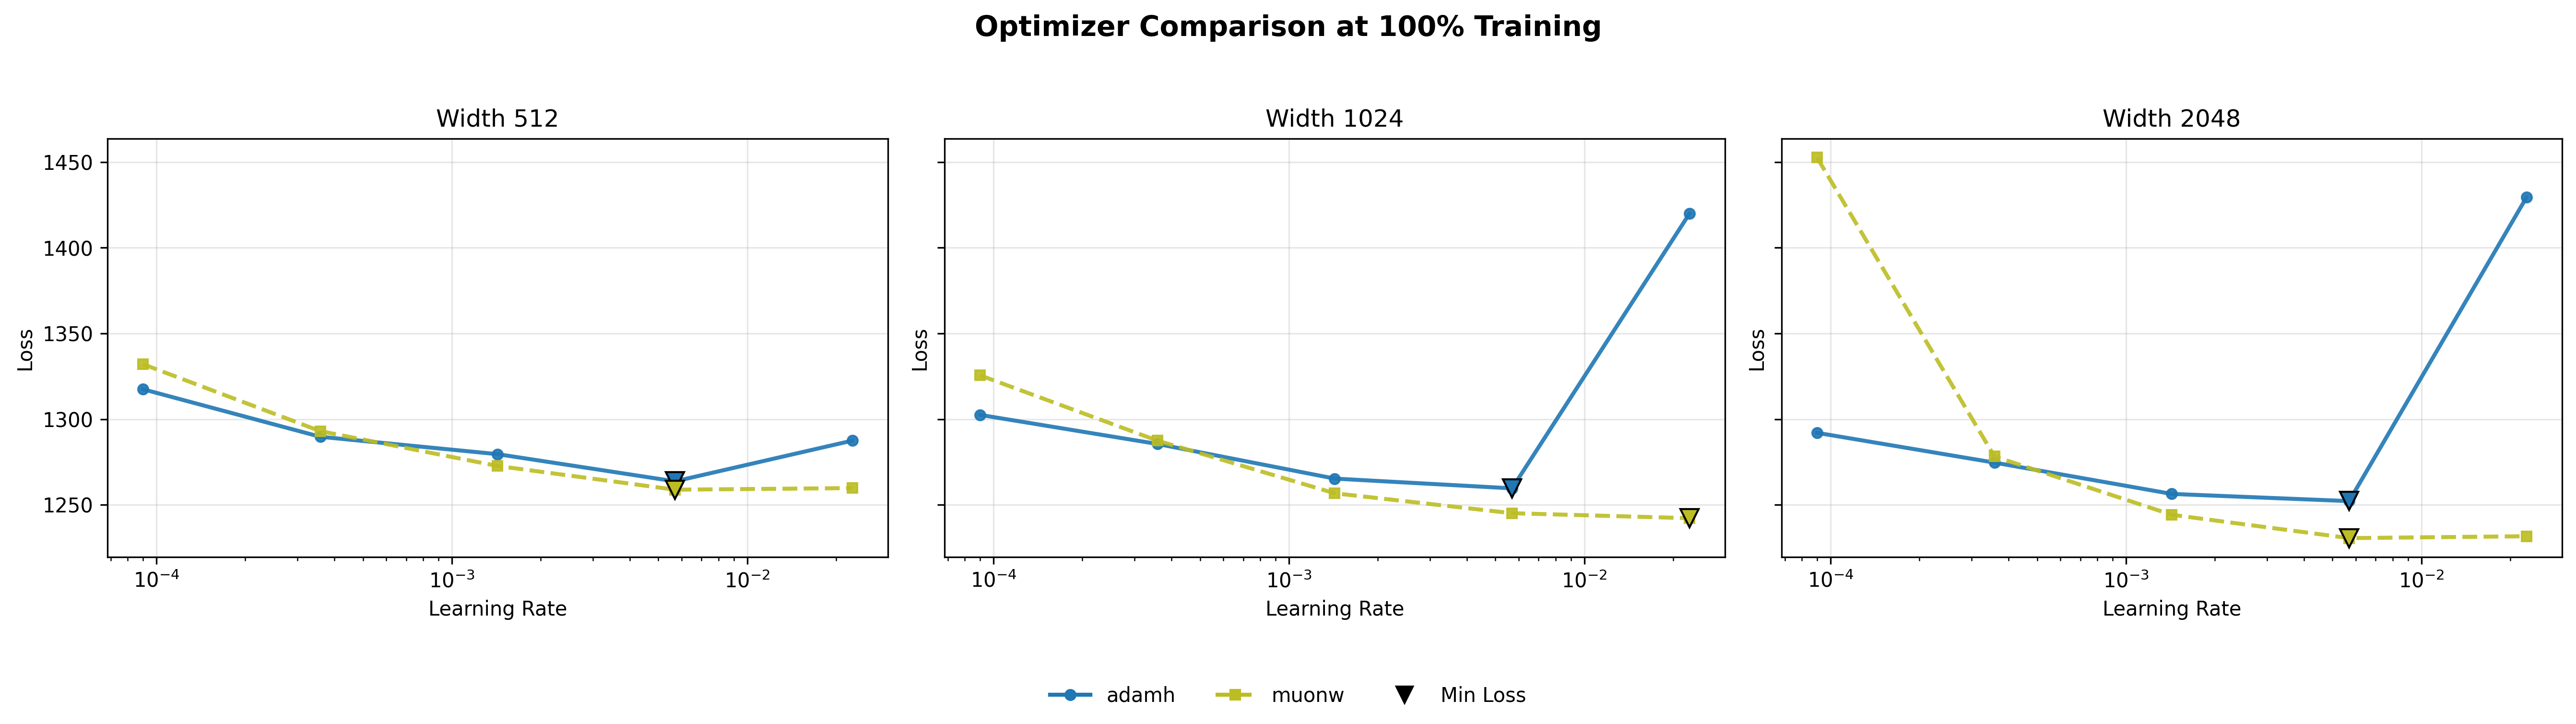
\includegraphics[width=1.06\linewidth]{images/muonw_adamh_comparison.png}}
  \caption{MuonW--AdamH training-loss sweep.}
  \label{fig:muonw-adamh-sweep-loss}
\end{figure}

At the end of training, MuonW becomes strongest toward the higher-learning-rate side of the grid, while AdamH is more competitive in the lower-to-mid range.

% ============================================================
\section{Training dynamics}
\label{sec:training}
% ============================================================

\begin{figure}[htbp]
  \centering
  
\includegraphics[width=\linewidth]{images/loss_curves_nucleotide_loss.png}
  \caption{Training-loss diagnostics.}
  \label{fig:loss-curves}
\end{figure}

Figure~\ref{fig:loss-curves} shows learning curves for the perplexity-selected runs for all four optimizer combinations, with nucleotide cross-entropy loss on the vertical axis.

Consistent with existing literature~\citep{muon,hyperball}, Muon reaches lower training loss than Adam in the runs shown here. The diagnostic ranking matches the main result: MuonW converges fastest, followed by MuonH, AdamH, and AdamW.

The training-loss sweep adds one nuance to the perplexity result. MuonW's lowest-loss region is closer to $\sim 5.69 \times 10^{-3}$ than to the perplexity-selected $\sim 2.27 \times 10^{-2}$, but the two MuonW training losses are nearly tied. We therefore treat training loss as a diagnostic rather than the selection rule: the main claim is about held-out perplexity and FLOPs-to-target, while this loss view only shows that the larger MuonW learning rate does not buy its perplexity result by obviously dominating every training-loss slice.

\subsection{Learning-rate sweep trends}

The sweep loss curves and advantage heatmaps are shown in Figures~\ref{fig:sweep-losses-adam}--\ref{fig:cross-optimizer-sweep}. AdamH is most competitive in a mid-range learning-rate window, whereas AdamW is more stable at the ends. For Muon, MuonH is competitive at smaller learning rates, while MuonW improves toward the upper end.

Across optimizers, the same pattern becomes more pronounced with width. MuonW and AdamH are relatively close at smaller widths and lower-to-mid learning rates, but MuonW gains a clearer advantage at higher learning rates and larger widths. This is the useful interpretation of the learning-rate sweep: Muon's best region shifts upward in learning rate, and that high-learning-rate region becomes more valuable as scale increases.

% ============================================================
\section{Spectral Analysis}
\label{sec:spectral}
% ============================================================

To investigate why Muon with independent weight decay (MuonW) outperforms its constrained counterpart (MuonH) in this sweep, we examine the spectral properties of the learned representations. Following the eigenspectral framework of NerVE~\citep{nerve}\footnote{NerVE originally applies these metrics to track activation dynamics through FFN layers, but the same spectral measures are equally well defined for weight matrices.}, we track two key metrics for the weight matrices:
\begin{itemize}
  \item \textbf{Spectral Entropy:} A measure of how uniformly variance is distributed across singular values. Values near $1.0$ indicate a ``full rank'', diverse representation, while values near $0$ indicate rank collapse.
  \item \textbf{Participation Ratio (PR):} The effective rank of the matrix. We normalize the PR to get the ratio of the effective rank to full rank.
\end{itemize}

\begin{figure}[htbp]
  \centering
  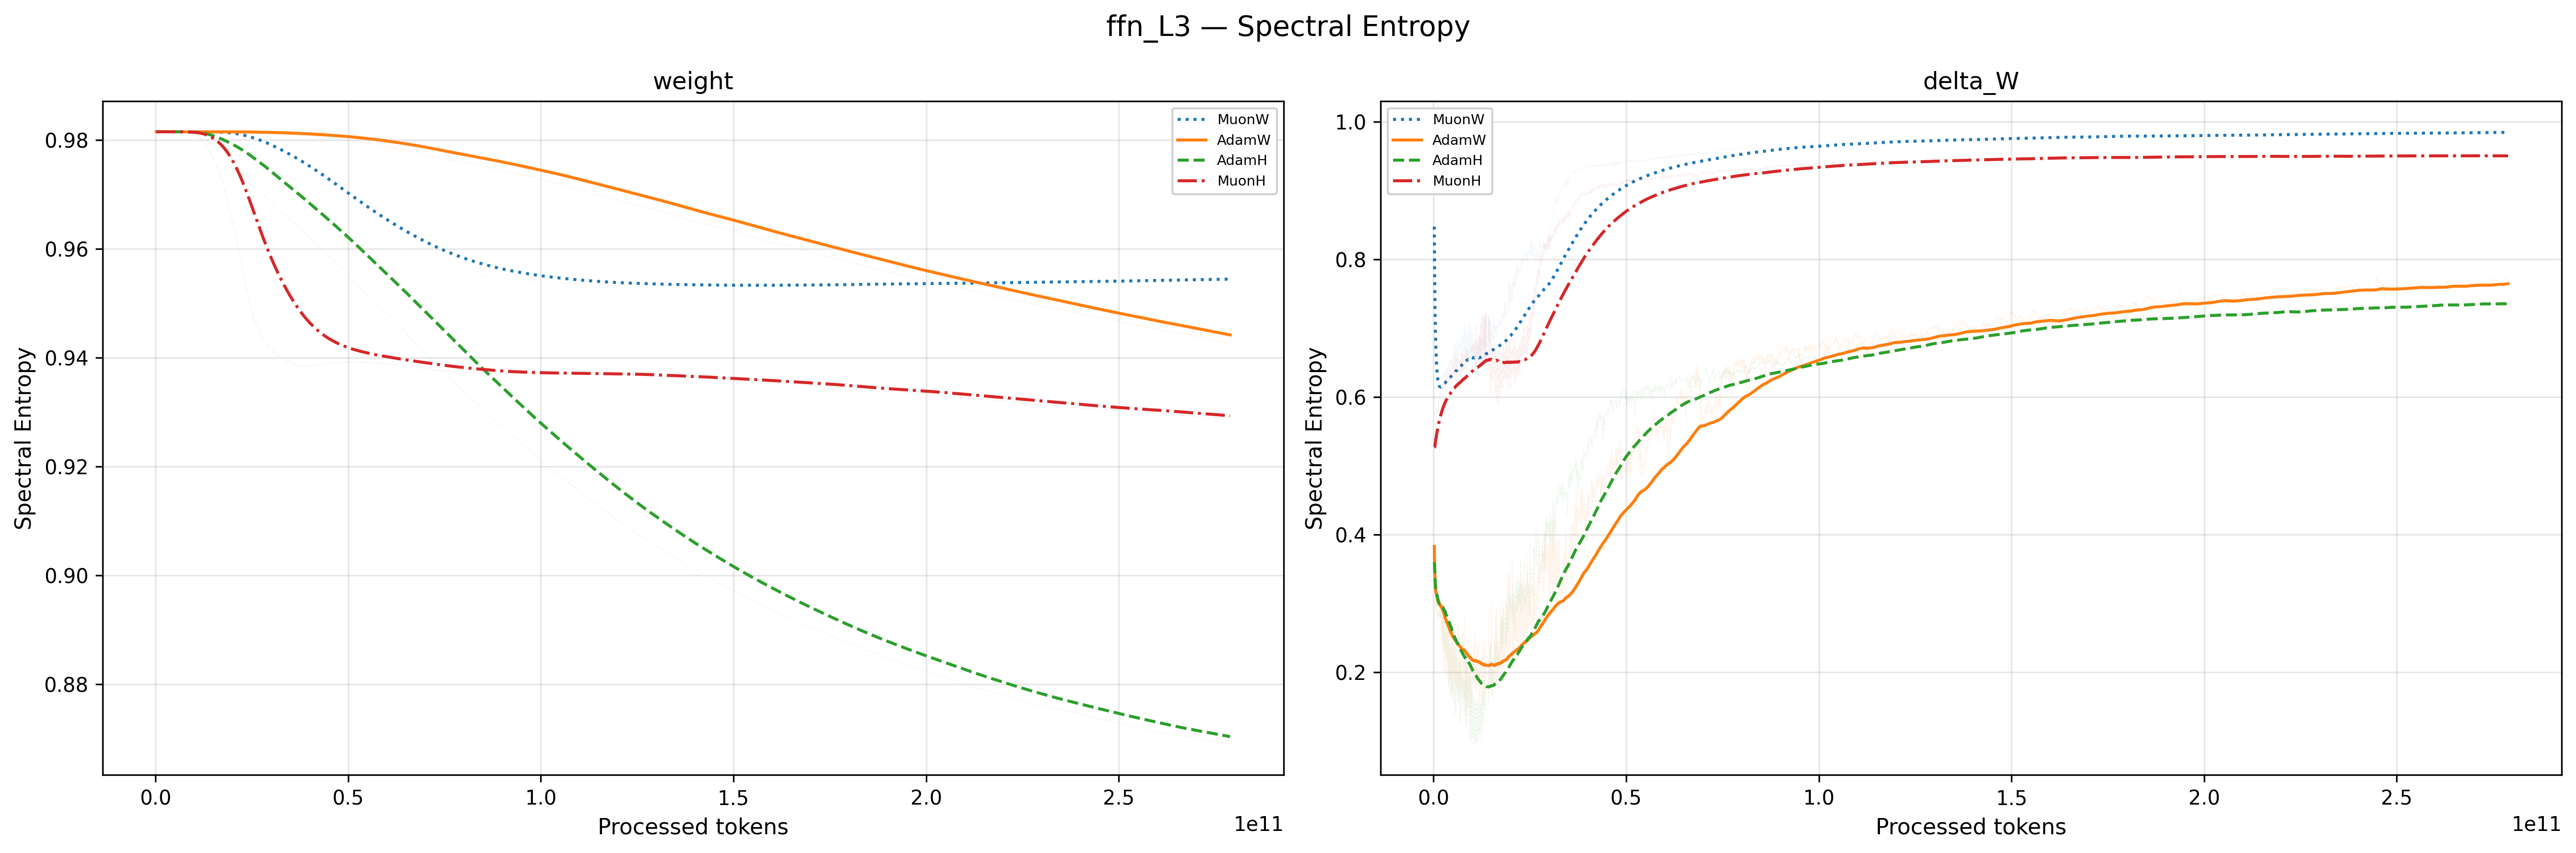
\includegraphics[width=\linewidth]{images/svd_entropy_mean_ffn_L3.png}\\[0.85em]
  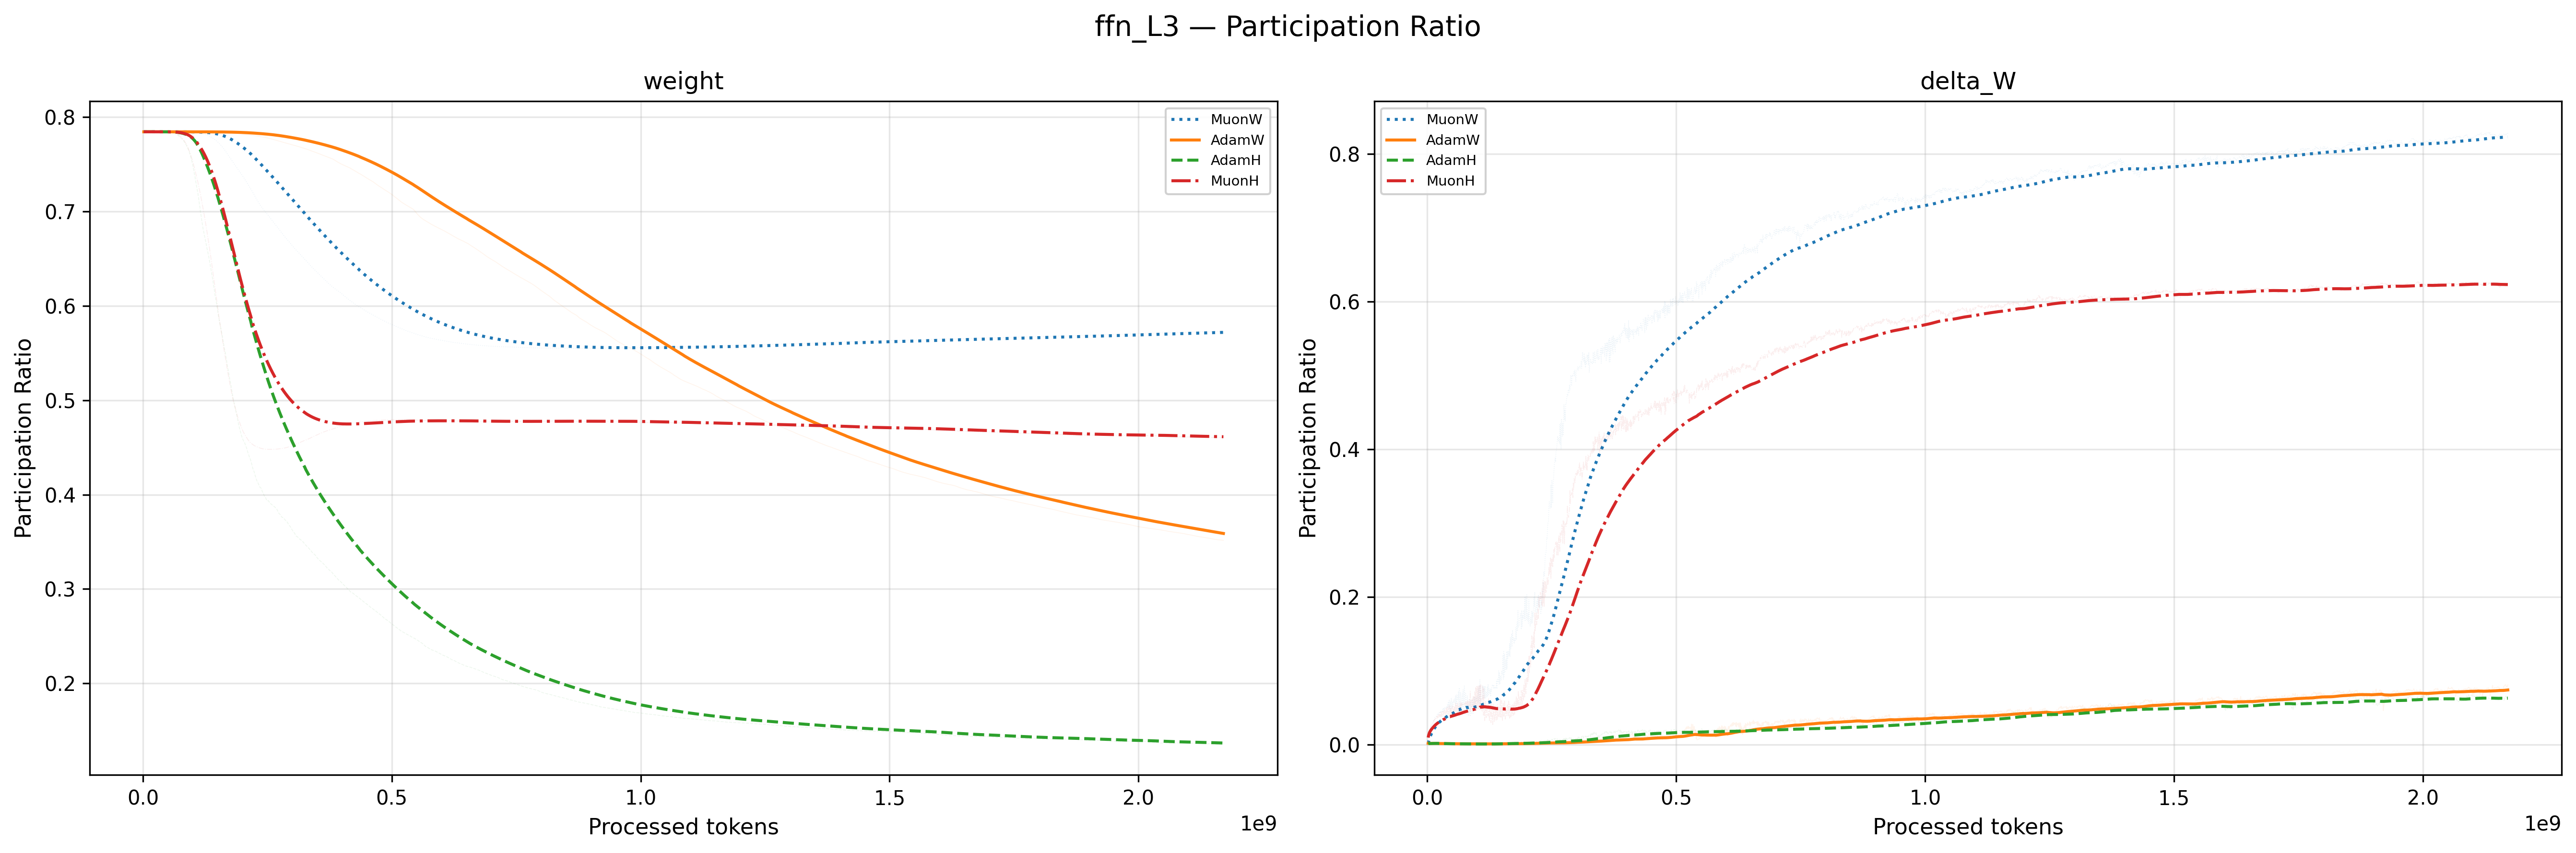
\includegraphics[width=\linewidth]{images/pr_mean_ffn_L3.png}
  \caption{Spectral metrics for FFN Layer~3. Top: Spectral Entropy. Bottom: Participation Ratio. \textbf{Blue:} MuonW, \textbf{Red:} MuonH, \textbf{Orange:} AdamW, \textbf{Green:} AdamH.}
  \label{fig:spectral}
\end{figure}

MuonW and MuonH start with similarly high spectral entropy ($\approx 0.98$), but they diverge sharply. MuonW stays near $\approx 0.93$, while MuonH falls to $\approx 0.68$ and its participation ratio drops in tandem (Figure~\ref{fig:spectral}). Since both use the same Muon whitening, this divergence is consistent with the Hyperball constraint contributing to rank collapse~\citep{repdeg}. Muon's whitening is not perfectly full-rank in practice: five Newton--Schulz iterations push singular values toward $1$ rather than exactly to $1$, near-zero singular values in the momentum matrix remain hard to revive, and independent weight decay means the actual $\Delta W$ also includes a $-\lambda W_t$ term. All weight matrices exhibited similar patterns; we show only one here for simplicity.

\subsection{Uniform Rescaling and the Spectral Squeeze}

MuonH constrains $\|W\|_F = R$ at every step by uniformly rescaling all singular values. A plausible consequence is that weak directions are repeatedly pushed down before they accumulate, concentrating the spectrum into fewer dominant modes.

This may be compounded by imperfect whitening on the update side. Muon's 5-step Newton--Schulz iteration only approximately whitens the update, so if the weight spectrum becomes increasingly anisotropic under Hyperball, the update can inherit that bias instead of correcting it.

MuonW has no such hard rescaling step and maintains substantially higher spectral entropy and participation ratio throughout training. AdamW also maintains relatively high entropy compared with AdamH and MuonH, but likely through a different mechanism: coordinate-wise updates can keep smaller singular directions active through noisier per-parameter adaptation, whereas MuonW does so through matrix-whitened updates that deliberately spread signal across directions. This distinction matches the broader NerVE view that stable spectral signatures track optimizer design choices~\citep{nerve}.

\subsection{Implicit Annealing and Relative Step Size}

\begin{figure}[htbp]
  \centering
  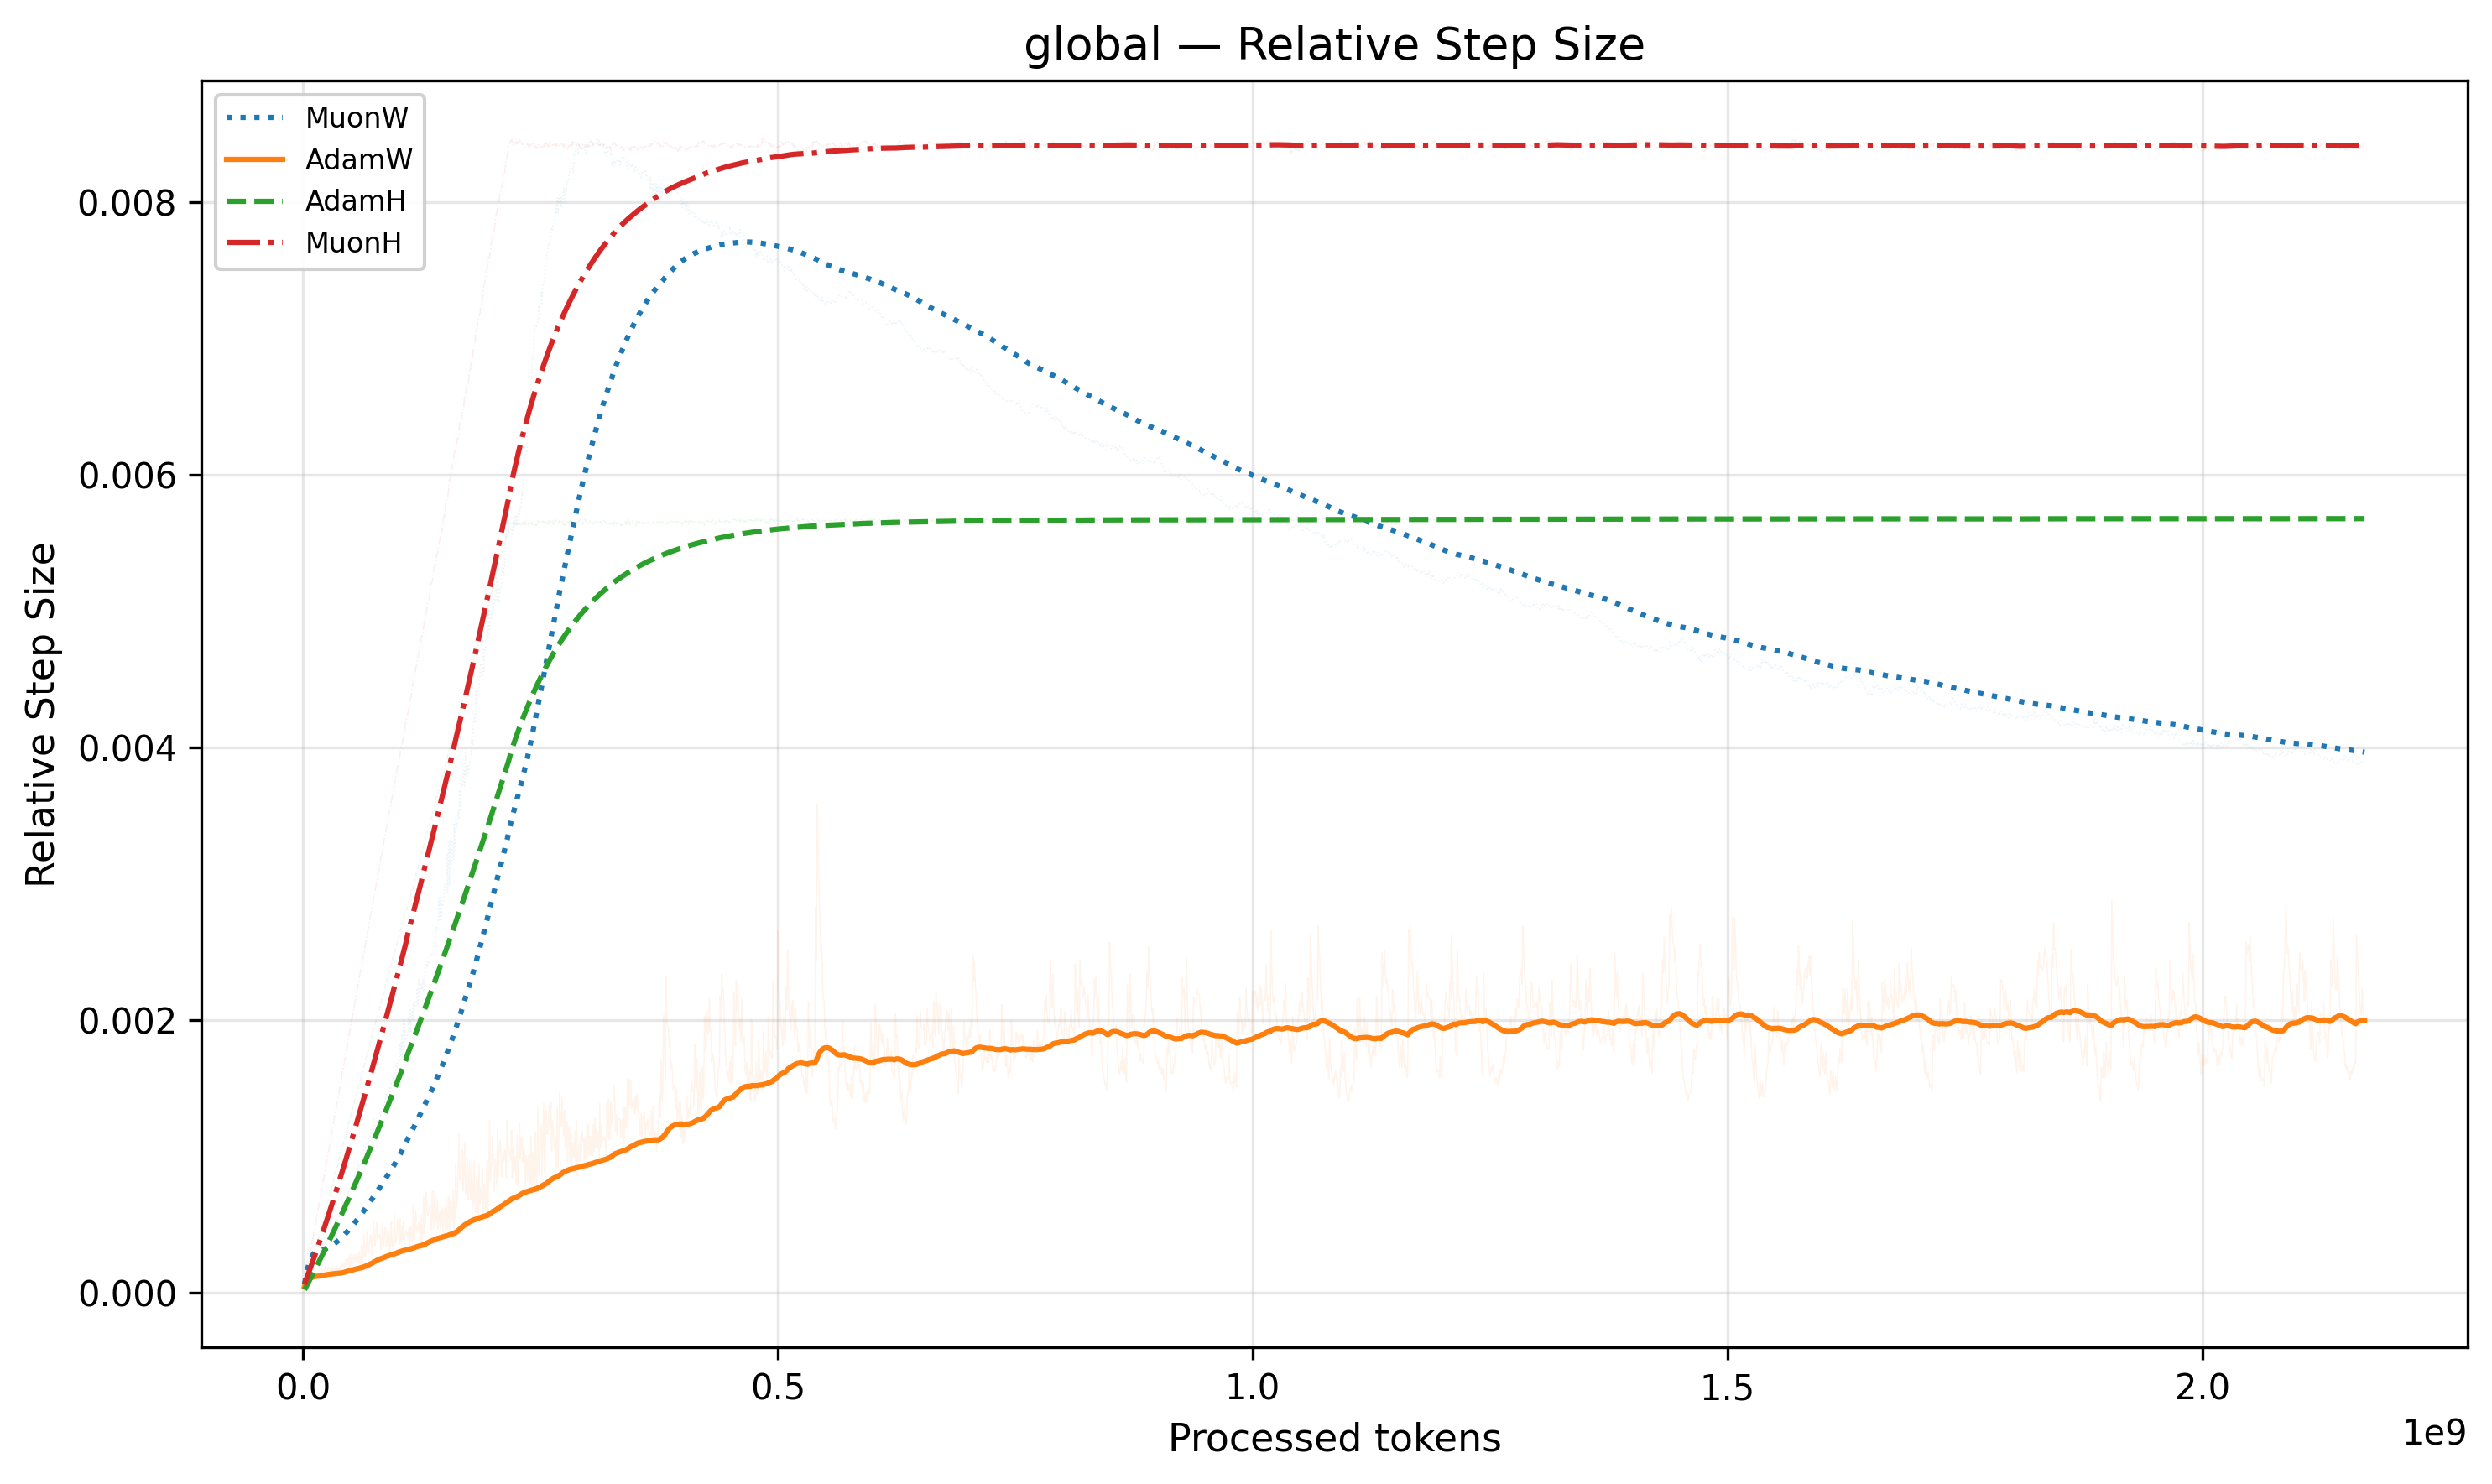
\includegraphics[width=0.9\linewidth]{images/relative_step_size.png}
  \caption{Relative step size.}
  \label{fig:dynamics-stepsize}
\end{figure}

The second piece is the relative step size, $\|\Delta W\|/\|W\|$. MuonW shows a decaying relative step size as the weight norm grows, while MuonH plateaus. The initial ramp-up corresponds to the learning-rate warmup schedule. Under MuonW the weight norm grows over training, so the relative step size decays even when $\|\Delta W\|$ stays roughly constant (Figures~\ref{fig:dynamics-stepsize} and~\ref{fig:dynamics-norms}). This may act like an implicit annealing schedule.

For MuonH, $\|W\|$ is fixed, so the relative step size does not show the same decay. This may limit late-stage refinement.


% ============================================================
\section{Discussion and Conclusion}
\label{sec:discussion}
% ============================================================

Optimizer choice and weight regularization substantially affect the compute efficiency of regulatory DNA training. In our controlled sweep, the best Muon run reaches the best Adam target quality with approximately 31.6\% fewer training FLOPs. Optimizer comparisons also change when norm control is varied explicitly rather than fixed: in this setting, independent weight decay pairs better with Muon than Hyperball, and the best Muon configuration is the most compute-efficient configuration we tested. For models used upstream of costly biological experiments, cheaper model iteration can translate into more budget for candidate screening and validation.

% ============================================================
\section{Limitations}
\label{sec:limitations}
% ============================================================

The results presented here should be interpreted with several limitations in mind:
\begin{itemize}
  \item \textbf{Scope of evaluation:} the study evaluates optimizer behavior primarily through test perplexity and time-to-target FLOPs on a fixed architecture, dataset, and training recipe. The conclusions therefore concern optimization efficiency in this setting, not the full biological utility of the model.
  \item \textbf{Model scale:} the experiments are conducted in a few-hundred-million-parameter regime comparable to AlphaGenome, Enformer, and Borzoi. The relative ranking of optimizers may change at substantially larger scales.
  \item \textbf{Mechanistic interpretation:} the spectral analyses identify mechanisms that are consistent with the observed behavior, but they do not by themselves establish causality. In particular, the roles of norm growth and spectral concentration remain partially confounded.
\end{itemize}


% ============================================================
\clearpage
\appendix
\section*{Appendix}
% ============================================================

\section{Data}
\label{app:data}

\section{Adam Overview}
\label{app:adam}

Let $g_t = \nabla_W \mathcal{L}(W_t)$ denote the gradient at step $t$. Adam maintains two exponential moving averages (EMAs):
\begin{itemize}
  \item a \emph{first moment} estimate (mean) $m_t$,
  \item a \emph{second moment} estimate (uncentered variance) $v_t$.
\end{itemize}
Specifically, with hyperparameters $\beta_1,\beta_2 \in [0,1)$ and initialization $m_0 = 0$, $v_0 = 0$:
\begin{align}
m_t &= \beta_1 m_{t-1} + (1-\beta_1) g_t, \label{eq:adam-m}\\
v_t &= \beta_2 v_{t-1} + (1-\beta_2) g_t^2, \label{eq:adam-v}
\end{align}
where $g_t^2$ denotes elementwise squaring.

Because both EMAs start at zero, they are biased toward $0$ early in training. Adam, therefore, uses bias corrected estimates
\[
\hat m_t = \frac{m_t}{1-\beta_1^t},
\qquad
\hat v_t = \frac{v_t}{1-\beta_2^t}.
\]
The vanilla Adam update is then,
\[
W_{t+1} = W_t - \eta\, \frac{\hat m_t}{\sqrt{\hat v_t}+\varepsilon},
\]
with learning rate $\eta$ and small $\varepsilon > 0$ for numerical stability.

\paragraph{Weight decay (AdamW).}
Soft L2 regularization can be implemented by adding $\lambda W_t$ to the gradient, but AdamW instead \emph{decouples} weight decay from the adaptive gradient step. In its common form:
\[
W_{t+1} = (1-\eta\lambda)\,W_t \; - \; \eta\, \frac{\hat m_t}{\sqrt{\hat v_t}+\varepsilon},
\]
so weight decay shrinks parameters directly (multiplicatively), while the Adam step uses the adaptive per-parameter scaling.

\paragraph{Independent weight decay.}
In our setting, we use \emph{independent} weight decay: the shrinkage is applied as a separate step, not through the gradient, and is not tied to the learning rate. Concretely, if $U_t$ denotes the optimizer's proposed parameter update (e.g., the Adam step $U_t=-\eta\, \hat m_t/(\sqrt{\hat v_t}+\varepsilon)$), then independent weight decay applies
\[
W_{t+1} = (1-\lambda)\,W_t + U_t.
\]
So the decay rate $\lambda$ is not multiplied by the learning rate and can be scheduled separately. Throughout the paper, we use AdamW to denote Adam plus this independent weight decay, and MuonW to denote Muon plus this independent weight decay.


\section{SVD Overview}
\label{app:svd}

\paragraph{Singular value decomposition (SVD).}
For any real matrix $A \in \mathbb{R}^{m\times n}$, the SVD factorizes $A$ into
\[
A = U\Sigma V^\top,
\]
where $U\in\mathbb{R}^{m\times m}$ and $V\in\mathbb{R}^{n\times n}$ are orthogonal matrices (their columns form orthonormal bases), and $\Sigma\in\mathbb{R}^{m\times n}$ is diagonal (rectangular) with nonnegative entries $\sigma_1\ge \sigma_2\ge \cdots \ge 0$ called the \emph{singular values}. Geometrically, $V^\top$ rotates (or reflects) the input space, $\Sigma$ scales along the orthogonal axes, and $U$ rotates (or reflects) the output space.

\paragraph{What are singular values?}
The singular values of matrix $A$ are the square roots of the eigenvalues of $A^\top A$. Concretely, for eigenpairs $(\lambda_i, v_i)$ of $A^\top A$,
\[
A^\top A v_i = \lambda_i v_i, \qquad \sigma_i = \sqrt{\lambda_i}.
\]
They quantify how much $A$ \emph{stretches} vectors: along the right singular direction $v_i$, the mapping scales by exactly $\sigma_i$. The largest singular value is the \emph{maximum stretch} induced by $A$ on any unit vector:
\[
\sigma_1 = \max_{\|x\|=1}\|Ax\|.
\]
Note that $\sigma_2$ is the maximum stretch orthogonal to $v_1=\argmax_{\|x\|=1}\|Ax\|$, i.e., $\sigma_2=\max_{x\perp v_1,\,\|x\|=1}\|Ax\|$, and so on\footnote{We can generalize using the min-max theorem: $\sigma_i=\min_{\substack{U\subseteq \mathbb R^n \\ \dim U=n-i+1}}\max_{\substack{x\in U \\ \|x\|=1}}\|Ax\|$.}.

\paragraph{Why are they special?}
They control several important properties at once:
\begin{itemize}
  \item \textbf{Spectral norm/stability:} The spectral norm is defined as $\|\cdot\|_2=\sigma_1(\cdot)$ on matrix inputs. It is the operator norm\footnote{Formally, the operator norm $\|\cdot\|_p$ is defined for $A\in \mathbb R^{m\times n}$ as $\|A\|_p=\max\{\|Ax\|_p:x\in \mathbb R^n, \|x\|_p\le 1\}$, where we apply the $\ell_p$ norm to the vectors.} induced by the vector $\ell_2$ norm. $\sigma_1(A) = \|A\|_2$ is the maximum amplification (or stretch) of $A$; this is important for Lipschitz bounds~\citep{spectral}.
  \item \textbf{Rank / effective dimension:} the number of nonzero $\sigma_i$ equals $\mathrm{rank}(A)$; many tiny $\sigma_i$ indicates a nearly low rank map.
  \item \textbf{Conditioning:} the ratio $\sigma_1/\sigma_r$ (for $\sigma_r = \min_{\neq 0}\sigma_i$) measures how unevenly $A$ scales different directions; large ratios can hurt optimization and numerical stability.
\end{itemize}


\section{Muon Overview}
\label{app:muon}

While Adam~\citep{adam} (see Appendix~\ref{app:adam}) updates can lead to weight stagnation~\citep{lazy,ntk} and uneven signal propagation, Muon mitigates this by treating layers as matrices and ``whitening'', or spreading out updates across singular dimensions to ensure all directions are learned with equal priority. Unlike Adam, which treats weights as flat vectors and risks remaining within the initialization neighborhood (closer to the NTK regime~\citep{ntk}), Muon forces weights to diverge from their starting points by distributing updates across the matrix space, thereby erasing initial distributions~\citep{erasure}. This is achieved by constraining all singular values of the weight updates to be close to $1$, effectively ``whitening'' the update to distribute the learning signal evenly~\citep{cesista}.

Just like Adam, we first form a momentum-like exponential moving average of gradients, denoted by $u_t$:
\[
u_t = \beta\,u_{t-1} + (1-\beta)\,g_t,
\]
(with $u_0=0$). This plays the same role as Adam's first moment estimate $m_t$, but is then processed using matrix structure. In our implementation we use Nesterov momentum\footnote{Concretely, the input fed into the NS${}_5$ orthogonalization is not the raw gradient $g_t$ but the lerp $(1-\beta)\,g_t + \beta\,u_{t}$. This Nesterov interpolation means the matrix that NS${}_5$ whitens is already a lookahead blend of the current gradient and the previous momentum buffer, not the gradient at $W_t$ alone.}, so the input to the NS${}_5$ normalization is a lookahead lerp between the gradient and the momentum buffer, rather than the gradient at $W_t$ alone.

We apply the SVD (see Appendix~\ref{app:svd}) to the (momentum) update matrix $u_t$:
\[
u_t = U\Sigma V^\top.
\]
Muon constructs an update whose singular vectors match those of $u_t$, but whose singular values are pushed toward $1$:
\[
\tilde u_t = U\,\tilde\Sigma\,V^\top,
\]
where $\tilde\Sigma$ is a diagonal matrix with entries close to $1$ (typically in $[0.7, 1.3]$), projecting the update toward the Stiefel manifold~\citep{muon}\footnote{The Stiefel manifold is the set of matrices with orthonormal columns (for tall or square $m\ge n$), equivalently matrices whose nonzero singular values are all exactly $1$; for fat $m<n$ the analogous constraint is orthonormal rows. In practice, finite Newton--Schulz iterations only push singular values \emph{toward} $1$, not exactly to it. This is a stricter constraint than the Spectral Sphere, where only $\sigma_1=1$ is constrained.}, thereby ``whitening'' or ``equalizing'' the update across singular dimensions.

Intuitively, this prevents a few directions from dominating the step, and encourages motion in many independent directions of the layer's matrix space. In contrast to optimizers that treat parameters as a flat vector, Muon explicitly uses matrix structure, which can help avoid updates that remain concentrated near the initialization subspace.

In practice, the resulting parameter update has the form
\[
W_{t+1} = W_t + U_t, \qquad U_t = -\eta\,\tilde u_t,
\]
(with optional independent weight decay applied as described above).

\subsection{Connecting Muon to norm control}

Muon already manipulates singular values of the \emph{update} (by pushing those of $\tilde u_t$ toward $1$), which suggests a different view of regularization than standard weight decay. Classical weight decay controls the $\ell_2$ or Frobenius norm of the weight matrices (defined as $\|W\|_F =\|\vec W\|_2= \sqrt{\sum_{i}\sum_j w_{ij}^2}$\footnote{It also happens to be the case that $\|W\|_F=\sqrt{\sum_i \sigma_i^2}$, but this is a bit of a digression and we will not prove this here.}), but in a matrix-aware setting one can instead target properties tied to singular values:
\begin{itemize}
  \item \textbf{Rank / intrinsic dimension:} shaping the smaller singular values can encourage using many subspaces of the hidden stream, rather than collapsing the layer to an effectively low rank map.
  \item \textbf{Stability:} bounding the largest singular value (the spectral norm) controls the layer Lipschitz constant, and helps prevent activation and gradient blowups~\citep{spectral,cesista}\footnote{Concretely, if all singular values of the update equal $1$, then $\tilde u_t$ is orthogonal and $\|\tilde u_t\, x\| = \|x\|$ for every input $x$ (provided $\tilde u_t$ is square). More generally, $\|\tilde u_t\, x\| \leq \sigma_1(\tilde u_t)\,\|x\|$, so pushing $\sigma_1$ toward $1$ directly caps the maximum activation amplification per layer.}.
\end{itemize}
This perspective is especially relevant for high dimensional, structured sequence representations like DNA. The combinatorial grammar of regulatory motifs demands that many spectral dimensions remain active; a low rank collapse in the update would erase the subtle, distributed signals that distinguish functional sequences from background.


\section{Concentration of Measure in the Hyperball}
\label{app:concentration}

Let $B_n(R)=\{x\in\mathbb{R}^n:\|x\|\le R\}$ be the Euclidean $n$-ball of radius $R$, and let $0 < \varepsilon < R$. Define the outer shell
\[
S_{n}(R,\varepsilon)=\{x\in\mathbb{R}^n: R-\varepsilon \le \|x\|\le R\}.
\]
Then the fraction of volume in the shell satisfies
\[
\frac{\mathrm{Vol}(S_{n}(R,\varepsilon))}{\mathrm{Vol}(B_n(R))}
= 1 - \left(1-\frac{\varepsilon}{R}\right)^{n}
\xrightarrow[n\to\infty]{} 1.
\]
Equivalently, the ``interior'' ball $B_n(R-\varepsilon)$ contains an asymptotically negligible fraction of the total volume.

\begin{proof}
The volume of an $n$-ball scales like $R^n$: there is a constant $c_n=\mathrm{Vol}(B_n(1))$ such that
\[
\mathrm{Vol}(B_n(R)) = c_n R^n.
\]
Therefore, the shell volume is
\[
\mathrm{Vol}(S_n(R,\varepsilon))
= \mathrm{Vol}(B_n(R)) - \mathrm{Vol}(B_n(R-\varepsilon))
= c_n(R^n-(R-\varepsilon)^n).
\]
Dividing by $\mathrm{Vol}(B_n(R))=c_nR^n$ gives
\[
\frac{\mathrm{Vol}(S_n(R,\varepsilon))}{\mathrm{Vol}(B_n(R))}
= 1-\left(\frac{R-\varepsilon}{R}\right)^n
= 1-\left(1-\frac{\varepsilon}{R}\right)^n.
\]
Since $0< 1-\varepsilon /R< 1$, the term $(1-\varepsilon/R)^n\to 0$ as $n\to\infty$, so the ratio tends to $1$.
\end{proof}

Suppose the equilibrium norm is $N$, and the norm `hovers' within just $0<\varepsilon\ll N$ of this equilibrium, taking values in $[N-\varepsilon, N+\varepsilon]$. If we set $R = N+\varepsilon$ and $\delta = 2\varepsilon$, this range is exactly the shell $S_n(R, \delta)$. No matter how small we make $\varepsilon> 0$, the fraction of volume in this shell is $1-\left(1-\frac{2\varepsilon}{R}\right)^n$, which still approaches $1$ for large $n$. Therefore, we will still have to consider a relatively large space of values near the equilibrium hypersphere (especially as the matrix dimension is roughly $O(d^2)$ where $d$ is the hidden size of the model).


\section{Full Derivation of the Relative Step Size}
\label{app:derivation}

The Hyperball retraction maps $W_t + U_t$ back onto the hypersphere of radius $R$. The geometry is captured by two triangles in the vectorized matrix space:
\begin{enumerate}
  \item \textbf{Triangle $O$-$A$-$B$:} where $O$ is the origin, $A = W_t$ lies on the sphere, and $B = W_t + U_t$ is the pre-retraction sum (generally off the sphere). Sides: $\|OA\|=R$, $\|AB\|=\eta R$, $\|OB\|=c$. Interior angle at $A$: $\pi-\theta$.
  \item \textbf{Triangle $O$-$A$-$C$:} where $C = W_{t+1} = R\,\mathrm{Normalize}(W_t+U_t)$ is the retracted weight, also on the sphere. This is an isosceles triangle with $\|OA\|=\|OC\|=R$, chord $\|AC\|=x=\|\Delta W\|$, and apex angle $\phi$.
\end{enumerate}

\begin{figure}[htbp]
\centering
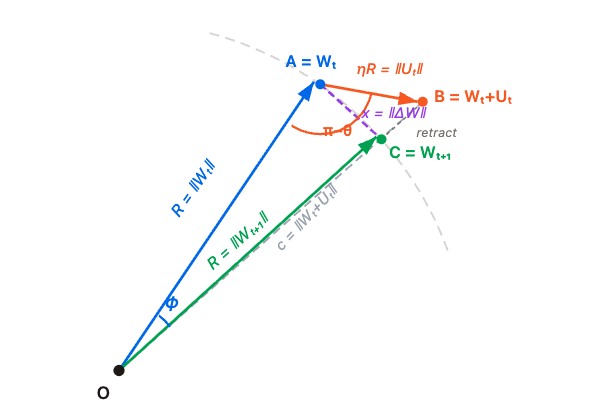
\includegraphics[width=0.75\linewidth]{images/hyperball_cross_section.png}
\caption{Hyperball retraction geometry.}
\label{fig:retraction-geometry}
\end{figure}

The figure shows the 2D cross-section used for the derivation, with the relevant lengths and angles labeled.

We now derive the exact step size. Using the cosine rule on triangle $O$-$A$-$B$ (where $O$ is the origin, $A = W_t$, and $B = W_t + U_t$), noting that the interior angle at $A$ is $\pi - \theta$:

\[
\begin{aligned}
\|W_t+U_t\|^2
&= R^2 + \eta^2 R^2 - 2\eta R^2\cos(\pi-\theta) \\
&= R^2 + \eta^2 R^2 + 2\eta R^2\cos\theta.
\end{aligned}
\]
Hence the pre-retraction length is
$c := \|W_t+U_t\| = R \sqrt{1 + \eta^2+ 2\eta \cos\theta}$.

Since $W_{t+1}$ lies on the ray from $O$ through $B$, the angular change $\phi := \angle(\vec W_t, \vec W_{t+1})$ equals $\angle AOB$. Applying the sine rule to $\triangle OAB$:
\[
\frac{\sin\phi}{\|U_t\|}
  =\frac{\sin(\pi-\theta)}{\|W_t+U_t\|}
  \;\implies\;
\sin\phi
  =\frac{\eta R}{c}\sqrt{1-\gamma^2},
\]
and therefore
\[
\cos\phi
  =\sqrt{1-\sin^2\phi}
  =\sqrt{1-\frac{\eta^2(1-\gamma^2)}{1+\eta^2+2\eta\gamma}}.
\]

Finally, $W_t$ and $W_{t+1}$ both lie on the sphere of radius $R$, so we apply the cosine rule to the isosceles triangle $\triangle OAC$:

\[
\begin{aligned}
\|\Delta W\|^2 &= R^2+R^2-2R^2\cos\phi,\\
x := \|\Delta W\| &= R\sqrt{2}\sqrt{1-\cos\phi}\\
&= R\sqrt{2}\sqrt{1-\sqrt{1-\frac{\eta^2(1-\gamma^2)}{1+\eta^2+2\eta\gamma}}}.
\end{aligned}
\]

This exact expression also recovers the intuitive $O(\eta)$ relative-step-size argument. Hyperball sets both $\|W_t\|=R$ and $\|U_t\|=\eta R$. If $\|\Delta W\|_F$ is on the same order as $\|U_t\|_F$, then
\[
\frac{\|\Delta W\|_F}{\|W_t\|_F}
=\frac{O(\|U_t\|_F)}{\|W_t\|_F}
=O(\eta).
\]
The exact formula above refines this by accounting for the alignment between $W_t$ and $U_t$.

\paragraph{Small-learning-rate regime.} In our practical training regime, $\eta^2\ll 1$ and $\gamma\eta\ll 1$, so $1+\eta^2+2\eta\gamma\approx 1$ and
\[
x\approx R\sqrt{2}\sqrt{1-\sqrt{1-\eta^2(1-\gamma^2)}}.
\]
Applying $\sqrt{1-z}\approx 1-z/2$ yields
\[
x \;\approx\; R\sqrt{2}\sqrt{1-\bigl(1-\tfrac{1}{2}\eta^2(1-\gamma^2)\bigr)}
\;=\; R\,\eta\sqrt{1-\gamma^2}
\;=\; R\,\eta\sin\theta.
\]
Since $\|W_t\|=R$, the relative step size is
\[
\frac{x}{\|W_t\|} \;\approx\; \eta\,\sqrt{1-\gamma^2}.
\]
When the update is orthogonal to the current weights ($\gamma=0$), this collapses to $\frac{x}{\|W_t\|}\approx \eta$. Thus, in this regime, doubling the learning rate approximately doubles the effective movement on the sphere.


\section{Bounds on the Relative Step Size}
\label{app:bounds}

We restrict to $\gamma,\eta\in(0,1)$ throughout this appendix; the $\gamma\in(-1,0)$ case follows by replacing $\gamma\to|\gamma|$ in every step (the formula is dominated by $\gamma^2$, and the linear $2\eta\gamma$ term in the denominator only tightens the bound when $\gamma<0$). Now, suppose we know that $\gamma,\eta\in(0,1)$. We can infer from this that:

\[
\begin{aligned}
\min_{\gamma,\eta\in[0,1]} \frac{\eta^2-\gamma^2\eta^2}{1+\eta^2+2\eta\gamma} = 0
\;&\implies\;
\inf_{\gamma,\eta\in(0,1)} \frac{\eta^2-\gamma^2\eta^2}{1+\eta^2+2\eta\gamma} = 0 \\
\argmax_{\gamma,\eta\in[0,1]} \frac{\eta^2-\gamma^2\eta^2}{1+\eta^2+2\eta\gamma} =
(0,1)\;&\implies\;
\sup_{\gamma,\eta\in(0,1)}\frac{\eta^2-\gamma^2\eta^2}{1+\eta^2+2\eta\gamma}=\tfrac{1}{2}
\end{aligned}
\]
From this we obtain
\[
\begin{aligned}
&\frac{\eta^2-\gamma^2\eta^2}{1+\eta^2+2\eta\gamma}\in (0,\tfrac{1}{2})
\;\implies\;
\sqrt{1-\frac{\eta^2-\gamma^2\eta^2}{1+\eta^2+2\eta\gamma}}\in
(\tfrac{1}{\sqrt2},1)\\
&\implies
1-\sqrt{\cdots}\in
(0,1-\tfrac{1}{\sqrt2})
\;\implies\;
\sqrt{1-\sqrt{\cdots}}\in
(0,\sqrt{1-\tfrac{1}{\sqrt2}})\\
&\implies x\in \bigl(0,\; R\sqrt{2-\sqrt{2}}\bigr)
\approx (0,\; 0.765R)\\
&\implies \frac{x}{\|W_t\|}\in (0,\;\sqrt{2-\sqrt{2}})\approx (0,\; 0.765)
\end{aligned}
\]

This is the tightest bound on the relative step size obtainable without knowledge of $\gamma$. Computing $\gamma$ analytically remains an open question, as the repeated retractions onto the hypersphere make it difficult to translate previous arguments involving momentum and weight decay~\citep{hyperball}. Unfortunately, this bound is not particularly informative: the lower bound is vacuous, and the upper bound is substantially looser than the ideal $O(\eta)$. Now, if, for instance, we input our tried and tested range $\sim\eta\in (10^{-4},10^{-1})$ and fix $\gamma=0$, we get a slightly tighter bound of $(0.0001, 0.0996)$, where a higher learning rate corresponds to a higher step size. For a higher dot product like $\gamma=0.5$, we get a bound of $(0.0000866, 0.0823)$, which is lower.


\section{Enforcing Scale Invariance}
\label{app:scale-inv}

A key ingredient is RMSNorm~\citep{rmsnorm}, which rescales a vector by its root-mean-square (RMS) magnitude. Given an activation vector $x\in\mathbb{R}^d$, RMSNorm computes
\[
\mathrm{RMSNorm}(x) = g\odot \frac{x}{\sqrt{\frac{1}{d}\sum_{i=1}^d x_i^2 + \varepsilon}},
\]
where $g\in\mathbb{R}^d$ is a learned per-coordinate gain, $\varepsilon>0$ is for numerical stability, and $\odot$ is the Hadamard product (element-wise multiplication).

\paragraph{Rescaling property.}
Ignoring $\varepsilon$ (or when $\|x\|$ is not tiny), RMSNorm is \emph{scale invariant}: for any scalar $\alpha>0$,
\[
\mathrm{RMSNorm}(\alpha x)= \mathrm{RMSNorm}(x).
\]
Intuitively, scaling the input by $\alpha$ scales the denominator by the same $\alpha$, so the normalized direction stays the same.

\paragraph{Why this makes weight matrices scale invariant.}
Consider a linear map $y = Wx$. If the model applies RMSNorm before the next computation (pre-norm, post-norm, or both), then multiplying the weight matrix by a scalar often has little effect on the downstream activations:
\[
\mathrm{RMSNorm}((\alpha W)x) = \mathrm{RMSNorm}(\alpha (Wx)) = \mathrm{RMSNorm}(Wx).
\]
So for these ``RMSNorm sandwiched'' layers, scale doesn't matter as the RMSNorm layer itself learns the scaling factor necessary for the output.

In our model architecture, we used MuP initialization and layer pre-normalization, but that was not enough to enforce scale invariance. To further enforce it, we added a layer post-norm and then QK-norm (like Gemma~3's and ~4's architecture~\citep{gemma}), which appeared to be sufficient for our model (although adding only the post-norm may already have been enough; the QK-norm was added for completeness).


\section{Why Gradient Statistics Differ}
\label{app:gradient-stats}

Consider a vocabulary of $K$ tokens with marginal frequencies $p_1\ge p_2\ge\cdots\ge p_K$. In a mini-batch of $B$ tokens drawn i.i.d.\ from $p$, the expected count of token $k$ is $n_k=B\,p_k$. The gradient of the loss decomposes as
\[
g = \frac{1}{B}\sum_{k=1}^{K} n_k\,\bar g_k
  = \sum_{k=1}^{K} p_k\,\bar g_k,
\]
where $\bar g_k$ is the mean gradient contribution conditioned on token $k$. We can say that Adam's running second moment for parameters associated with token $k$ accumulates as $v_k\propto p_k\,\mathbb{E}[\|\bar g_k\|^2]+(1-p_k)\,\bar 0=p_k\,\mathbb{E}[\|\bar g_k\|^2]$. The ratio of the largest to smallest second moment therefore scales with the frequency ratio of the most to least common token
$\frac{v_1}{v_K}\;\propto\;\frac{p_1\,\mathbb{E}[\|\bar g_1\|^2]}{p_K\,\mathbb{E}[\|\bar g_K\|^2]}$.
If we assume that $\frac{\mathbb{E}[\|\bar g_1\|^2]}{\mathbb{E}[\|\bar g_K\|^2]}\approx O(1)$, then:
\[
\frac{v_1}{v_K}\;\propto\;\frac{p_1}{p_K}
\]

\textbf{Zipf (NLP):} With $p_k\propto 1/k$ and $K\approx 100{,}000$, the dynamic range is $p_1/p_K\approx K\approx 10^5$. Adam's per-coordinate $1/\sqrt{v_k}$ scaling spans \emph{orders of magnitude}, providing substantial per-direction adaptation that compensates for the wildly uneven gradient contributions of frequent vs.\ rare tokens.

\textbf{DNA:} With $K=4$ and $p_k\approx 1/4$, the dynamic range is $p_1/p_K\approx 1$. Adam's adaptive denominator $\sqrt{v_k}$ is nearly identical across all tokens, reducing the coordinate-wise scaling to an approximately uniform scalar. The per-direction adaptation that makes Adam powerful in NLP provides \emph{negligible benefit} here, while Muon's whitened, scale-free updates are naturally suited to this near-isotropic landscape.


\section{Why Does Hyperball Worsen Muon?}
\label{app:hyperball-worsen}

We hypothesize that this is because Hyperball's re-projection scales all singular values of the weight matrix by the \emph{same} multiplicative factor. When Hyperball maps $W_{t+1} = R\,(W_t + U_t)/\|W_t + U_t\|_F$, it shrinks every singular direction of $W$ equally\footnote{It is actually possible to be on both the Frobenius and Spectral sphere at once as they DO intersect, but our algorithm does not guarantee that we enter the intersection. As a clarification: There exists an inequality $\|W\|_2\le \|W\|_F\le \sqrt{\min(m, n)}\|W\|_2$, so one might believe that $\|W\|_F\in[1,\sqrt{\min(m, n)}]$ guarantees that $W$ lies in the intersection, but this is a necessary condition, not a sufficient one (think of a rank 1 matrix within this range)!}. The dominant singular values of $W$, being large, survive this downscaling, and they remain the dominant share of the fixed energy budget $\|W\|_F^2 = \sum_i \sigma_i^2 = R^2$. The smaller singular values of $W$, however, cannot: Muon's whitening of the update matrix tries to grow them step after step by distributing the learning signal equally across all singular directions, but the uniform rescaling of the weight matrix pulls them back down proportionally each time. Because they never accumulate enough energy to matter, the small directions effectively die while the large ones persist, concentrating the spectrum into fewer and fewer dominant modes. The spectral metrics in Section~\ref{sec:spectral} support this: MuonH's spectral entropy and participation ratio collapse over training, consistent with the small singular directions being progressively eroded by the uniform rescaling.

Adam under the same Hyperball constraint does not suffer this fate, because without whitening the spectrum is already concentrated in the task-relevant directions; the uniform rescaling therefore does comparatively little damage. Weight decay, on the other hand, does \emph{not} alter the Muon update at all, it only decays the matrix the update is added to, so the whitening and the regularizer rarely conflict.


\section{Why Isn't Muon's Update Full-Rank?}
\label{app:delta-w-rank}

One might expect Muon's whitening step to produce a perfectly uniform spectrum, but in practice the Newton--Schulz iterations used to approximate the polar factor are finite (typically 5 iterations), pushing singular values only \emph{toward} 1 rather than exactly to 1 (roughly into $[0.7, 1.3]$). More importantly, if the underlying momentum matrix has near-zero singular values, finite iterations cannot lift those values appreciably. Additionally, our Nesterov momentum means NS${}_5$ whitens a lookahead lerp of the gradient and the momentum buffer, not the gradient at $W_t$ itself, so the spectral structure of $U_t$ already reflects a blended signal. Finally, note that $\Delta W \neq U_t$: with independent weight decay, $\Delta W = W_{t+1} - W_t = U_t - \lambda W_t$, so the actual weight change includes a decay term $-\lambda W_t$ whose spectral structure is that of the current weights, not the whitened update.


\section{Note on Adam's Spectral Entropy}
\label{app:note-adam}

AdamW (Orange) maintains high entropy (relative to AdamH and MuonH), potentially because coordinate-wise updates can sustain activity in smaller singular directions by injecting noise. MuonW achieves high entropy through `clean' whitened updates that amplify rare directions. This distinction aligns with NerVE's~\citep{nerve} finding that stable spectral signatures correlate with generalization ability and respond predictably to optimizer design choices.


\section{FLOPs Accounting}
\label{app:flops}

Each FLOPs-axis plot uses a per-optimizer cost model that accounts for both the per-token forward/backward compute and the per-step optimizer update. Let
\begin{itemize}
  \item $L$: sequence length (tokens per sequence),
  \item $B$: batch size (sequences per step),
  \item $N$: total sequences in the dataset,
  \item $P_{\text{2D}}$: total 2D parameters (linear weights and embeddings); optimized by Muon/MuonH in mixed mode and dominating forward/backward matmul compute,
  \item $P_{\text{non-2D}}$: total non-2D parameters (RMSNorm scales, any biases); under the mixed-Muon optimizers (MuonW and MuonH) these are handled by an AdamW sub-optimizer, while under plain AdamW or AdamH all parameters share the top-level optimizer,
  \item $d$: hidden dimension,
  \item $C_{\text{opt}}$: per-parameter FLOP cost of a single optimizer step.
\end{itemize}

Total FLOPs for one epoch decompose into a \emph{base compute} term (forward/backward, incurred once per token) and an \emph{optimizer overhead} term (incurred once per batch step). We use the standard $6\,P_{\text{2D}}$-FLOPs-per-token matmul proxy for the base compute, which ignores non-matmul ops (attention softmax/mask, activations, norms, embedding lookups) contributing a few percent at $L = 352$, $d = 2048$:
\begin{align*}
\text{Base compute} &\approx 6\,P_{\text{2D}}\,(N\,L), \\
\text{Optimizer overhead} &\approx \bigl(P_{\text{2D}}\,C_{\text{opt}}^{\text{Muon}} + P_{\text{non-2D}}\,C_{\text{opt}}^{\text{AdamW}}\bigr)\,(N/B).
\end{align*}
In our architecture $P_{\text{non-2D}} \ll P_{\text{2D}}$ (under $1\%$ of total parameters), so we drop the non-2D overhead contribution and factor $P_{\text{2D}}\,N$ out of the master formula. For brevity we write $P$ for $P_{\text{2D}}$ for the remainder of this appendix:
\[
F(L, B, N) \;\approx\; P\,N\!\left(6L + \frac{C_{\text{opt}}}{B}\right).
\]

\paragraph{Per-optimizer step costs.} Applying this to our four optimizers (with $C_{\text{opt}}$ derived by counting scalar FLOPs per parameter for each kernel in the \texttt{step()} method of the PyTorch implementation, under our fused SwiGLU architecture):
\begin{align*}
\text{AdamW}\quad & C_{\text{opt}} = \underbrace{3}_{m_1} + \underbrace{4}_{m_2} + \underbrace{3}_{\text{denom}} + \underbrace{1}_{\lambda} + \underbrace{3}_{\text{step}} = 14, \\
\text{AdamH}\quad & C_{\text{opt}} = \underbrace{3}_{m_1} + \underbrace{4}_{m_2} + \underbrace{3}_{\text{denom}} + \underbrace{2}_{\hat m_1} + \underbrace{8}_{\text{HB}} = 20, \\
\text{MuonW}\quad & C_{\text{opt}} = \underbrace{6}_{\text{lerps}} + \underbrace{3}_{\text{spec-norm}} + \underbrace{23.125\,d + \tfrac{445}{28}}_{\text{5 NS}} + \underbrace{3}_{\text{step}} \;=\; 23.125\,d + \tfrac{781}{28} \;\approx\; 23.125\,d + 27.89, \\
\text{MuonH}\quad & C_{\text{opt}} = \underbrace{6}_{\text{lerps}} + \underbrace{3}_{\text{spec-norm}} + \underbrace{23.125\,d + \tfrac{445}{28}}_{\text{5 NS}} + \underbrace{8}_{\text{HB}} \;=\; 23.125\,d + \tfrac{921}{28} \;\approx\; 23.125\,d + 32.89.
\end{align*}
Each component counts the per-parameter FLOPs of one PyTorch kernel in the step (under the conventions $a\mathbin{{+}{=}}\alpha b$ = 2 FLOPs/elt, \texttt{addcmul\_} and \texttt{addcdiv\_} = 3 FLOPs/elt, and $\|\cdot\|_F$ = 2 FLOPs/elt). For Adam, $m_1$ is the first-moment EMA ($\texttt{mul\_}+$axpy), $m_2$ is the second-moment EMA ($\texttt{mul\_}+\texttt{addcmul\_}$), and ``denom'' is $(\sqrt{\hat v_t}/\sqrt{b_2})+\varepsilon$; the AdamW tail is a decoupled weight-decay scale $\lambda$ plus a fused \texttt{addcdiv\_} ``step'' ($1+3$), whereas AdamH replaces it with a bias-correction divide $\hat m_1$ ($\texttt{exp\_avg}/b_1$, 2) and an 8-FLOP \emph{Hyperball} (HB) projection $\{\,u\leftarrow m/\text{denom},\ \|u\|_F,\ u\!\cdot\!R/\|u\|_F,\ p\mathrel{{+}{=}}\!-\eta u,\ \|p\|_F,\ p\!\cdot\!R/\|p\|_F\,\}$. For Muon, the 6-FLOP ``lerps'' are the in-place momentum-buffer update \texttt{buf.lerp\_(grad,\ 1-m)} and the out-of-place Nesterov lookahead \texttt{update\ =\ grad.lerp(buf,\ m)} (3 FLOPs each: one \texttt{mul\_} plus one axpy); the 3-FLOP ``spec-norm'' is the Frobenius pre-divide $\tilde U\leftarrow U/\|U\|_F$ that feeds Newton--Schulz; the MuonW/MuonH tails are identical to the AdamW/AdamH tails above (``step'' = weight decay + scaled add, $1+2=3$; ``HB'' = same 8-FLOP projection).

\paragraph{Deriving the Muon Newton--Schulz cost.} The $d$-dependent $23.125\,d + \tfrac{445}{28}$ term sums the five Newton--Schulz iterations across all Muon-eligible weights in one transformer layer. Each iteration performs three matrix ops on a single weight of shape $[m, n]$ with $m \le n$ (the code transposes if $m > n$): a Gram product $G \leftarrow \tilde U \tilde U^\top$ ($2 m^2 n$ matmul FLOPs), a cubic \texttt{addmm} $G \leftarrow b G + c G^2$ ($2 m^3 + 3 m^2$), and a final \texttt{addmm} $\tilde U \leftarrow a \tilde U + G \tilde U$ ($2 m^2 n + 2 m n$). Per parameter, 5 iterations cost $20 m + 10\,m^2/n$ matmul FLOPs and $10 + 15\,m/n$ scaling FLOPs, so the cost depends on each weight's post-transpose aspect ratio $r = m/n$. Summing over the six per-layer Muon-eligible weights of a grouped-query-attention ($g \equiv \text{num\_kv\_groups}/\text{num\_heads} = 2/8 = 1/4$) + SwiGLU block with $d_{\text{ff}} = 8 d/3$:

\begin{center}
\begin{tabular}{l c c r r r}
\toprule
Weight & $[m, n]$ & $r$ & Params & 5-step matmul & 5-step scaling \\
\midrule
$W_q, \texttt{out\_proj}$ (each) & $[d, d]$ & $1$ & $d^2$ & $30\,d^3$ & $25\,d^2$ \\
$W_k, W_v$ (each) & $[d/4, d]$ & $1/4$ & $d^2/4$ & $45\,d^3/32$ & $55\,d^2/16$ \\
\texttt{up\_proj} & $[d, 16d/3]$ & $3/16$ & $16\,d^2/3$ & $350\,d^3/3$ & $205\,d^2/3$ \\
\texttt{down\_proj} & $[d, 8d/3]$ & $3/8$ & $8\,d^2/3$ & $190\,d^3/3$ & $125\,d^2/3$ \\
\midrule
\textbf{Per-layer total} & & & $10.5\,d^2$ & $242.8125\,d^3$ & $166.875\,d^2$ \\
\textbf{Per parameter} & & & & $23.125\,d$ & $\tfrac{445}{28} \approx 15.89$ \\
\bottomrule
\end{tabular}
\end{center}

These per-parameter averages are \emph{exact} under the combination of grouped-query attention with $g = 1/4$ and $d_{\text{ff}} = 8 d / 3$ SwiGLU. For a uniformly-square set of weights the cost would be the cleaner $30 d + 25$; the $[d/4, d]$ shape of $W_k, W_v$ and the $8/3$ MLP expansion both pull the matmul coefficient down from $30 d$ to $23.125\,d$ and the constant from $25$ to $445/28$.

For our concrete architecture ($d = 2048$), MuonW's and MuonH's step costs evaluate to $47{,}387.89$ and $47{,}392.89$ FLOPs per parameter, respectively.

\paragraph{Checkpoint-to-FLOPs conversion.} The FLOPs axis in Figures~\ref{fig:perp-by-lr-1}--\ref{fig:perp-by-optimizer-muon} maps a checkpoint index $t$ (a training step) to cumulative FLOPs via
\[
\mathrm{FLOPs}(t, \text{opt}) \;=\; t\,P\!\left(6BL + C_{\text{opt}}^{\text{opt}}\right).
\]

\paragraph{Overhead ratio.} The fraction of compute consumed by the optimizer step relative to the base forward/backward pass is
\[
\frac{C_{\text{opt}}/B}{6L} \;=\; \frac{C_{\text{opt}}}{6\,B\,L},
\]
which is independent of the dataset size $N$. For our largest configuration ($L = 352$, $B = 1920$, $d = 2048$), MuonH's $C_{\text{opt}} \approx 47{,}392.89$ yields an overhead of roughly $1.17\%$, confirming that Muon's Newton--Schulz orthogonalization step is a small fraction of total training FLOPs despite its $O(d)$ scaling in $C_{\text{opt}}$.


% ============================================================
\section{Additional Figures}
\label{app:figures}
% ============================================================

\begin{figure}[htbp]
  \centering
  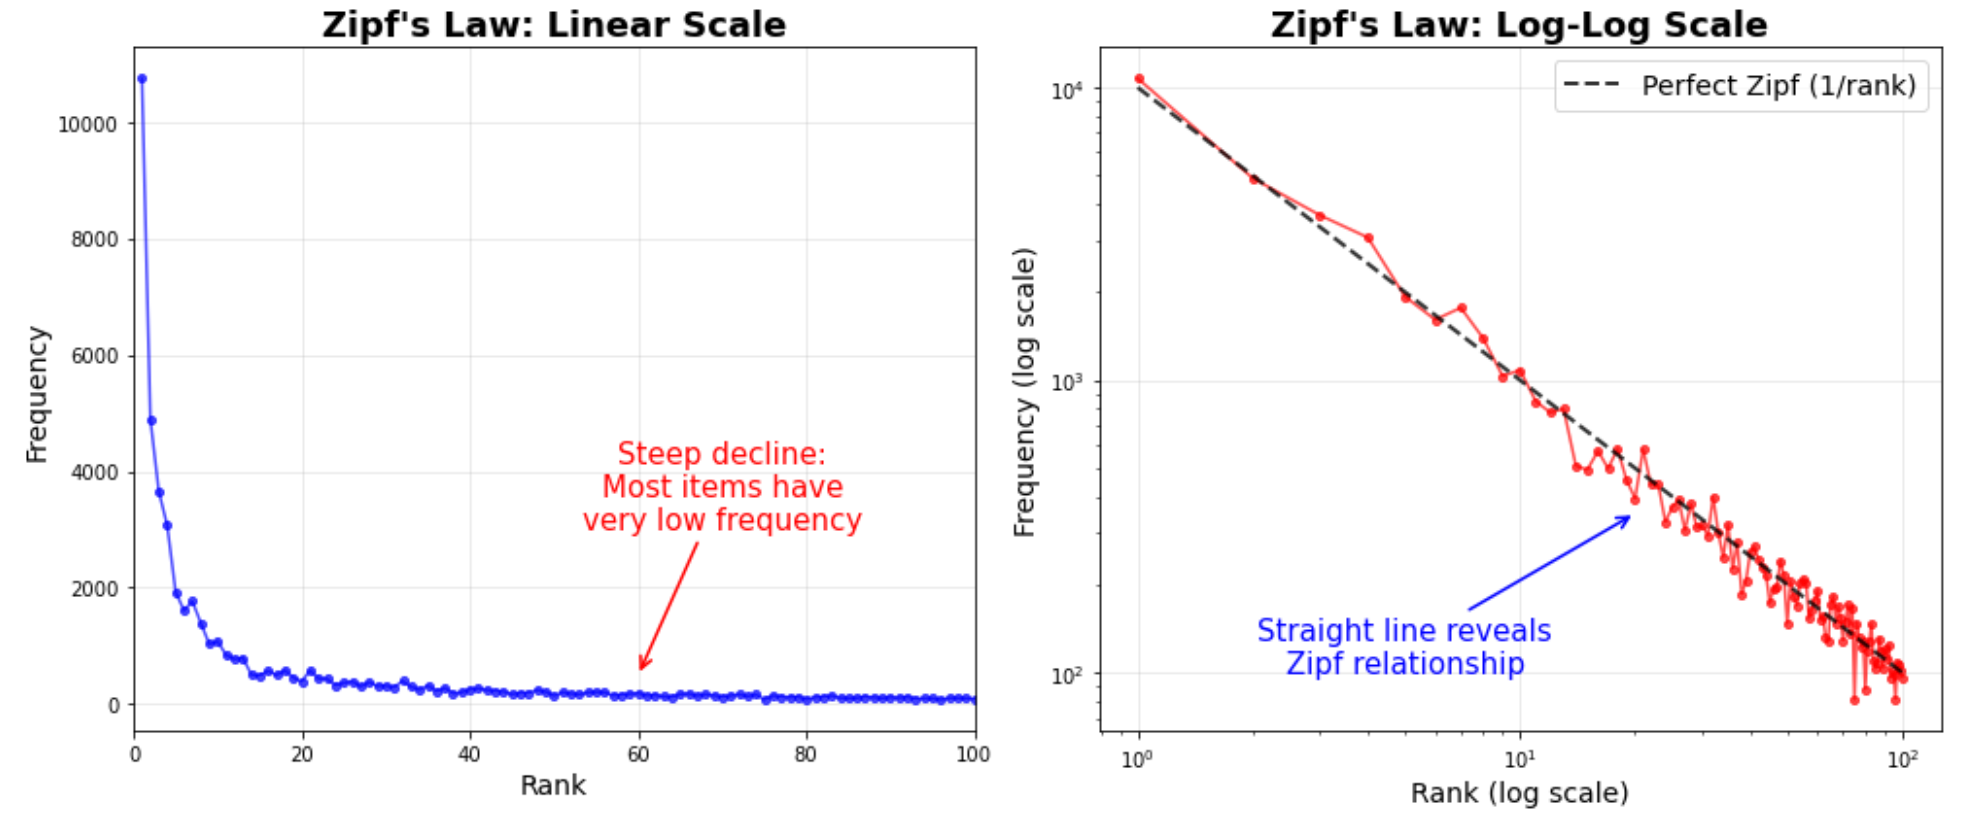
\includegraphics[width=0.85\linewidth]{images/zipfs_law.png}
  \caption{Zipf's law.}
  \label{fig:zipf}
\end{figure}

The left panel shows Zipf's law on a linear scale, and the right panel shows it on a log-log scale. The straight line on the log-log plot is the signature of a power-law distribution. Source: Statology~\citep{zipf}.

\begin{figure}[htbp]
  \centering
  \begin{subfigure}[t]{0.3\linewidth}
    \centering
    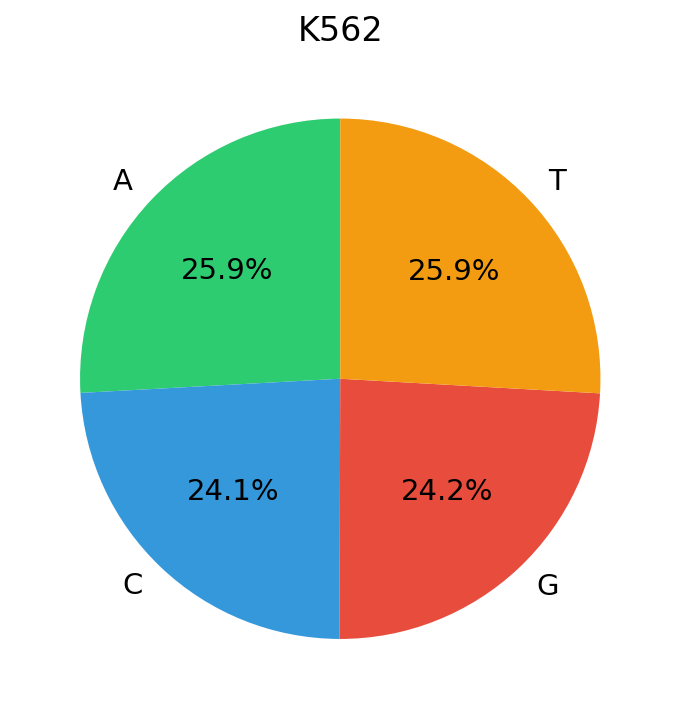
\includegraphics[width=\linewidth]{images/nucleotide_K562_pie.png}
  \end{subfigure}\hfill
  \begin{subfigure}[t]{0.3\linewidth}
    \centering
    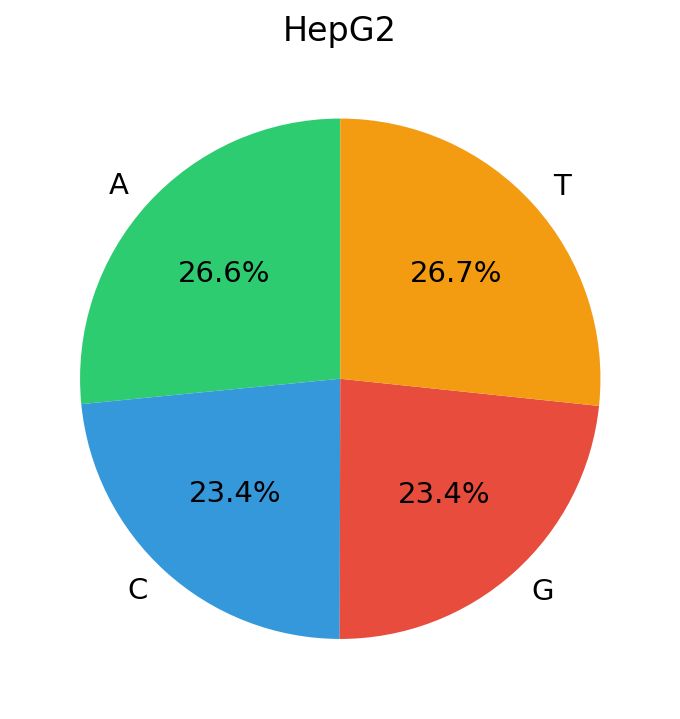
\includegraphics[width=\linewidth]{images/nucleotide_HepG2_pie.png}
  \end{subfigure}\hfill
  \begin{subfigure}[t]{0.3\linewidth}
    \centering
    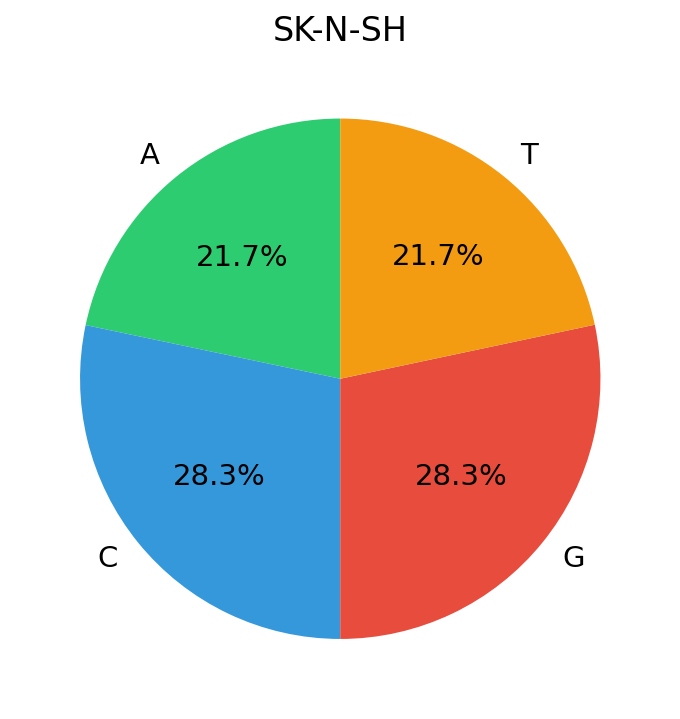
\includegraphics[width=\linewidth]{images/nucleotide_SKNSH_pie.png}
  \end{subfigure}
  \caption{Nucleotide frequencies.}
  \label{fig:nucleotide-dist}
\end{figure}

The panels show nucleotide frequencies across the three cell lines in our training set.

\begin{figure}[htbp]
  \centering
  \begin{subfigure}[t]{0.48\linewidth}
    \centering
    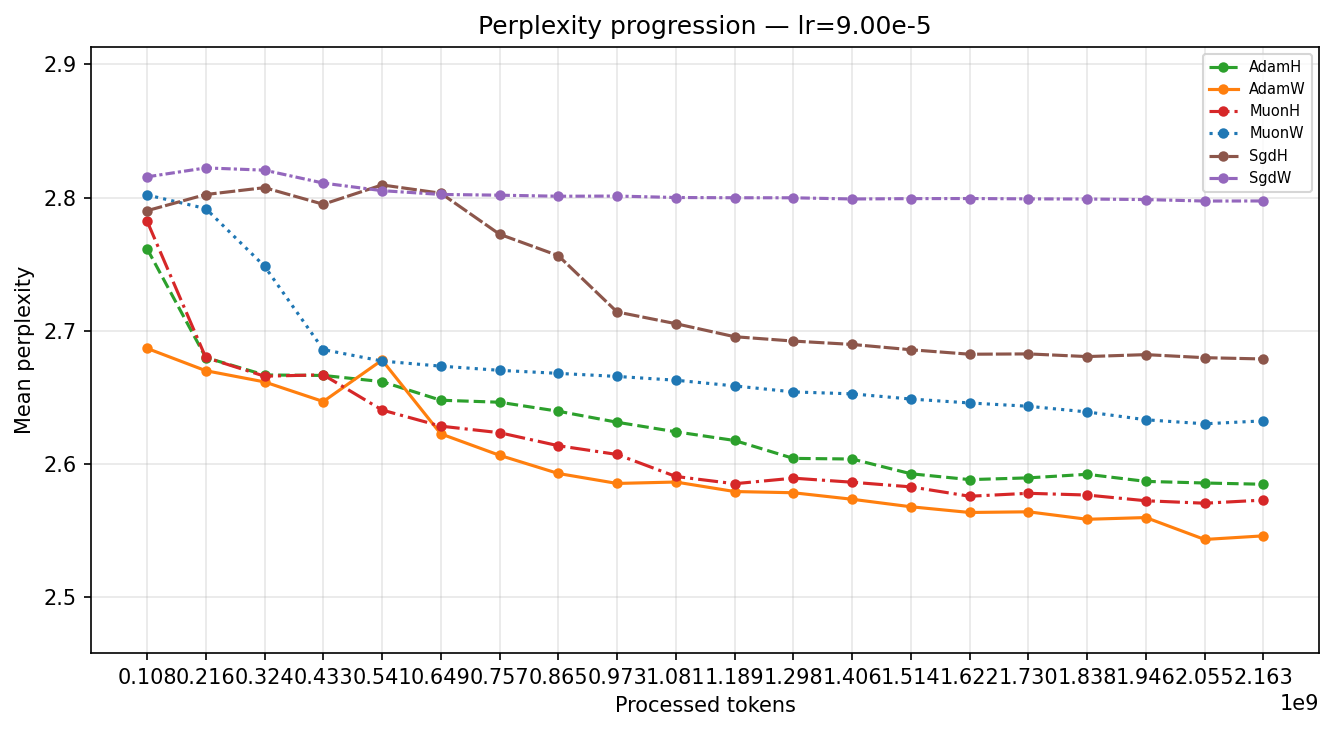
\includegraphics[width=\linewidth]{images/perplexity_progression_lr_9em05.png}
    \caption*{By checkpoint}
  \end{subfigure}\hfill
  \begin{subfigure}[t]{0.48\linewidth}
    \centering
    
\includegraphics[width=\linewidth]{images/perplexity_progression_lr_9em05_flops.png}
    \caption*{By FLOPs}
  \end{subfigure}
  \\[2pt]
  {\small lr $\approx 9.00\times10^{-5}$}

  \medskip
  \begin{subfigure}[t]{0.48\linewidth}
    \centering
    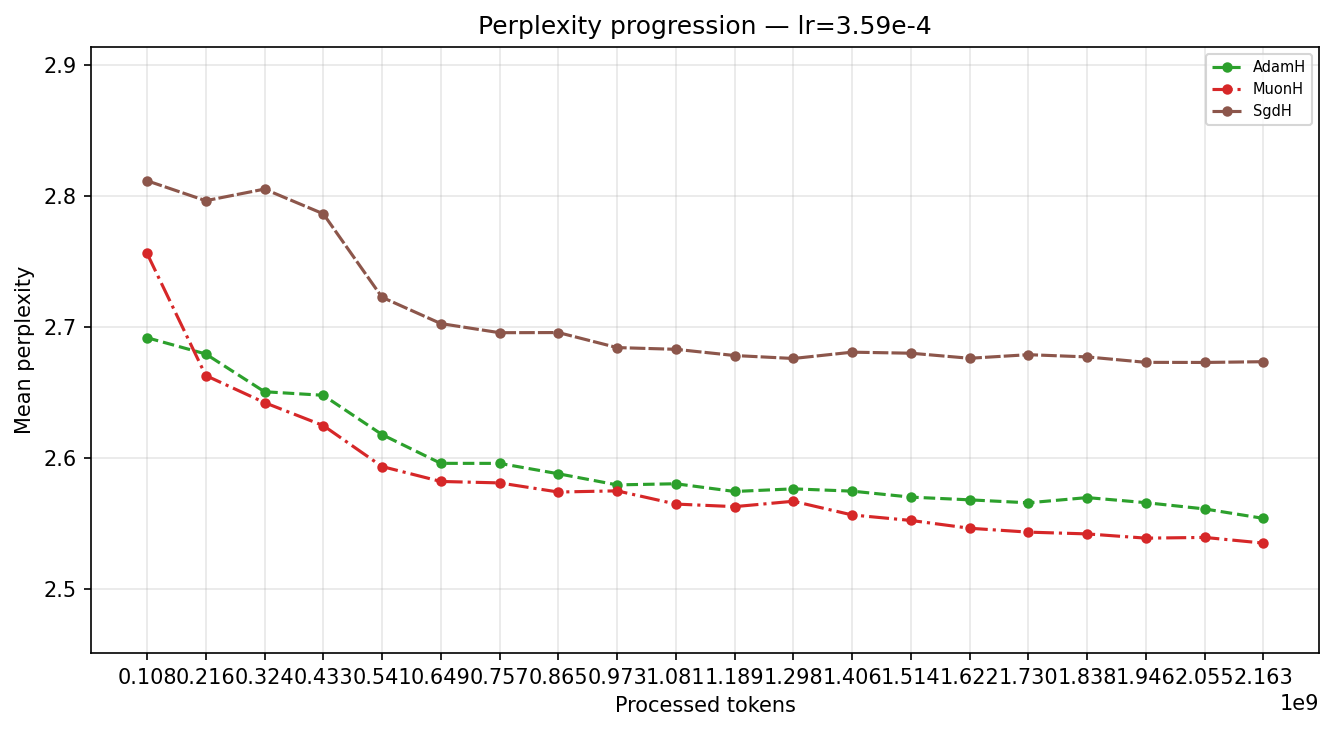
\includegraphics[width=\linewidth]{images/perplexity_progression_lr_0p00035857.png}
  \end{subfigure}\hfill
  \begin{subfigure}[t]{0.48\linewidth}
    \centering
    
\includegraphics[width=\linewidth]{images/perplexity_progression_lr_0p00035857_flops.png}
  \end{subfigure}
  \\[2pt]
  {\small lr $\approx 3.59\times10^{-4}$}

  \medskip
  \begin{subfigure}[t]{0.48\linewidth}
    \centering
    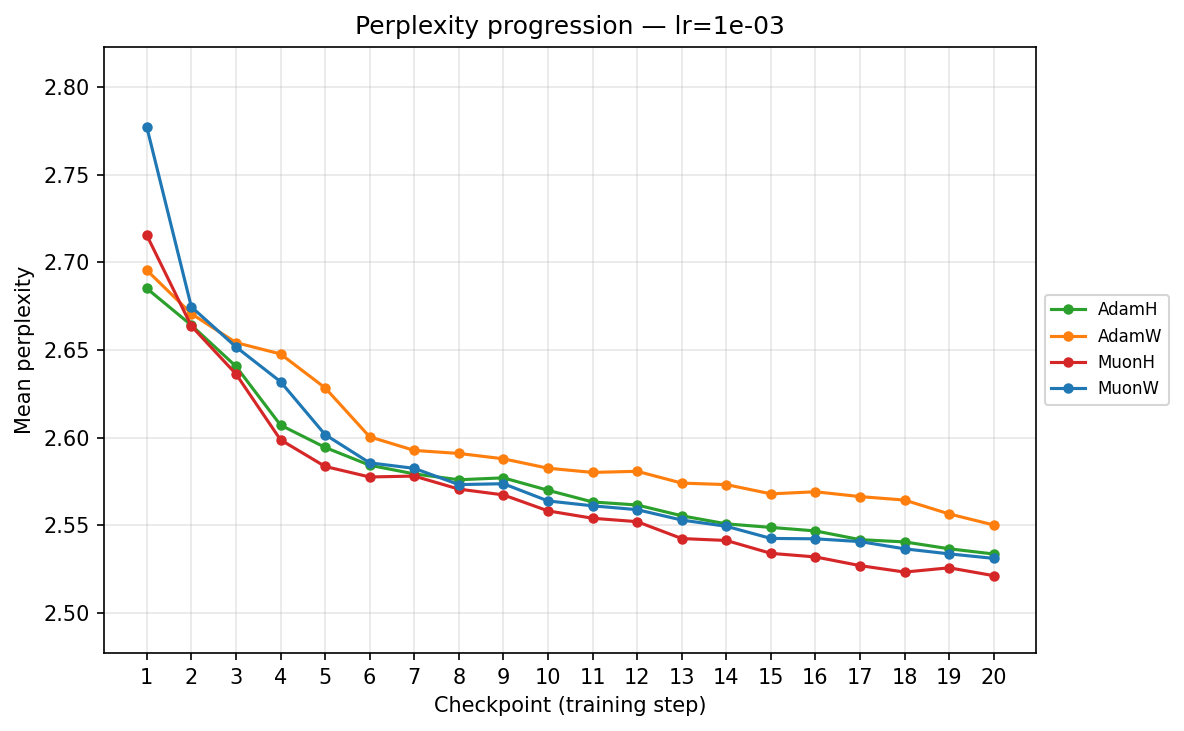
\includegraphics[width=\linewidth]{images/perplexity_progression_lr_0p0014287.png}
  \end{subfigure}\hfill
  \begin{subfigure}[t]{0.48\linewidth}
    \centering
    
\includegraphics[width=\linewidth]{images/perplexity_progression_lr_0p0014287_flops.png}
  \end{subfigure}
  \\[2pt]
  {\small lr $\approx 1.43\times10^{-3}$}

  \caption{Learning-rate sweep perplexity, part 1.}
  \label{fig:perp-by-lr-1}
\end{figure}

The left panels show mean test perplexity over training checkpoints, while the right panels show mean test perplexity over cumulative FLOPs. Lower is better; the FLOP accounting follows the conversion defined above.

\begin{figure}[htbp]
  \centering
  \begin{subfigure}[t]{0.48\linewidth}
    \centering
    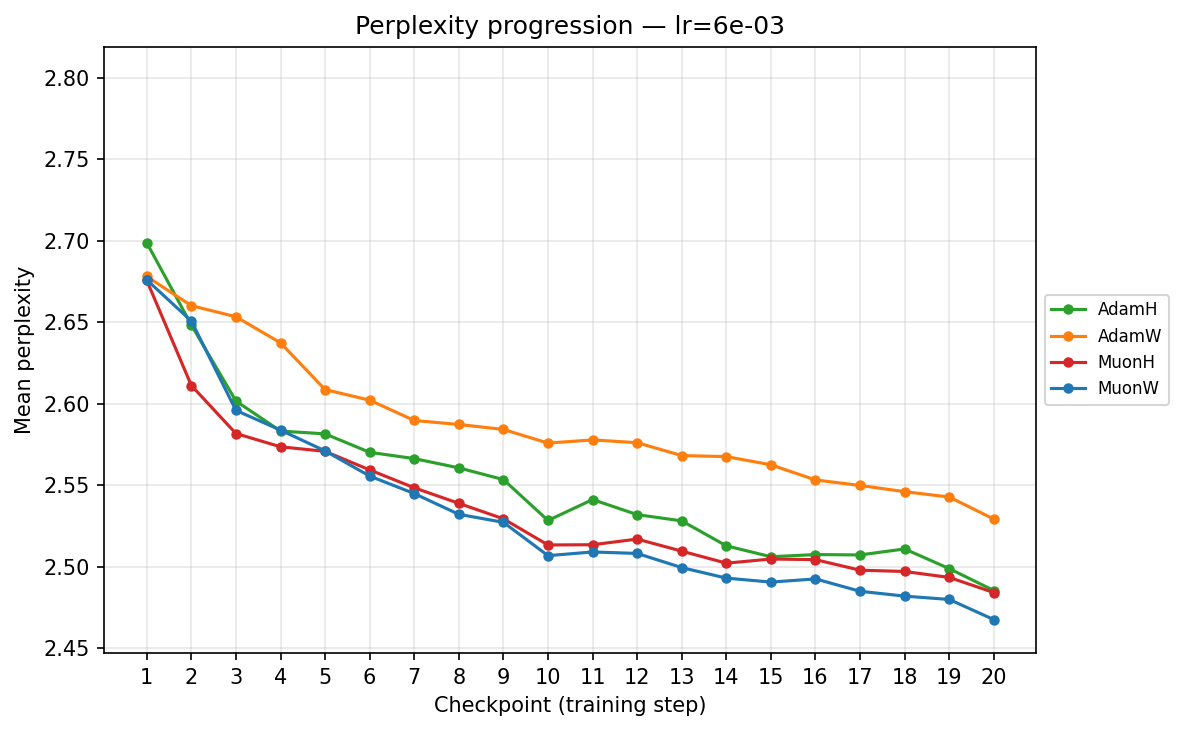
\includegraphics[width=\linewidth]{images/perplexity_progression_lr_0p0056924.png}
    \caption*{By checkpoint}
  \end{subfigure}\hfill
  \begin{subfigure}[t]{0.48\linewidth}
    \centering
    
\includegraphics[width=\linewidth]{images/perplexity_progression_lr_0p0056924_flops.png}
    \caption*{By FLOPs}
  \end{subfigure}
  \\[2pt]
  {\small lr $\approx 5.69\times10^{-3}$}

  \medskip
  \begin{subfigure}[t]{0.48\linewidth}
    \centering
    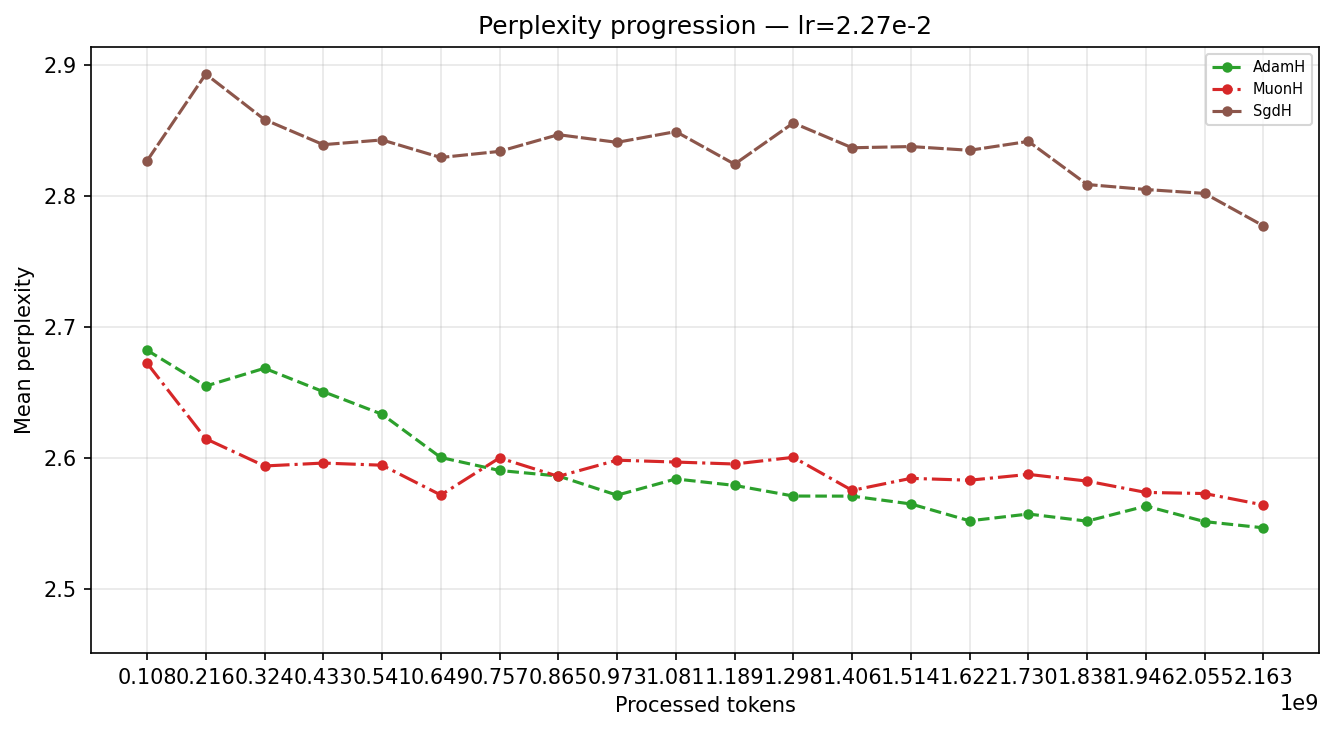
\includegraphics[width=\linewidth]{images/perplexity_progression_lr_0p022681.png}
  \end{subfigure}\hfill
  \begin{subfigure}[t]{0.48\linewidth}
    \centering
    
\includegraphics[width=\linewidth]{images/perplexity_progression_lr_0p022681_flops.png}
  \end{subfigure}
  \\[2pt]
  {\small lr $\approx 2.27\times10^{-2}$}

  \caption{Learning-rate sweep perplexity, part 2.}
  \label{fig:perp-by-lr-2}
\end{figure}

The left panels show mean test perplexity over training checkpoints, while the right panels show mean test perplexity over cumulative FLOPs. Lower is better; the FLOP accounting follows the conversion defined above.

\begin{figure}[htbp]
  \centering
  \begin{subfigure}[t]{0.48\linewidth}
    \centering
    
\includegraphics[width=\linewidth]{images/perplexity_progression_AdamH.png}
    \caption*{By checkpoint}
  \end{subfigure}\hfill
  \begin{subfigure}[t]{0.48\linewidth}
    \centering
    
\includegraphics[width=\linewidth]{images/perplexity_progression_AdamH_flops.png}
    \caption*{By FLOPs}
  \end{subfigure}
  \\[2pt]
  {\small AdamH}

  \medskip
  \begin{subfigure}[t]{0.48\linewidth}
    \centering
    
\includegraphics[width=\linewidth]{images/perplexity_progression_AdamW.png}
  \end{subfigure}\hfill
  \begin{subfigure}[t]{0.48\linewidth}
    \centering
    
\includegraphics[width=\linewidth]{images/perplexity_progression_AdamW_flops.png}
  \end{subfigure}
  \\[2pt]
  {\small AdamW}

  \caption{Adam variant perplexity.}
  \label{fig:perp-by-optimizer-adam}
\end{figure}

The left panels show mean test perplexity over checkpoints, while the right panels show mean test perplexity over cumulative FLOPs. The plots cover five learning rates, using the FLOP conversion defined above.

\begin{figure}[htbp]
  \centering
  \begin{subfigure}[t]{0.48\linewidth}
    \centering
    
\includegraphics[width=\linewidth]{images/perplexity_progression_MuonH.png}
    \caption*{By checkpoint}
  \end{subfigure}\hfill
  \begin{subfigure}[t]{0.48\linewidth}
    \centering
    
\includegraphics[width=\linewidth]{images/perplexity_progression_MuonH_flops.png}
    \caption*{By FLOPs}
  \end{subfigure}
  \\[2pt]
  {\small MuonH}

  \medskip
  \begin{subfigure}[t]{0.48\linewidth}
    \centering
    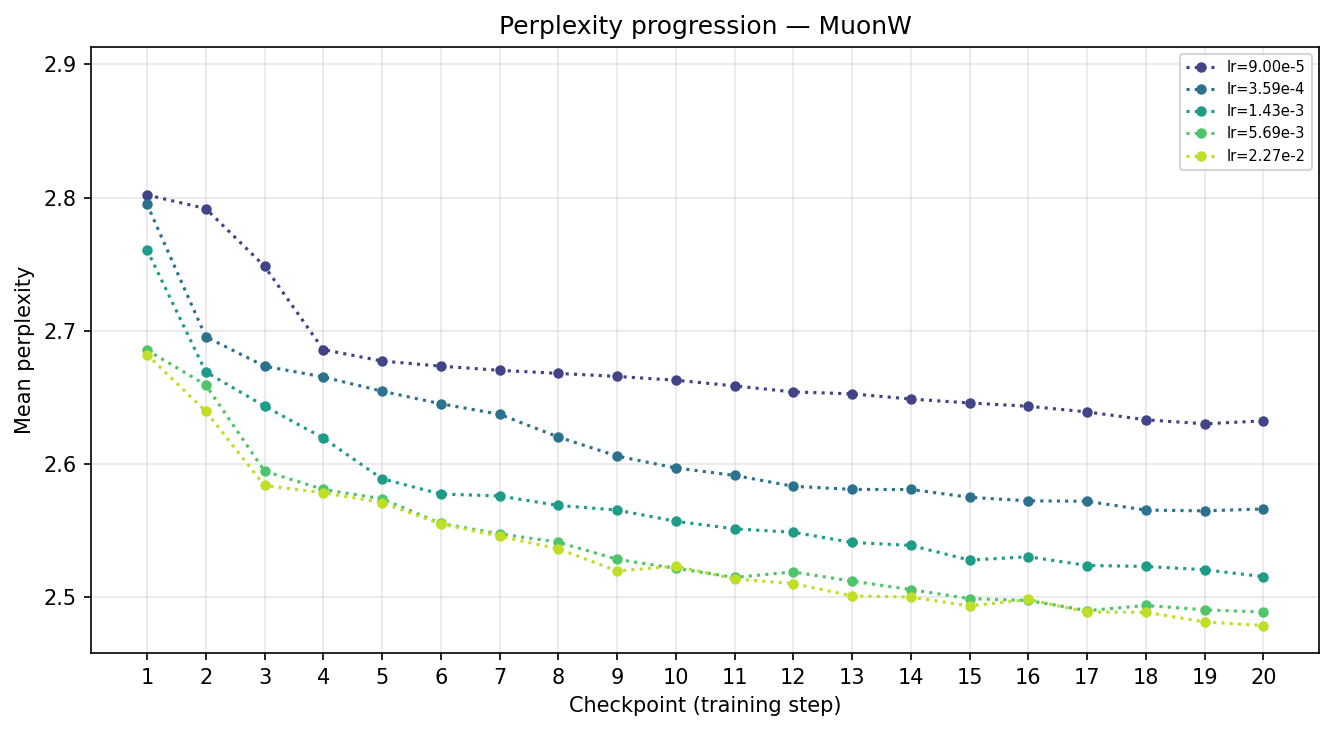
\includegraphics[width=\linewidth]{images/perplexity_progression_MuonW.png}
  \end{subfigure}\hfill
  \begin{subfigure}[t]{0.48\linewidth}
    \centering
    
\includegraphics[width=\linewidth]{images/perplexity_progression_MuonW_flops.png}
  \end{subfigure}
  \\[2pt]
  {\small MuonW}

  \caption{Muon variant perplexity.}
  \label{fig:perp-by-optimizer-muon}
\end{figure}

The left panels show mean test perplexity over checkpoints, while the right panels show mean test perplexity over cumulative FLOPs. The plots cover five learning rates, using the FLOP conversion defined above.

\begin{figure}[htbp]
  \centering
  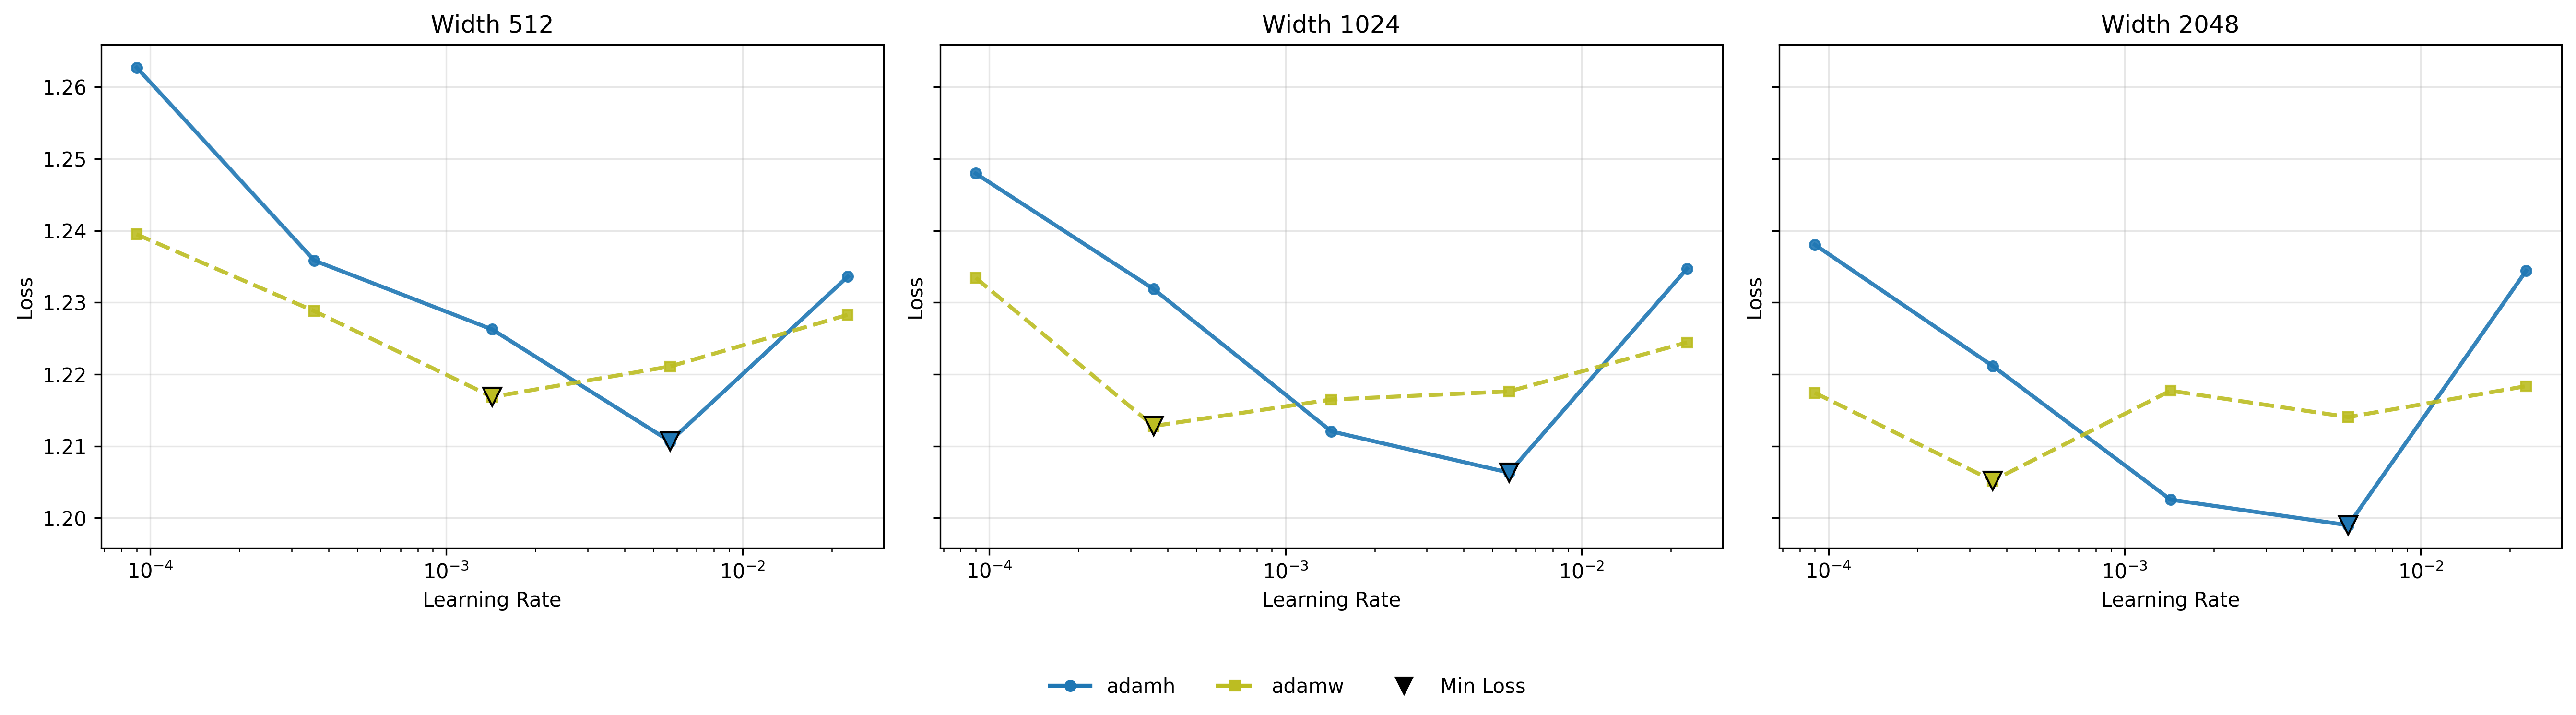
\includegraphics[width=0.85\linewidth]{images/adam_comparison.png}
  \caption{Sweep losses: AdamW vs AdamH.}
  \label{fig:sweep-losses-adam}
\end{figure}

\begin{figure}[htbp]
  \centering
  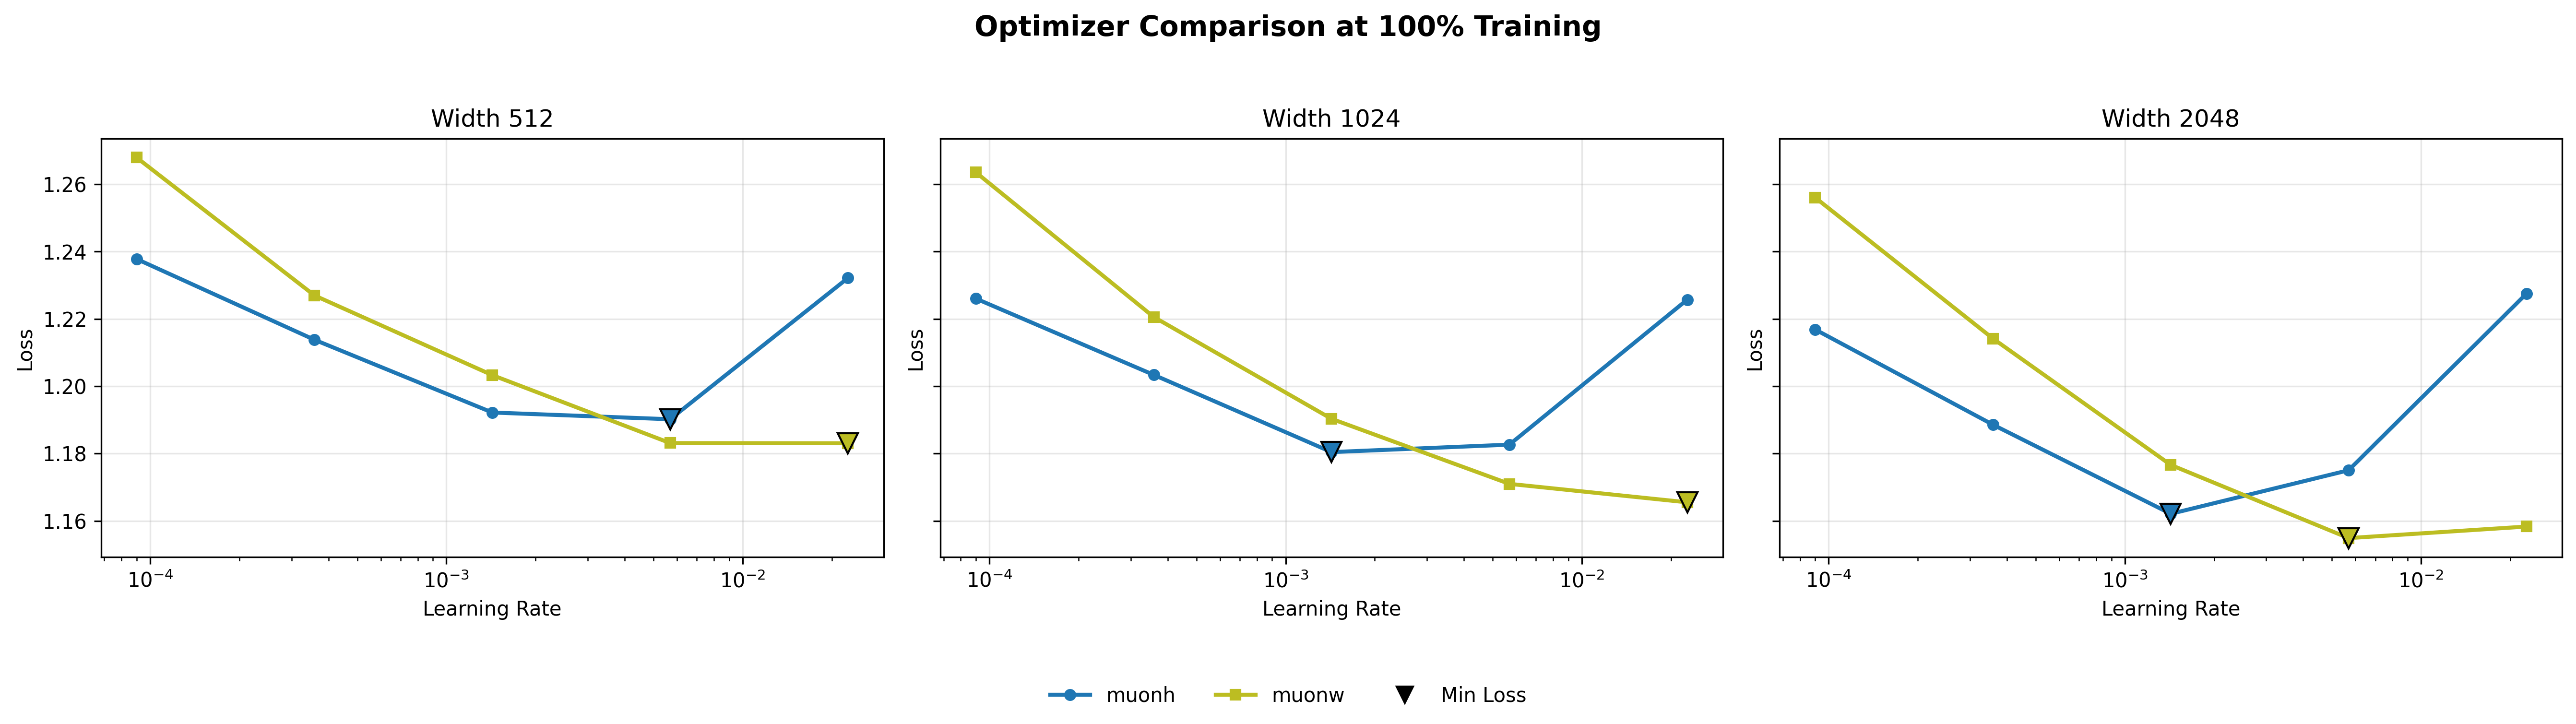
\includegraphics[width=0.85\linewidth]{images/muon_comparison.png}
  \caption{Sweep losses: MuonW vs MuonH.}
  \label{fig:sweep-losses-muon}
\end{figure}

\begin{figure}[htbp]
  \centering
  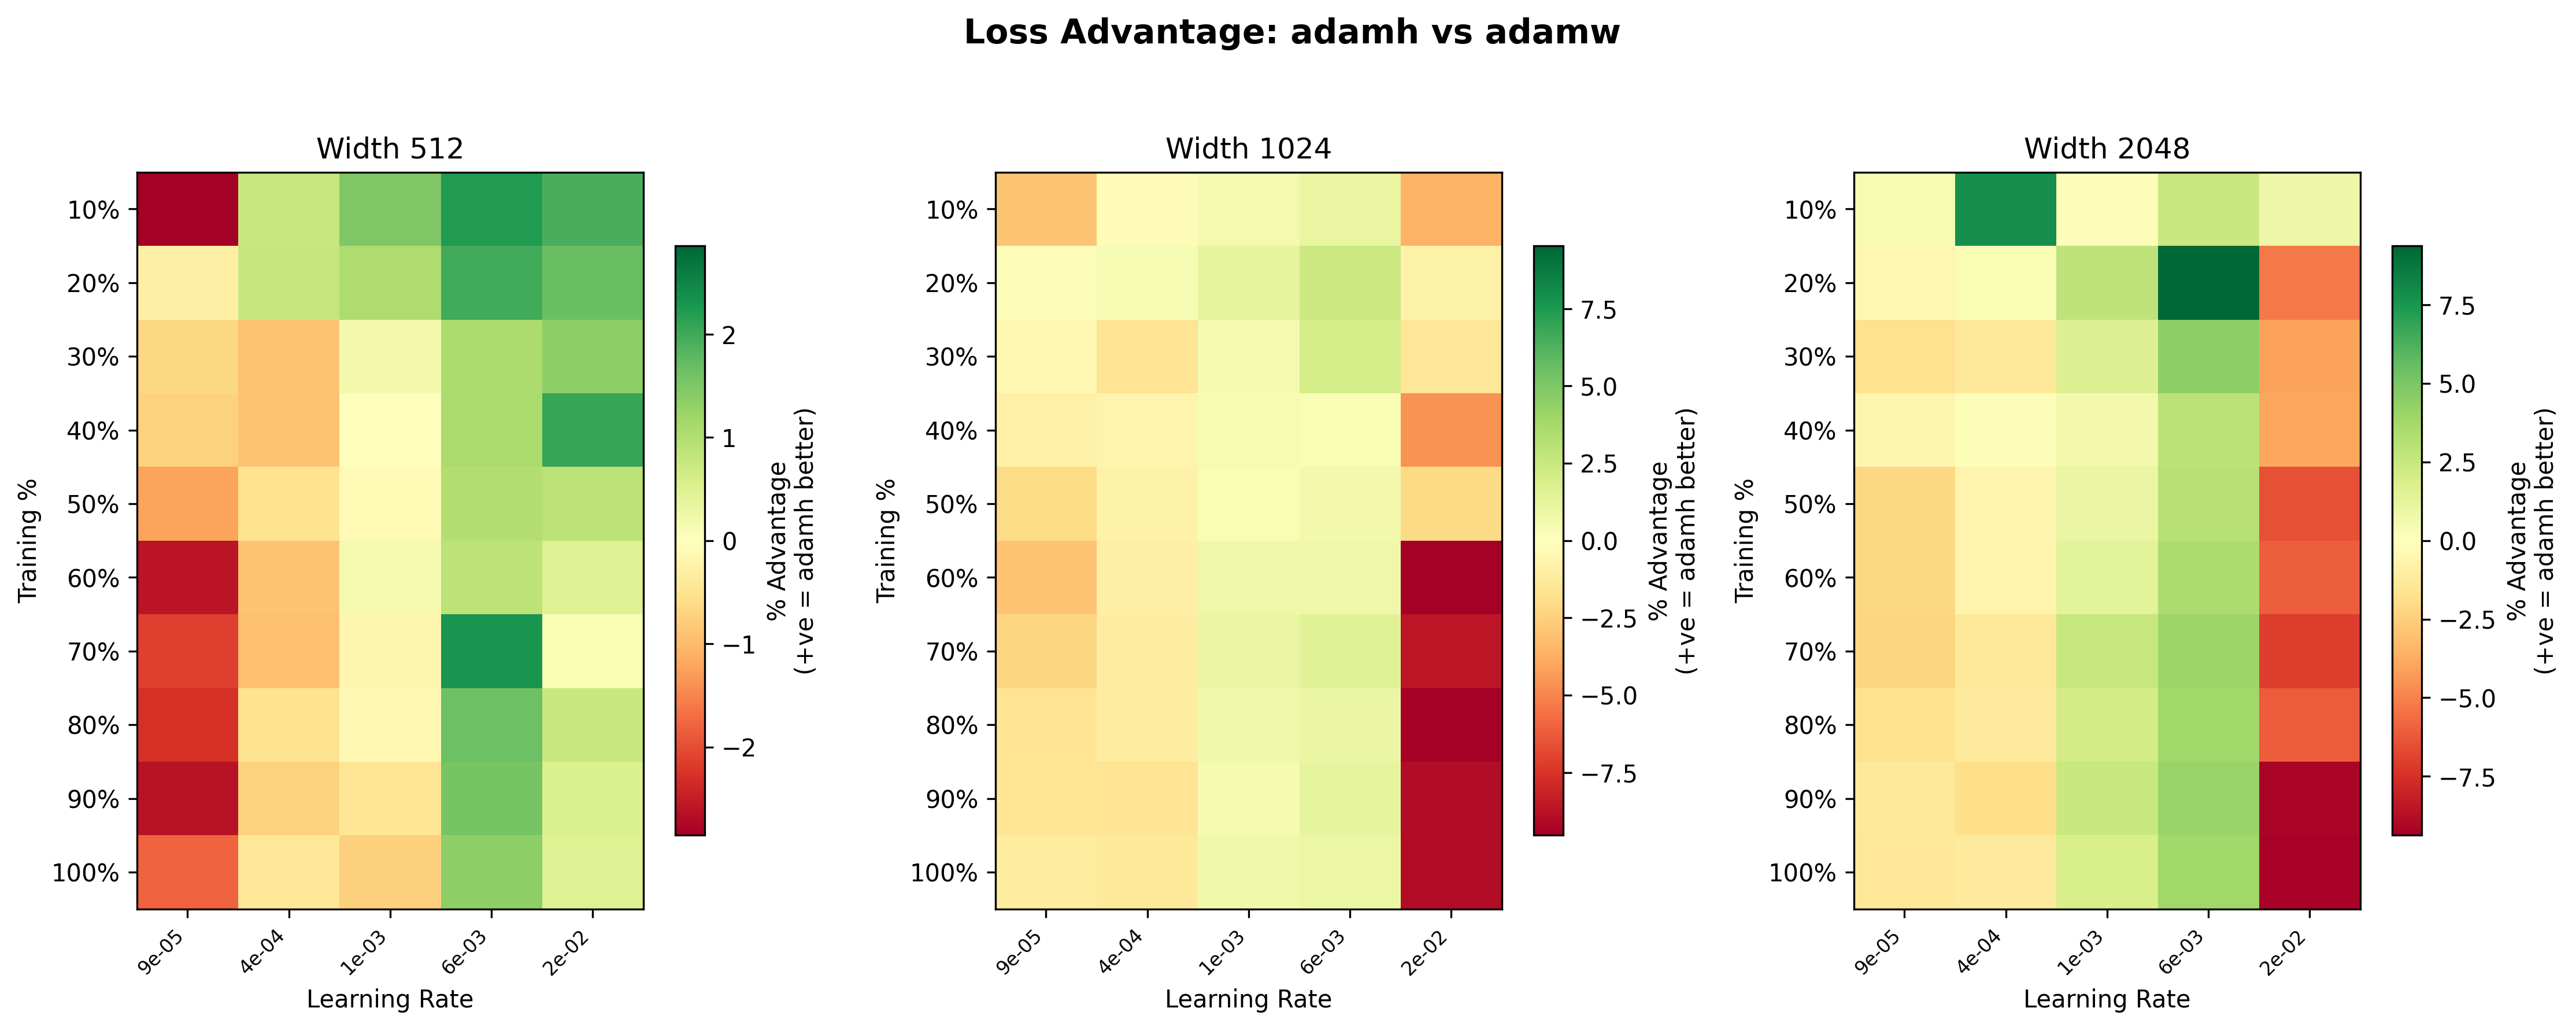
\includegraphics[width=0.85\linewidth]{images/adam_heatmap.png}
  \caption{Heatmap: AdamW vs AdamH.}
  \label{fig:heatmap-adam}
\end{figure}

\begin{figure}[htbp]
  \centering
  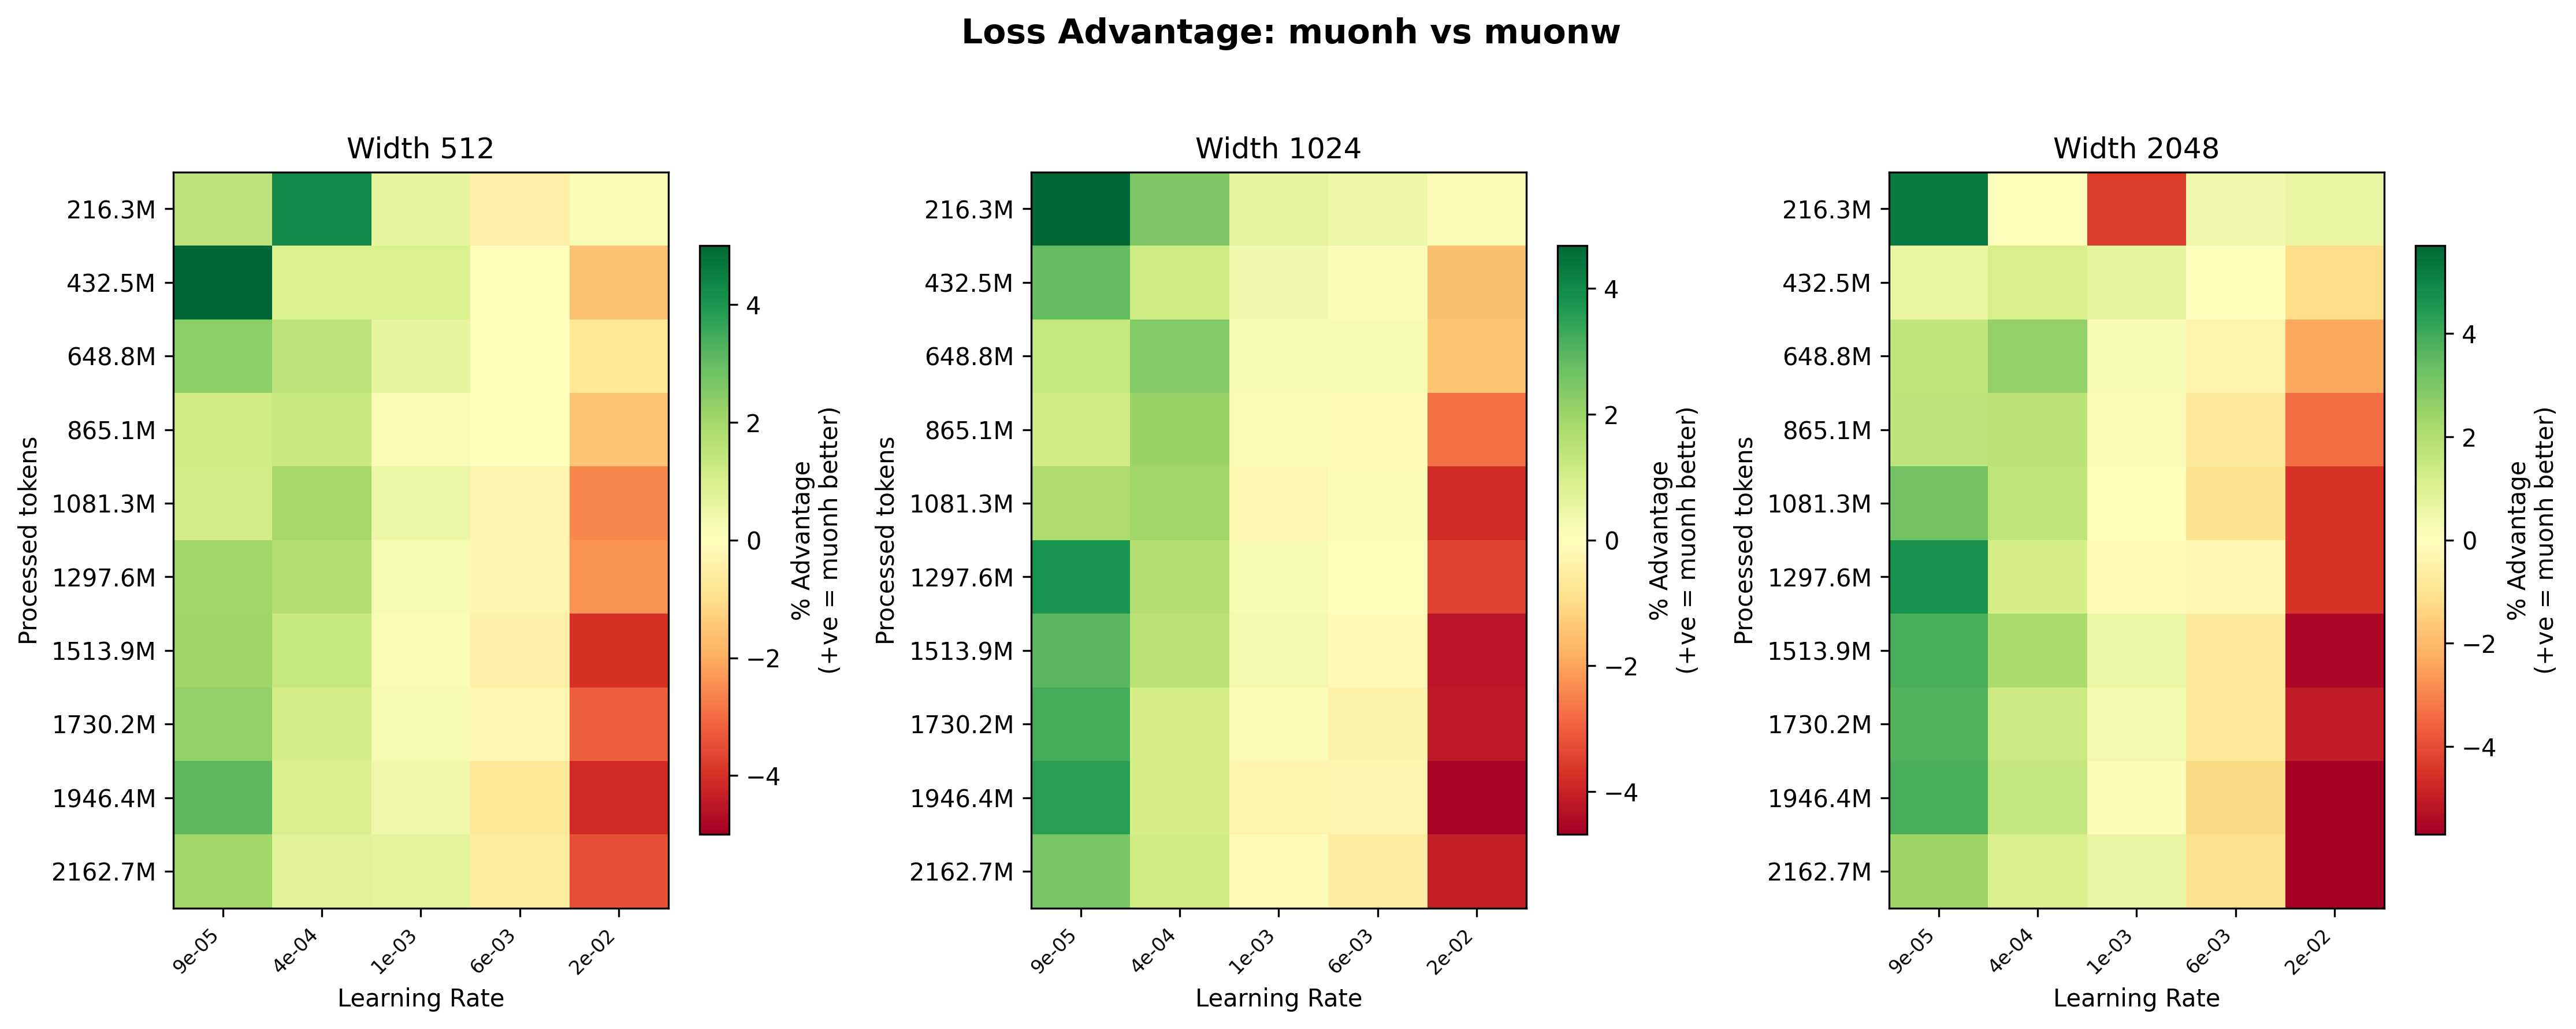
\includegraphics[width=0.85\linewidth]{images/muon_heatmap.png}
  \caption{Heatmap: MuonW vs MuonH.}
  \label{fig:heatmap-muon}
\end{figure}

\begin{figure}[htbp]
  \centering
  
\includegraphics[width=0.85\linewidth]{images/muonw_adamh_heatmap.png}
  \caption{MuonW--AdamH advantage heatmap.}
  \label{fig:cross-optimizer-heatmap}
\end{figure}

Green indicates AdamH better, and red indicates MuonW better.

\begin{figure}[htbp]
  \centering
  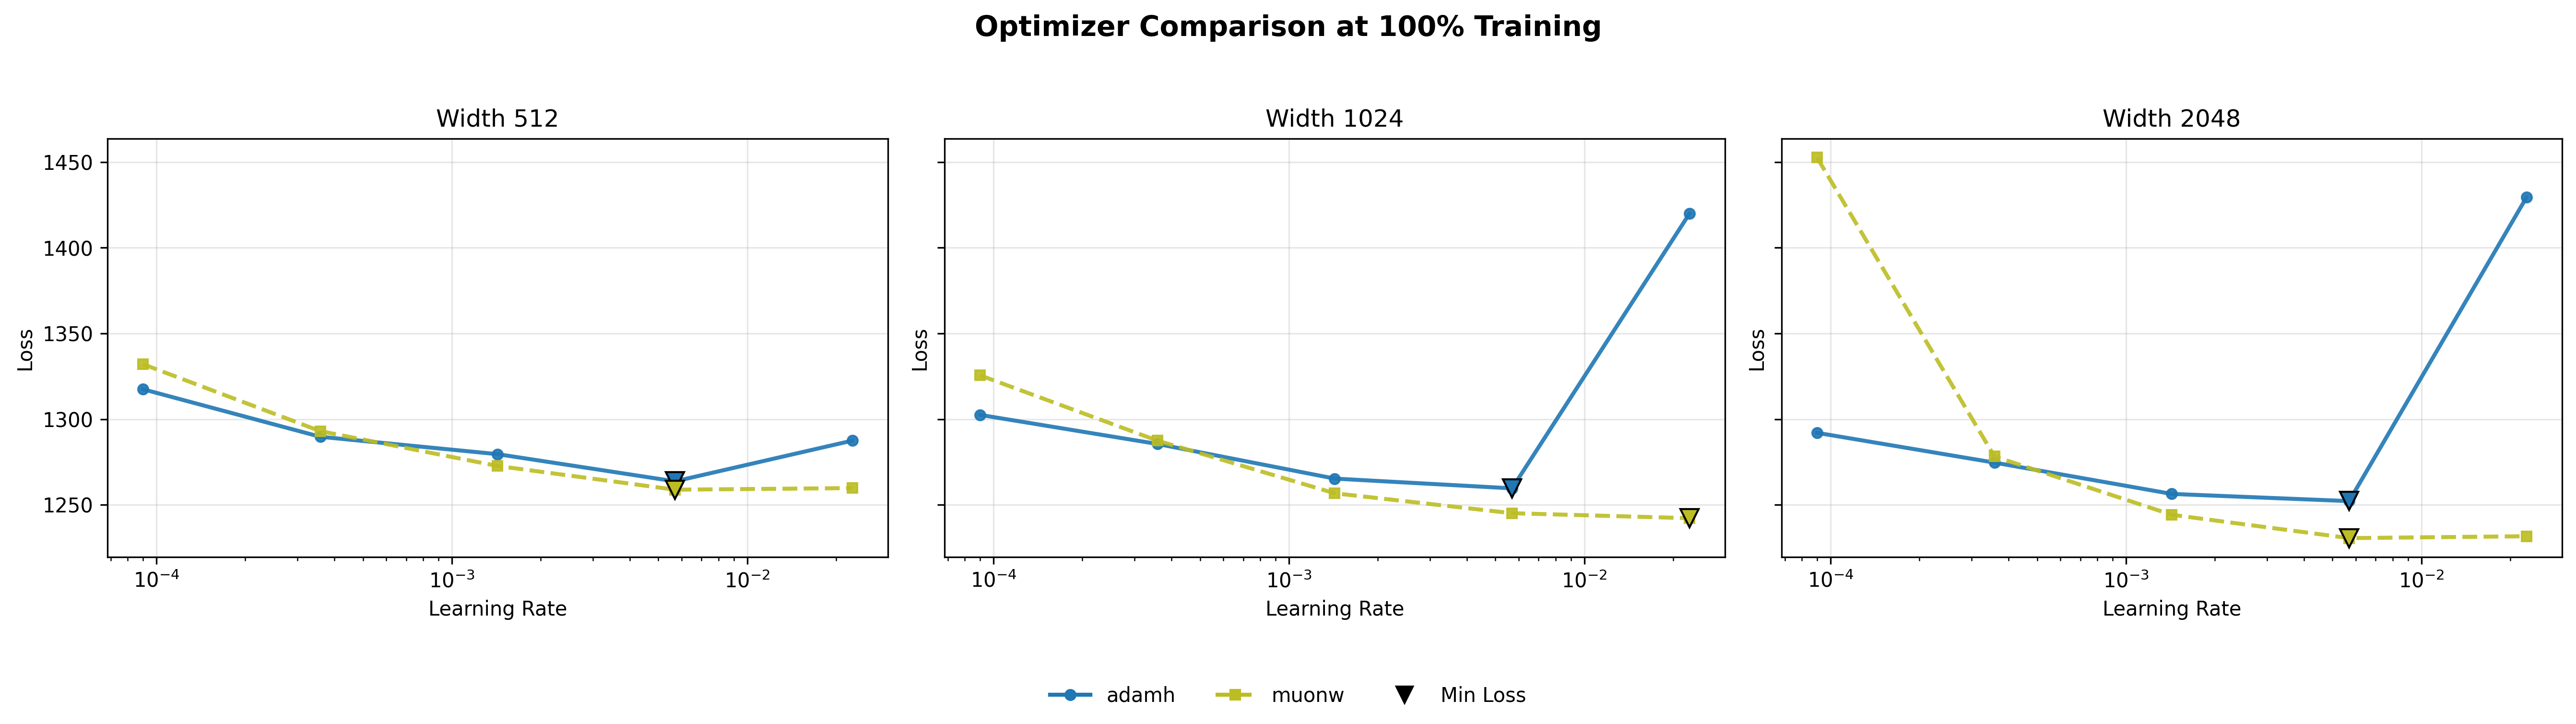
\includegraphics[width=0.85\linewidth]{images/muonw_adamh_comparison.png}
  \caption{Sweep losses for MuonW vs AdamH across widths.}
  \label{fig:cross-optimizer-sweep}
\end{figure}

\begin{figure}[htbp]
  \centering
  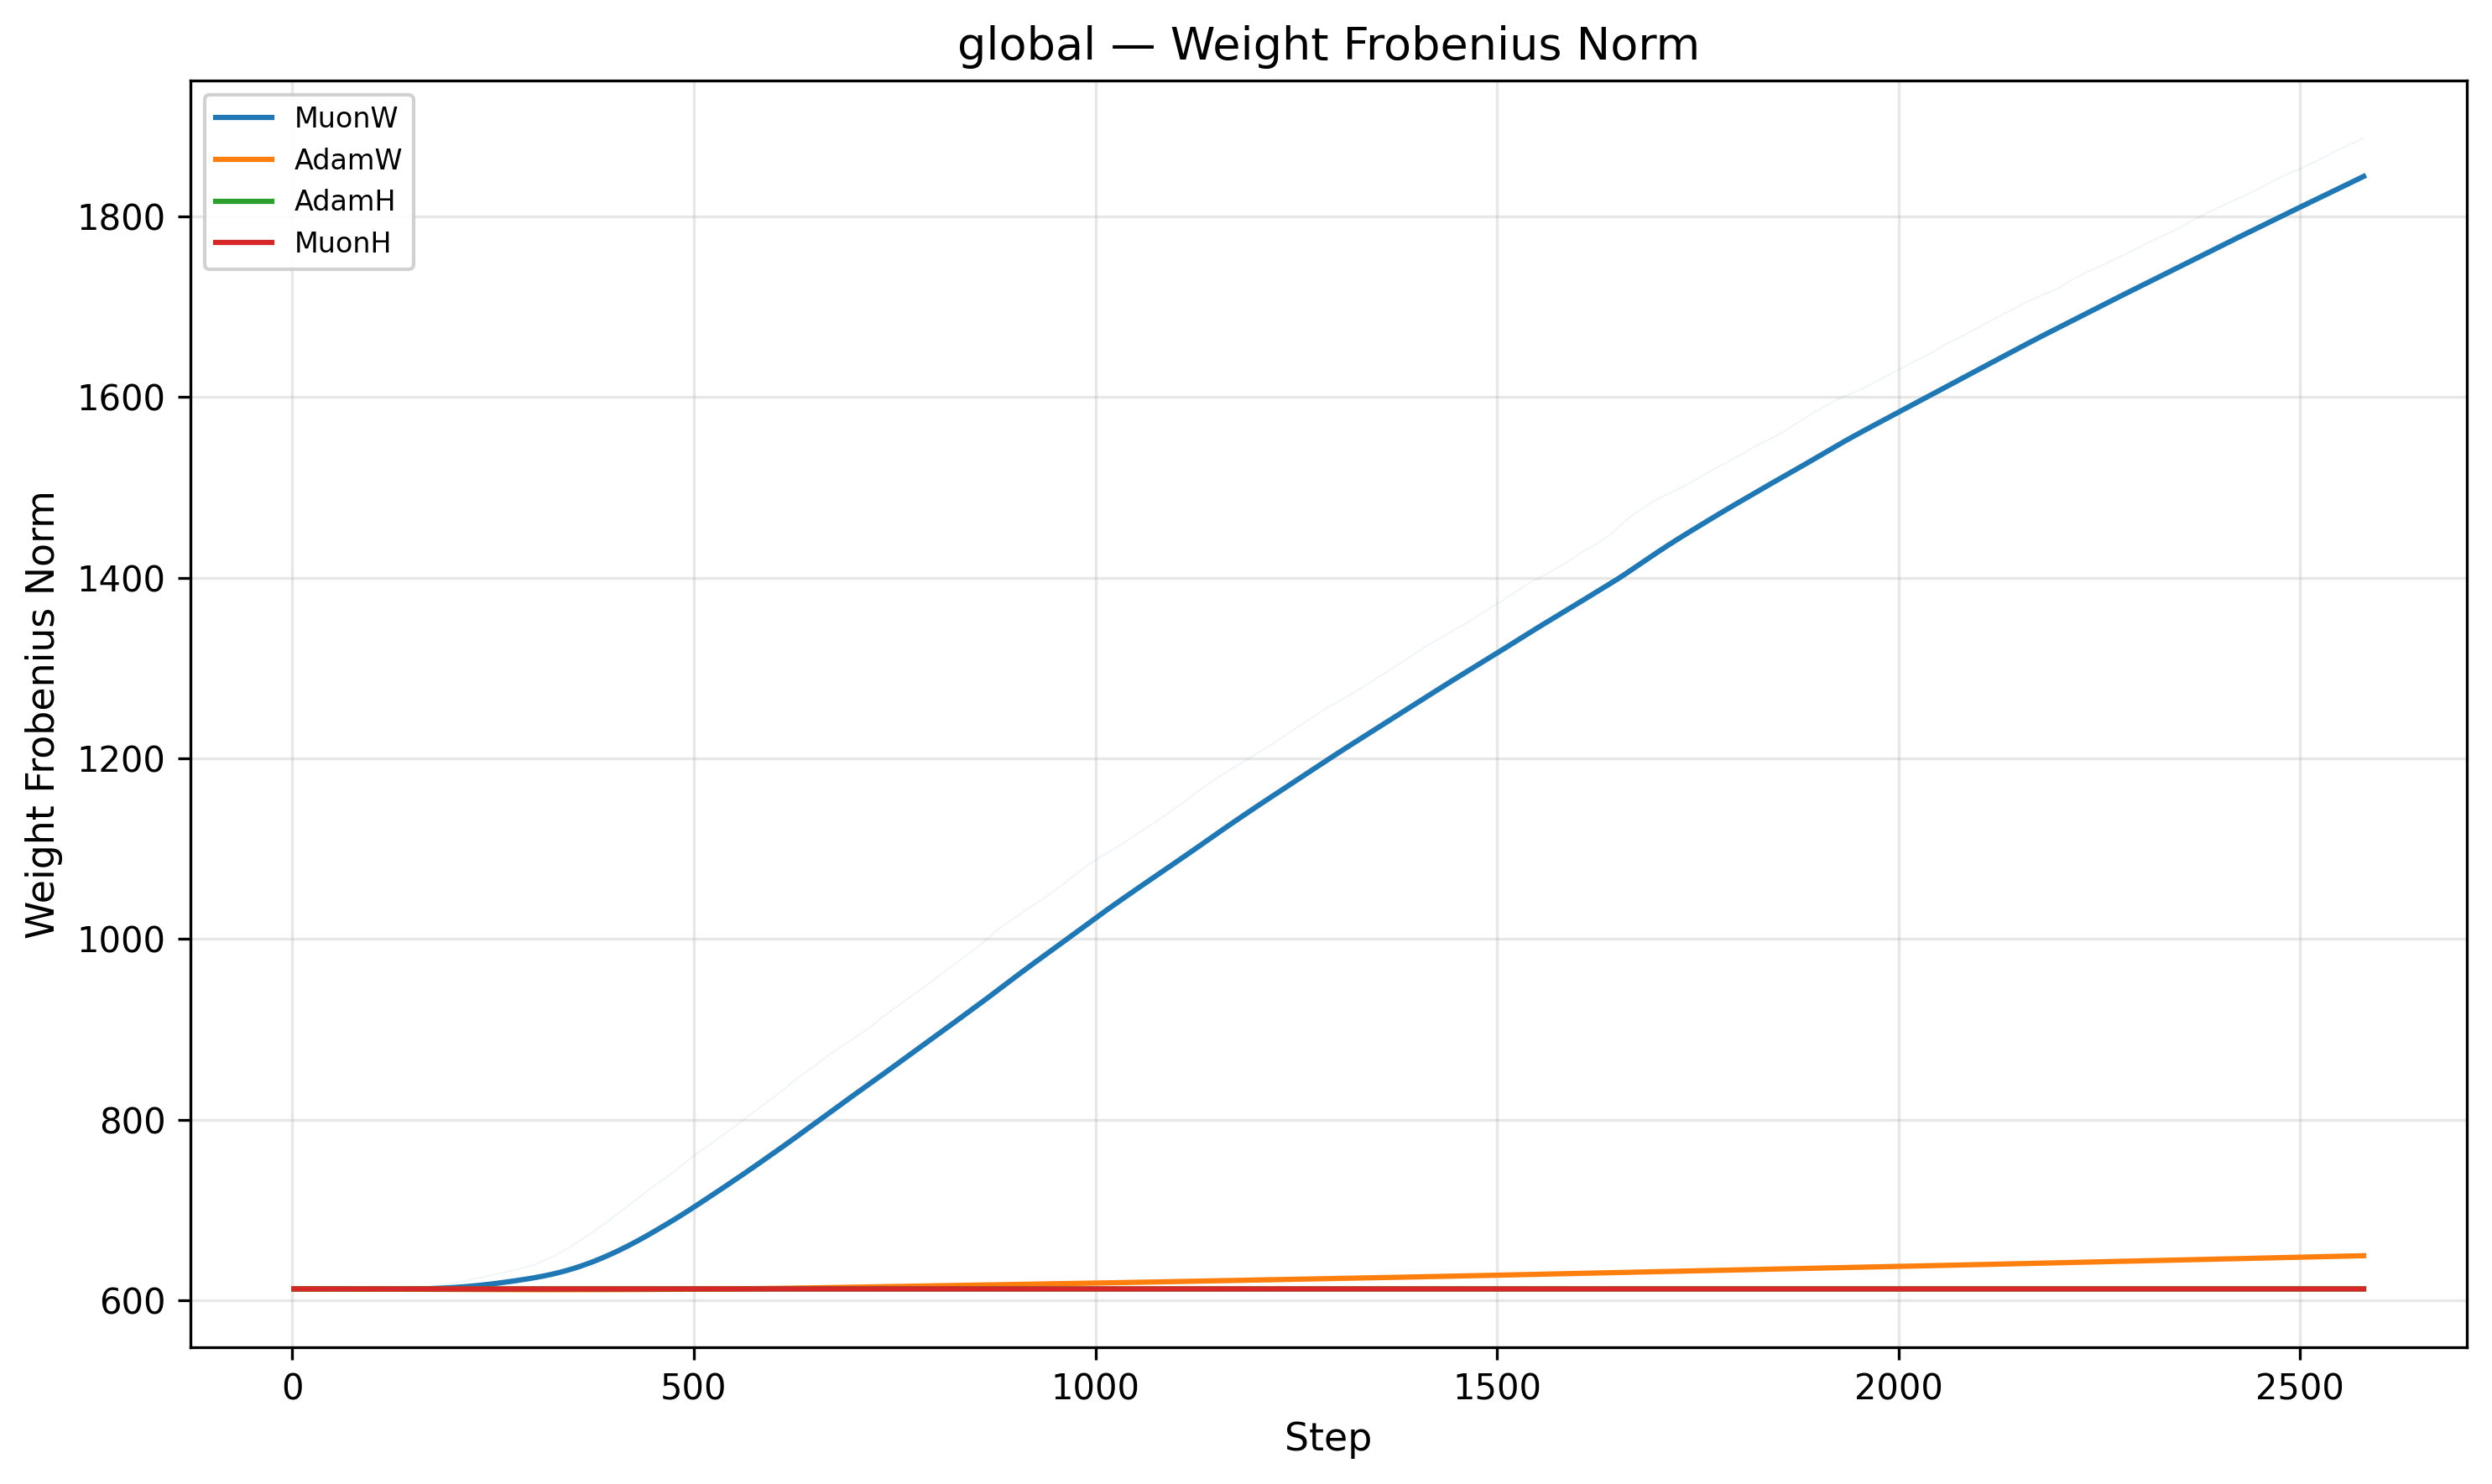
\includegraphics[width=0.85\linewidth]{images/weight_frobenius_norm.png}\\[0.5em]
  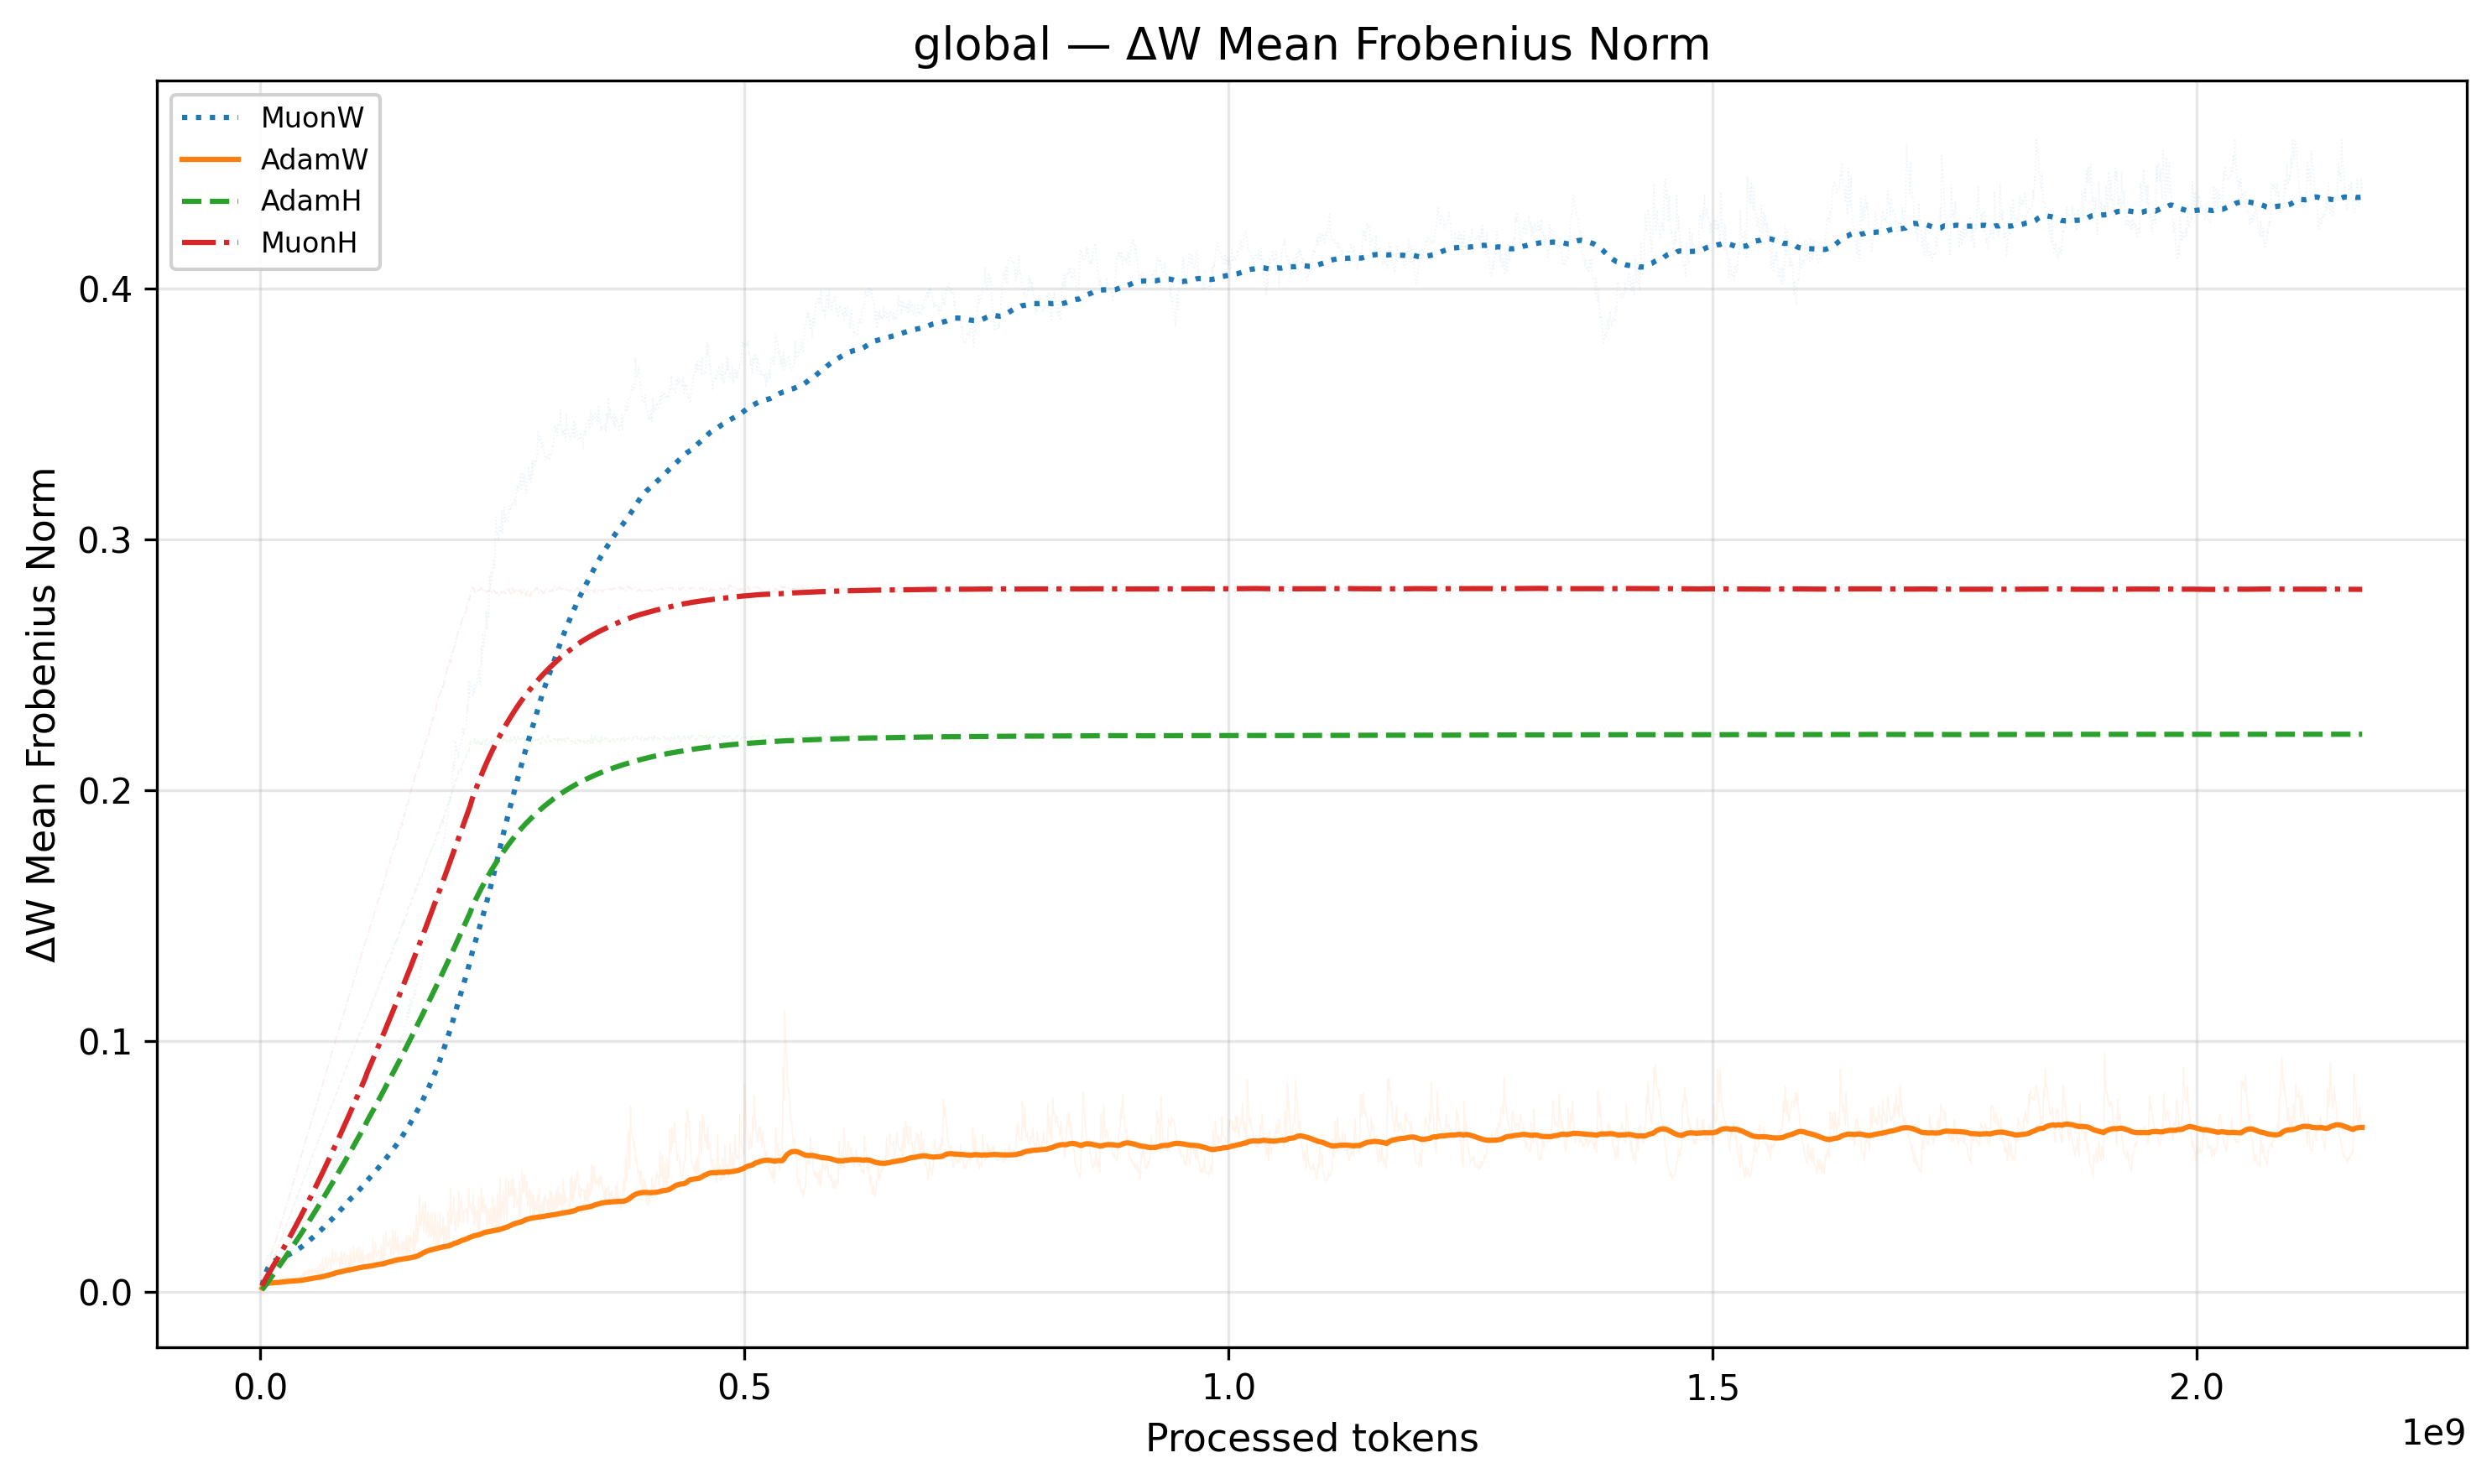
\includegraphics[width=0.85\linewidth]{images/delta_W_mean_frobenius_norm.png}
  \caption{Weight and update norms.}
  \label{fig:dynamics-norms}
\end{figure}

The top panel shows weight Frobenius norm, and the bottom panel shows update mean Frobenius norm. MuonW shows monotonically increasing weight norm with roughly constant update norm.

% ============================================================
% References
% ============================================================
\clearpage
\bibliographystyle{unsrtnat}
\bibliography{references}

\section*{NeurIPS Paper Checklist}

\begin{enumerate}

\item {\bf Claims}
    \item[] Question: Do the main claims made in the abstract and introduction accurately reflect the paper's contributions and scope?
    \item[] Answer: \answerTODO{} % Replace by \answerYes{}, \answerNo{}, or \answerNA{}.
    \item[] Justification: \justificationTODO{}
    \item[] Guidelines:
    \begin{itemize}
        \item The answer \answerNA{} means that the abstract and introduction do not include the claims made in the paper.
        \item The abstract and/or introduction should clearly state the claims made, including the contributions made in the paper and important assumptions and limitations. A \answerNo{} or \answerNA{} answer to this question will not be perceived well by the reviewers. 
        \item The claims made should match theoretical and experimental results, and reflect how much the results can be expected to generalize to other settings. 
        \item It is fine to include aspirational goals as motivation as long as it is clear that these goals are not attained by the paper. 
    \end{itemize}

\item {\bf Limitations}
    \item[] Question: Does the paper discuss the limitations of the work performed by the authors?
    \item[] Answer: \answerTODO{} % Replace by \answerYes{}, \answerNo{}, or \answerNA{}.
    \item[] Justification: \justificationTODO{}
    \item[] Guidelines:
    \begin{itemize}
        \item The answer \answerNA{} means that the paper has no limitation while the answer \answerNo{} means that the paper has limitations, but those are not discussed in the paper. 
        \item The authors are encouraged to create a separate ``Limitations'' section in their paper.
        \item The paper should point out any strong assumptions and how robust the results are to violations of these assumptions (e.g., independence assumptions, noiseless settings, model well-specification, asymptotic approximations only holding locally). The authors should reflect on how these assumptions might be violated in practice and what the implications would be.
        \item The authors should reflect on the scope of the claims made, e.g., if the approach was only tested on a few datasets or with a few runs. In general, empirical results often depend on implicit assumptions, which should be articulated.
        \item The authors should reflect on the factors that influence the performance of the approach. For example, a facial recognition algorithm may perform poorly when image resolution is low or images are taken in low lighting. Or a speech-to-text system might not be used reliably to provide closed captions for online lectures because it fails to handle technical jargon.
        \item The authors should discuss the computational efficiency of the proposed algorithms and how they scale with dataset size.
        \item If applicable, the authors should discuss possible limitations of their approach to address problems of privacy and fairness.
        \item While the authors might fear that complete honesty about limitations might be used by reviewers as grounds for rejection, a worse outcome might be that reviewers discover limitations that aren't acknowledged in the paper. The authors should use their best judgment and recognize that individual actions in favor of transparency play an important role in developing norms that preserve the integrity of the community. Reviewers will be specifically instructed to not penalize honesty concerning limitations.
    \end{itemize}

\item {\bf Theory assumptions and proofs}
    \item[] Question: For each theoretical result, does the paper provide the full set of assumptions and a complete (and correct) proof?
    \item[] Answer: \answerTODO{} % Replace by \answerYes{}, \answerNo{}, or \answerNA{}.
    \item[] Justification: \justificationTODO{}
    \item[] Guidelines:
    \begin{itemize}
        \item The answer \answerNA{} means that the paper does not include theoretical results. 
        \item All the theorems, formulas, and proofs in the paper should be numbered and cross-referenced.
        \item All assumptions should be clearly stated or referenced in the statement of any theorems.
        \item The proofs can either appear in the main paper or the supplemental material, but if they appear in the supplemental material, the authors are encouraged to provide a short proof sketch to provide intuition. 
        \item Inversely, any informal proof provided in the core of the paper should be complemented by formal proofs provided in appendix or supplemental material.
        \item Theorems and Lemmas that the proof relies upon should be properly referenced. 
    \end{itemize}

    \item {\bf Experimental result reproducibility}
    \item[] Question: Does the paper fully disclose all the information needed to reproduce the main experimental results of the paper to the extent that it affects the main claims and/or conclusions of the paper (regardless of whether the code and data are provided or not)?
    \item[] Answer: \answerTODO{} % Replace by \answerYes{}, \answerNo{}, or \answerNA{}.
    \item[] Justification: \justificationTODO{}
    \item[] Guidelines:
    \begin{itemize}
        \item The answer \answerNA{} means that the paper does not include experiments.
        \item If the paper includes experiments, a \answerNo{} answer to this question will not be perceived well by the reviewers: Making the paper reproducible is important, regardless of whether the code and data are provided or not.
        \item If the contribution is a dataset and\slash or model, the authors should describe the steps taken to make their results reproducible or verifiable. 
        \item Depending on the contribution, reproducibility can be accomplished in various ways. For example, if the contribution is a novel architecture, describing the architecture fully might suffice, or if the contribution is a specific model and empirical evaluation, it may be necessary to either make it possible for others to replicate the model with the same dataset, or provide access to the model. In general. releasing code and data is often one good way to accomplish this, but reproducibility can also be provided via detailed instructions for how to replicate the results, access to a hosted model (e.g., in the case of a large language model), releasing of a model checkpoint, or other means that are appropriate to the research performed.
        \item While NeurIPS does not require releasing code, the conference does require all submissions to provide some reasonable avenue for reproducibility, which may depend on the nature of the contribution. For example
        \begin{enumerate}
            \item If the contribution is primarily a new algorithm, the paper should make it clear how to reproduce that algorithm.
            \item If the contribution is primarily a new model architecture, the paper should describe the architecture clearly and fully.
            \item If the contribution is a new model (e.g., a large language model), then there should either be a way to access this model for reproducing the results or a way to reproduce the model (e.g., with an open-source dataset or instructions for how to construct the dataset).
            \item We recognize that reproducibility may be tricky in some cases, in which case authors are welcome to describe the particular way they provide for reproducibility. In the case of closed-source models, it may be that access to the model is limited in some way (e.g., to registered users), but it should be possible for other researchers to have some path to reproducing or verifying the results.
        \end{enumerate}
    \end{itemize}


\item {\bf Open access to data and code}
    \item[] Question: Does the paper provide open access to the data and code, with sufficient instructions to faithfully reproduce the main experimental results, as described in supplemental material?
    \item[] Answer: \answerTODO{} % Replace by \answerYes{}, \answerNo{}, or \answerNA{}.
    \item[] Justification: \justificationTODO{}
    \item[] Guidelines:
    \begin{itemize}
        \item The answer \answerNA{} means that paper does not include experiments requiring code.
        \item Please see the NeurIPS code and data submission guidelines (\url{https://neurips.cc/public/guides/CodeSubmissionPolicy}) for more details.
        \item While we encourage the release of code and data, we understand that this might not be possible, so \answerNo{} is an acceptable answer. Papers cannot be rejected simply for not including code, unless this is central to the contribution (e.g., for a new open-source benchmark).
        \item The instructions should contain the exact command and environment needed to run to reproduce the results. See the NeurIPS code and data submission guidelines (\url{https://neurips.cc/public/guides/CodeSubmissionPolicy}) for more details.
        \item The authors should provide instructions on data access and preparation, including how to access the raw data, preprocessed data, intermediate data, and generated data, etc.
        \item The authors should provide scripts to reproduce all experimental results for the new proposed method and baselines. If only a subset of experiments are reproducible, they should state which ones are omitted from the script and why.
        \item At submission time, to preserve anonymity, the authors should release anonymized versions (if applicable).
        \item Providing as much information as possible in supplemental material (appended to the paper) is recommended, but including URLs to data and code is permitted.
    \end{itemize}


\item {\bf Experimental setting/details}
    \item[] Question: Does the paper specify all the training and test details (e.g., data splits, hyperparameters, how they were chosen, type of optimizer) necessary to understand the results?
    \item[] Answer: \answerTODO{} % Replace by \answerYes{}, \answerNo{}, or \answerNA{}.
    \item[] Justification: \justificationTODO{}
    \item[] Guidelines:
    \begin{itemize}
        \item The answer \answerNA{} means that the paper does not include experiments.
        \item The experimental setting should be presented in the core of the paper to a level of detail that is necessary to appreciate the results and make sense of them.
        \item The full details can be provided either with the code, in appendix, or as supplemental material.
    \end{itemize}

\item {\bf Experiment statistical significance}
    \item[] Question: Does the paper report error bars suitably and correctly defined or other appropriate information about the statistical significance of the experiments?
    \item[] Answer: \answerTODO{} % Replace by \answerYes{}, \answerNo{}, or \answerNA{}.
    \item[] Justification: \justificationTODO{}
    \item[] Guidelines:
    \begin{itemize}
        \item The answer \answerNA{} means that the paper does not include experiments.
        \item The authors should answer \answerYes{} if the results are accompanied by error bars, confidence intervals, or statistical significance tests, at least for the experiments that support the main claims of the paper.
        \item The factors of variability that the error bars are capturing should be clearly stated (for example, train/test split, initialization, random drawing of some parameter, or overall run with given experimental conditions).
        \item The method for calculating the error bars should be explained (closed form formula, call to a library function, bootstrap, etc.)
        \item The assumptions made should be given (e.g., Normally distributed errors).
        \item It should be clear whether the error bar is the standard deviation or the standard error of the mean.
        \item It is OK to report 1-sigma error bars, but one should state it. The authors should preferably report a 2-sigma error bar than state that they have a 96\% CI, if the hypothesis of Normality of errors is not verified.
        \item For asymmetric distributions, the authors should be careful not to show in tables or figures symmetric error bars that would yield results that are out of range (e.g., negative error rates).
        \item If error bars are reported in tables or plots, the authors should explain in the text how they were calculated and reference the corresponding figures or tables in the text.
    \end{itemize}

\item {\bf Experiments compute resources}
    \item[] Question: For each experiment, does the paper provide sufficient information on the computer resources (type of compute workers, memory, time of execution) needed to reproduce the experiments?
    \item[] Answer: \answerTODO{} % Replace by \answerYes{}, \answerNo{}, or \answerNA{}.
    \item[] Justification: \justificationTODO{}
    \item[] Guidelines:
    \begin{itemize}
        \item The answer \answerNA{} means that the paper does not include experiments.
        \item The paper should indicate the type of compute workers CPU or GPU, internal cluster, or cloud provider, including relevant memory and storage.
        \item The paper should provide the amount of compute required for each of the individual experimental runs as well as estimate the total compute. 
        \item The paper should disclose whether the full research project required more compute than the experiments reported in the paper (e.g., preliminary or failed experiments that didn't make it into the paper). 
    \end{itemize}
    
\item {\bf Code of ethics}
    \item[] Question: Does the research conducted in the paper conform, in every respect, with the NeurIPS Code of Ethics \url{https://neurips.cc/public/EthicsGuidelines}?
    \item[] Answer: \answerTODO{} % Replace by \answerYes{}, \answerNo{}, or \answerNA{}.
    \item[] Justification: \justificationTODO{}
    \item[] Guidelines:
    \begin{itemize}
        \item The answer \answerNA{} means that the authors have not reviewed the NeurIPS Code of Ethics.
        \item If the authors answer \answerNo, they should explain the special circumstances that require a deviation from the Code of Ethics.
        \item The authors should make sure to preserve anonymity (e.g., if there is a special consideration due to laws or regulations in their jurisdiction).
    \end{itemize}


\item {\bf Broader impacts}
    \item[] Question: Does the paper discuss both potential positive societal impacts and negative societal impacts of the work performed?
    \item[] Answer: \answerTODO{} % Replace by \answerYes{}, \answerNo{}, or \answerNA{}.
    \item[] Justification: \justificationTODO{}
    \item[] Guidelines:
    \begin{itemize}
        \item The answer \answerNA{} means that there is no societal impact of the work performed.
        \item If the authors answer \answerNA{} or \answerNo, they should explain why their work has no societal impact or why the paper does not address societal impact.
        \item Examples of negative societal impacts include potential malicious or unintended uses (e.g., disinformation, generating fake profiles, surveillance), fairness considerations (e.g., deployment of technologies that could make decisions that unfairly impact specific groups), privacy considerations, and security considerations.
        \item The conference expects that many papers will be foundational research and not tied to particular applications, let alone deployments. However, if there is a direct path to any negative applications, the authors should point it out. For example, it is legitimate to point out that an improvement in the quality of generative models could be used to generate Deepfakes for disinformation. On the other hand, it is not needed to point out that a generic algorithm for optimizing neural networks could enable people to train models that generate Deepfakes faster.
        \item The authors should consider possible harms that could arise when the technology is being used as intended and functioning correctly, harms that could arise when the technology is being used as intended but gives incorrect results, and harms following from (intentional or unintentional) misuse of the technology.
        \item If there are negative societal impacts, the authors could also discuss possible mitigation strategies (e.g., gated release of models, providing defenses in addition to attacks, mechanisms for monitoring misuse, mechanisms to monitor how a system learns from feedback over time, improving the efficiency and accessibility of ML).
    \end{itemize}
    
\item {\bf Safeguards}
    \item[] Question: Does the paper describe safeguards that have been put in place for responsible release of data or models that have a high risk for misuse (e.g., pre-trained language models, image generators, or scraped datasets)?
    \item[] Answer: \answerTODO{} % Replace by \answerYes{}, \answerNo{}, or \answerNA{}.
    \item[] Justification: \justificationTODO{}
    \item[] Guidelines:
    \begin{itemize}
        \item The answer \answerNA{} means that the paper poses no such risks.
        \item Released models that have a high risk for misuse or dual-use should be released with necessary safeguards to allow for controlled use of the model, for example by requiring that users adhere to usage guidelines or restrictions to access the model or implementing safety filters. 
        \item Datasets that have been scraped from the Internet could pose safety risks. The authors should describe how they avoided releasing unsafe images.
        \item We recognize that providing effective safeguards is challenging, and many papers do not require this, but we encourage authors to take this into account and make a best faith effort.
    \end{itemize}

\item {\bf Licenses for existing assets}
    \item[] Question: Are the creators or original owners of assets (e.g., code, data, models), used in the paper, properly credited and are the license and terms of use explicitly mentioned and properly respected?
    \item[] Answer: \answerTODO{} % Replace by \answerYes{}, \answerNo{}, or \answerNA{}.
    \item[] Justification: \justificationTODO{}
    \item[] Guidelines:
    \begin{itemize}
        \item The answer \answerNA{} means that the paper does not use existing assets.
        \item The authors should cite the original paper that produced the code package or dataset.
        \item The authors should state which version of the asset is used and, if possible, include a URL.
        \item The name of the license (e.g., CC-BY 4.0) should be included for each asset.
        \item For scraped data from a particular source (e.g., website), the copyright and terms of service of that source should be provided.
        \item If assets are released, the license, copyright information, and terms of use in the package should be provided. For popular datasets, \url{paperswithcode.com/datasets} has curated licenses for some datasets. Their licensing guide can help determine the license of a dataset.
        \item For existing datasets that are re-packaged, both the original license and the license of the derived asset (if it has changed) should be provided.
        \item If this information is not available online, the authors are encouraged to reach out to the asset's creators.
    \end{itemize}

\item {\bf New assets}
    \item[] Question: Are new assets introduced in the paper well documented and is the documentation provided alongside the assets?
    \item[] Answer: \answerTODO{} % Replace by \answerYes{}, \answerNo{}, or \answerNA{}.
    \item[] Justification: \justificationTODO{}
    \item[] Guidelines:
    \begin{itemize}
        \item The answer \answerNA{} means that the paper does not release new assets.
        \item Researchers should communicate the details of the dataset\slash code\slash model as part of their submissions via structured templates. This includes details about training, license, limitations, etc. 
        \item The paper should discuss whether and how consent was obtained from people whose asset is used.
        \item At submission time, remember to anonymize your assets (if applicable). You can either create an anonymized URL or include an anonymized zip file.
    \end{itemize}

\item {\bf Crowdsourcing and research with human subjects}
    \item[] Question: For crowdsourcing experiments and research with human subjects, does the paper include the full text of instructions given to participants and screenshots, if applicable, as well as details about compensation (if any)? 
    \item[] Answer: \answerTODO{} % Replace by \answerYes{}, \answerNo{}, or \answerNA{}.
    \item[] Justification: \justificationTODO{}
    \item[] Guidelines:
    \begin{itemize}
        \item The answer \answerNA{} means that the paper does not involve crowdsourcing nor research with human subjects.
        \item Including this information in the supplemental material is fine, but if the main contribution of the paper involves human subjects, then as much detail as possible should be included in the main paper. 
        \item According to the NeurIPS Code of Ethics, workers involved in data collection, curation, or other labor should be paid at least the minimum wage in the country of the data collector. 
    \end{itemize}

\item {\bf Institutional review board (IRB) approvals or equivalent for research with human subjects}
    \item[] Question: Does the paper describe potential risks incurred by study participants, whether such risks were disclosed to the subjects, and whether Institutional Review Board (IRB) approvals (or an equivalent approval/review based on the requirements of your country or institution) were obtained?
    \item[] Answer: \answerTODO{} % Replace by \answerYes{}, \answerNo{}, or \answerNA{}.
    \item[] Justification: \justificationTODO{}
    \item[] Guidelines:
    \begin{itemize}
        \item The answer \answerNA{} means that the paper does not involve crowdsourcing nor research with human subjects.
        \item Depending on the country in which research is conducted, IRB approval (or equivalent) may be required for any human subjects research. If you obtained IRB approval, you should clearly state this in the paper. 
        \item We recognize that the procedures for this may vary significantly between institutions and locations, and we expect authors to adhere to the NeurIPS Code of Ethics and the guidelines for their institution. 
        \item For initial submissions, do not include any information that would break anonymity (if applicable), such as the institution conducting the review.
    \end{itemize}

\item {\bf Declaration of LLM usage}
    \item[] Question: Does the paper describe the usage of LLMs if it is an important, original, or non-standard component of the core methods in this research? Note that if the LLM is used only for writing, editing, or formatting purposes and does \emph{not} impact the core methodology, scientific rigor, or originality of the research, declaration is not required.
    %this research? 
    \item[] Answer: \answerTODO{} % Replace by \answerYes{}, \answerNo{}, or \answerNA{}.
    \item[] Justification: \justificationTODO{}
    \item[] Guidelines:
    \begin{itemize}
        \item The answer \answerNA{} means that the core method development in this research does not involve LLMs as any important, original, or non-standard components.
        \item Please refer to our LLM policy in the NeurIPS handbook for what should or should not be described.
    \end{itemize}

\end{enumerate}

\end{document}
